% --------------------------
%DIF LATEXDIFF DIFFERENCE FILE
%DIF DEL /tmp/SBWRTKmGR1/latexdiff-vc-main/main.tex   Fri Oct  9 14:04:15 2026
%DIF ADD main.tex                                     Fri Oct  9 22:52:33 2026
% Document class
% --------------------------
\documentclass[
A4paper,                % paper size A4
twoside,                % onesite or twoside printing
openright,              % doublepage cleaning ends up right side
chapterprefix=true,     % prefix for chapter marks
12pt,                   % font size
headings=normal,        % size of headings
titlepage=on            % own page for each title page
]{book}

% **************************************************
% THESIS details
% **************************************************

% **************************************************
% THESIS COVER DATA
% **************************************************
% Fill in the details of your thesis: author, title, etc. 

\def\university{Universidad Polit\'ecnica de Madrid}
\def\UNIVERSITY{UNIVERSIDAD POLIT\'ECNICA DE MADRID}
\def\universityCenter{Escuela T\'ecnica Superior de Ingenieros de Telecomunicaci\'on}
\def\PHDprogramme{Telematics Systems Engineering}

\def\author{Hugo Pascual Ad\'an}
\def\authorStudies{M.Sc. Telecommunications Engineering}
\def\thesisTitle{Anycast Routing and Data Protection: Measurement, Jurisdictional Exposure, and Geographic Control}
\def\thesisPlace{Madrid}
\def\thesisYear{2026}

\def\supervisor{Dr. Jos\'e Mar\'ia del \'Alamo Ramiro}
\def\supervisorDetails{\supervisor, Associate Professor, Universidad Polit\'ecnica de Madrid}


% **************************************************
% Settings
% **************************************************

% **************************************************
% Settings
% **************************************************
% --------------------------
% Packages
% --------------------------
\usepackage[spanish,english,es-tabla]{babel}
\usepackage[utf8]{inputenc}
\usepackage[T1]{fontenc}
\usepackage{lmodern}     % Use a modern font (that is not pixelated)
\usepackage[protrusion=true, expansion=true]{microtype}  % Use microtype to improve readability
\usepackage{amsmath,amssymb} 
\usepackage{tabularx}    % tables spanning the full text width
\usepackage{multicol}    % multi-columns in tables
\usepackage{multirow}    % multi-rows in tables
\usepackage{longtable}   % tables spanning more than one page
\usepackage{booktabs}    % nicer horizontal rules in tables
\usepackage{colortbl}    % colour for table rules
%\usepackage{ltablex}
\usepackage{setspace}
\usepackage{graphicx,graphics}   % packages to manage images
\usepackage[export]{adjustbox}
\usepackage{ragged2e} 
\usepackage{comment} 
\usepackage{blindtext}
\usepackage[acronym,nonumberlist,nomain]{glossaries}  % package for list of acronyms
\usepackage{hyperref}
\usepackage[a4paper]{geometry}
\usepackage{parskip}     % paragraph spacing (suppress indentation)
\usepackage{fancyhdr}    % personalizar encabezado
\usepackage{enumitem}
\usepackage{xcolor}
\usepackage{emptypage}   % no headers in empty pages
\usepackage[small,hang,bf]{caption}    % caption options
\usepackage{subcaption}   
\usepackage{pdfpages}
\usepackage{hyperref}
\usepackage{fvextra}
\usepackage{graphicx}
\usepackage{svg}
% TikZ
\usepackage{tikz}           % drawing custom shapes
\usetikzlibrary{
    arrows.meta,
    positioning,
    calc,
    shapes.geometric,
    fit,
    backgrounds
}

%%% BIBLIOGRAPHY
% The style used is APA. A list of available styles is available  at https://www.overleaf.com/learn/latex/Biblatex_bibliography_styles

\usepackage[
backend=biber,
style=ieee,
sorting=nyt,
doi=true,
url=false,
isbn=false,
backref=false
]{biblatex}

% The .bib files in included here
\addbibresource{references.bib}

% --------------------------
% Customize document
% --------------------------
% Define the geometry of the document
\newgeometry {top=2.5cm, bottom=2.5cm, right=2.5cm, left=2.5cm}

\setlength{\parskip}{10pt}   % Change the default value

% hiperlinks
\hypersetup{
    colorlinks=true,          % Enable colored links
    linkcolor=black,          % Color for internal links
    urlcolor=blue,
    citecolor=blue
}

% Header and footer
\fancyhf{}   % Clear the default header and footer
\renewcommand{\headrulewidth}{0.2pt}
 
\fancyhead[RO]{\nouppercase \leftmark}  % Define the header for odd and even pages
\fancyhead[LE]{\author}           % Define the header for odd and even pages
\fancyfoot[C]{\thepage}

\addto\captionsenglish{\renewcommand{\contentsname}{Table of Contents}}

% Increase indentation in lists
\newlist{mydescription}{description}{1}
\setlist[mydescription,1]{labelindent=2em, leftmargin=2em}

% Separador suave entre filas para tablas con celdas de varias líneas
% uso: \rowsep{<número de columnas>}
\newcommand{\rowsep}[1]{%
    \arrayrulecolor{black!30}%
    \cmidrule[0.3pt](lr){1-#1}%
    \arrayrulecolor{black}%
}
\newcommand{\rowgap}{\addlinespace[4pt]}       % uso: \rowgap

% ============================================================
% TikZ styles
% ============================================================

% ------------------------------------------------------------
% Nodes
% ------------------------------------------------------------

\tikzset{
    endpoint/.style={
        draw,
        rounded corners=2pt,
        minimum width=18mm,
        minimum height=10mm,
        align=center,
        fill=gray!8
    }
}

\tikzset{
    autonomoussystem/.style={
        draw,
        rounded corners=4pt,
        minimum width=18mm,
        minimum height=9mm,
        align=center,
        fill=blue!5
    }
}

\tikzset{
    router/.style={
        draw,
        circle,
        minimum size=6mm,
        inner sep=0pt,
        fill=blue!15
    }
}

\tikzset{
    ixp/.style={
        draw,
        rounded corners=2pt,
        minimum width=13mm,
        minimum height=7mm,
        align=center,
        fill=orange!15
    }
}

\tikzset{
    replica/.style={
        draw,
        rounded corners=2pt,
        minimum width=29mm,
        minimum height=9mm,
        align=center,
        fill=green!8
    }
}

\tikzset{
    anycastip/.style={
        draw,
        rounded corners=2pt,
        minimum width=25mm,
        minimum height=11mm,
        align=center,
        fill=violet!10
    }
}

% ------------------------------------------------------------
% Links
% ------------------------------------------------------------

\tikzset{
    link/.style={
        draw=black!70,
        line width=0.7pt
    }
}

\tikzset{
    transit/.style={
        draw=black!55,
        dashed,
        line width=0.7pt
    }
}

\tikzset{
    bgppath/.style={
        draw=blue!80!black,
        line width=2pt,
        ->,
        >=Latex
    }
}

\tikzset{
    shortest/.style={
        draw=green!60!black,
        dashed,
        line width=1.2pt,
        ->,
        >=Latex
    }
}

\tikzset{
    replicaLink/.style={
        draw=violet!70!black,
        dashed,
        line width=1pt,
        ->,
        >=Latex
    }
}

% ------------------------------------------------------------
% Not categorized
% ------------------------------------------------------------

\tikzset{
    tablebox/.style={
        draw=black!55,
        rounded corners=2pt,
        inner sep=4pt,
        fill=white
    }
}

\tikzset{
    header/.style={
        font=\small\bfseries,
        align=center
    }
}

\tikzset{
    hop/.style={
        font=\scriptsize,
        align=center,
        minimum width=8mm
    }
}

\tikzset{
    address/.style={
        font=\tiny,
        align=left,
        text width=34mm
    }
}

\tikzset{
    normal/.style={
        fill=blue!3
    }
}

\tikzset{
    noresponse/.style={
        fill=red!8,
        text=red!65!black
    }
}

\tikzset{
    destination/.style={
        fill=green!8,
        text=green!40!black
    }
}

% ------------------------------------------------------------
% RCA-DNS (Chapter 5)
% ------------------------------------------------------------

\tikzset{
    regionbox/.style={
        draw=black!60,
        dashed,
        rounded corners=6pt,
        inner sep=3mm,
        fill=gray!3
    }
}

\tikzset{
    regionlabel/.style={
        font=\footnotesize\bfseries,
        anchor=north west,
        inner sep=1.5mm
    }
}

\tikzset{
    policy/.style={
        draw,
        rounded corners=2pt,
        minimum width=26mm,
        minimum height=8mm,
        align=center,
        font=\footnotesize,
        fill=yellow!15
    }
}

\tikzset{
    dnszone/.style={
        draw,
        rounded corners=2pt,
        align=left,
        inner sep=2mm,
        font=\footnotesize,
        fill=orange!8
    }
}

\tikzset{
    steplabel/.style={
        circle,
        draw=black!70,
        fill=white,
        font=\scriptsize\bfseries,
        inner sep=0.8pt,
        minimum size=4.2mm
    }
}

\tikzset{
    dnsflow/.style={
        draw=orange!70!black,
        line width=1.2pt,
        ->,
        >=Latex
    }
}

\tikzset{
    lifelinehead/.style={
        draw,
        rounded corners=2pt,
        minimum width=24mm,
        minimum height=10mm,
        align=center,
        font=\footnotesize,
        fill=gray!8
    }
}

\tikzset{
    lifeline/.style={
        draw=black!45,
        dashed,
        line width=0.6pt
    }
}

\tikzset{
    msg/.style={
        draw=black!80,
        line width=0.8pt,
        ->,
        >=Latex
    }
}

\tikzset{
    reply/.style={
        draw=black!70,
        dashed,
        line width=0.8pt,
        ->,
        >=Latex
    }
}

\tikzset{
    msglabel/.style={
        font=\scriptsize,
        align=center,
        fill=white,
        inner sep=1pt
    }
}

\tikzset{
    encrypted/.style={
        draw=green!50!black,
        line width=1.4pt,
        ->,
        >=Latex
    }
}

\tikzset{
    cleartext/.style={
        draw=red!70!black,
        line width=1.4pt,
        ->,
        >=Latex
    }
}


\newcommand{\hugo}[1]{\textcolor{violet}{#1}}
\newcommand{\chema}[1]{\textcolor{green}{#1}}

% **************************************************
% Begin document?
% **************************************************
%DIF PREAMBLE EXTENSION ADDED BY LATEXDIFF
%DIF UNDERLINE PREAMBLE %DIF PREAMBLE
\RequirePackage[normalem]{ulem} %DIF PREAMBLE
\RequirePackage{color}\definecolor{RED}{rgb}{1,0,0}\definecolor{BLUE}{rgb}{0,0,1} %DIF PREAMBLE
\providecommand{\DIFaddtex}[1]{{\protect\color{blue}\uwave{#1}}} %DIF PREAMBLE
\providecommand{\DIFdeltex}[1]{{\protect\color{red}\sout{#1}}} %DIF PREAMBLE
%DIF SAFE PREAMBLE %DIF PREAMBLE
\providecommand{\DIFaddbegin}{} %DIF PREAMBLE
\providecommand{\DIFaddend}{} %DIF PREAMBLE
\providecommand{\DIFdelbegin}{} %DIF PREAMBLE
\providecommand{\DIFdelend}{} %DIF PREAMBLE
\providecommand{\DIFmodbegin}{} %DIF PREAMBLE
\providecommand{\DIFmodend}{} %DIF PREAMBLE
%DIF FLOATSAFE PREAMBLE %DIF PREAMBLE
\providecommand{\DIFaddFL}[1]{\DIFadd{#1}} %DIF PREAMBLE
\providecommand{\DIFdelFL}[1]{\DIFdel{#1}} %DIF PREAMBLE
\providecommand{\DIFaddbeginFL}{} %DIF PREAMBLE
\providecommand{\DIFaddendFL}{} %DIF PREAMBLE
\providecommand{\DIFdelbeginFL}{} %DIF PREAMBLE
\providecommand{\DIFdelendFL}{} %DIF PREAMBLE
%DIF HYPERREF PREAMBLE %DIF PREAMBLE
\providecommand{\DIFadd}[1]{\texorpdfstring{\DIFaddtex{#1}}{#1}} %DIF PREAMBLE
\providecommand{\DIFdel}[1]{\texorpdfstring{\DIFdeltex{#1}}{}} %DIF PREAMBLE
\providecommand{\DIFscaledelfig}{0.5}
%DIF HIGHLIGHTGRAPHICS PREAMBLE %DIF PREAMBLE
\RequirePackage{settobox} %DIF PREAMBLE
\RequirePackage{letltxmacro} %DIF PREAMBLE
\newsavebox{\DIFdelgraphicsbox} %DIF PREAMBLE
\newlength{\DIFdelgraphicswidth} %DIF PREAMBLE
\newlength{\DIFdelgraphicsheight} %DIF PREAMBLE
% store original definition of \includegraphics %DIF PREAMBLE
\LetLtxMacro{\DIFOincludegraphics}{\includegraphics} %DIF PREAMBLE
\providecommand{\DIFaddincludegraphics}[2][]{{\color{blue}\fbox{\DIFOincludegraphics[#1]{#2}}}} %DIF PREAMBLE
\providecommand{\DIFdelincludegraphics}[2][]{% %DIF PREAMBLE
\sbox{\DIFdelgraphicsbox}{\DIFOincludegraphics[#1]{#2}}% %DIF PREAMBLE
\settoboxwidth{\DIFdelgraphicswidth}{\DIFdelgraphicsbox} %DIF PREAMBLE
\settoboxtotalheight{\DIFdelgraphicsheight}{\DIFdelgraphicsbox} %DIF PREAMBLE
\scalebox{\DIFscaledelfig}{% %DIF PREAMBLE
\parbox[b]{\DIFdelgraphicswidth}{\usebox{\DIFdelgraphicsbox}\\[-\baselineskip] \rule{\DIFdelgraphicswidth}{0em}}\llap{\resizebox{\DIFdelgraphicswidth}{\DIFdelgraphicsheight}{% %DIF PREAMBLE
\setlength{\unitlength}{\DIFdelgraphicswidth}% %DIF PREAMBLE
\begin{picture}(1,1)% %DIF PREAMBLE
\thicklines\linethickness{2pt} %DIF PREAMBLE
{\color[rgb]{1,0,0}\put(0,0){\framebox(1,1){}}}% %DIF PREAMBLE
{\color[rgb]{1,0,0}\put(0,0){\line( 1,1){1}}}% %DIF PREAMBLE
{\color[rgb]{1,0,0}\put(0,1){\line(1,-1){1}}}% %DIF PREAMBLE
\end{picture}% %DIF PREAMBLE
}\hspace*{3pt}}} %DIF PREAMBLE
} %DIF PREAMBLE
\LetLtxMacro{\DIFOaddbegin}{\DIFaddbegin} %DIF PREAMBLE
\LetLtxMacro{\DIFOaddend}{\DIFaddend} %DIF PREAMBLE
\LetLtxMacro{\DIFOdelbegin}{\DIFdelbegin} %DIF PREAMBLE
\LetLtxMacro{\DIFOdelend}{\DIFdelend} %DIF PREAMBLE
\DeclareRobustCommand{\DIFaddbegin}{\DIFOaddbegin \let\includegraphics\DIFaddincludegraphics} %DIF PREAMBLE
\DeclareRobustCommand{\DIFaddend}{\DIFOaddend \let\includegraphics\DIFOincludegraphics} %DIF PREAMBLE
\DeclareRobustCommand{\DIFdelbegin}{\DIFOdelbegin \let\includegraphics\DIFdelincludegraphics} %DIF PREAMBLE
\DeclareRobustCommand{\DIFdelend}{\DIFOaddend \let\includegraphics\DIFOincludegraphics} %DIF PREAMBLE
\LetLtxMacro{\DIFOaddbeginFL}{\DIFaddbeginFL} %DIF PREAMBLE
\LetLtxMacro{\DIFOaddendFL}{\DIFaddendFL} %DIF PREAMBLE
\LetLtxMacro{\DIFOdelbeginFL}{\DIFdelbeginFL} %DIF PREAMBLE
\LetLtxMacro{\DIFOdelendFL}{\DIFdelendFL} %DIF PREAMBLE
\DeclareRobustCommand{\DIFaddbeginFL}{\DIFOaddbeginFL \let\includegraphics\DIFaddincludegraphics} %DIF PREAMBLE
\DeclareRobustCommand{\DIFaddendFL}{\DIFOaddendFL \let\includegraphics\DIFOincludegraphics} %DIF PREAMBLE
\DeclareRobustCommand{\DIFdelbeginFL}{\DIFOdelbeginFL \let\includegraphics\DIFdelincludegraphics} %DIF PREAMBLE
\DeclareRobustCommand{\DIFdelendFL}{\DIFOaddendFL \let\includegraphics\DIFOincludegraphics} %DIF PREAMBLE
%DIF AMSMATHULEM PREAMBLE %DIF PREAMBLE
\makeatletter %DIF PREAMBLE
\let\sout@orig\sout %DIF PREAMBLE
\renewcommand{\sout}[1]{\ifmmode\text{\sout@orig{\ensuremath{#1}}}\else\sout@orig{#1}\fi} %DIF PREAMBLE
\makeatother %DIF PREAMBLE
%DIF END PREAMBLE EXTENSION ADDED BY LATEXDIFF

\begin{document}

% --------------------------
% Cover and front matteranycast anycast 
% --------------------------
\frontmatter
\pagestyle{empty}				    % no header nor footer
% called by main.tex
\begin{center}
\begin{spacing}{1.3}
    \textbf{\large {\UNIVERSITY}}\\
    \textbf{\large {\universityCenter}}\\
    \vspace{5mm}
\end{spacing}
    
\includegraphics[width=5cm]{figures/images/EscudoETSIT.png}

\begin{spacing}{2.0}
\textbf{\LARGE {\thesisTitle}}
\end{spacing}

\vspace{15 mm}

\begin{spacing}{1.3}
\textbf{\LARGE {D\,O\,C\,T\,O\,R\,A\,L\, T\,H\,E\,S\,I\,S}}\\
\medskip
{\large {Submitted for the degree of Doctor by:}}
\end{spacing}
\end{center}


\begin{center}
\begin{spacing}{1.3}
\textbf{\Large {\author}}\\
{\large {\authorStudies}}\\
\end{spacing}
\end{center}

\vspace{\fill}

\begin{center}
   \large {\thesisPlace, \thesisYear}
\end{center}
\newpage

% called by main.tex

\begin{minipage}{0.20\textwidth}
        
\includegraphics[width = 0.9\linewidth, height = 3cm, keepaspectratio]{figures/images/EscudoETSIT.png}
\end{minipage}
\begin{minipage}{0.20\textwidth}
        
\includegraphics[width = 0.9\linewidth, height = 3cm, keepaspectratio]{figures/images/EscudoUPM.png}
\end{minipage}
\begin{minipage}{0.65\textwidth} \centering
    {\UNIVERSITY}\\
    {\universityCenter}\\
\end{minipage}

\vspace{15 mm}

\begin{center}
\begin{spacing}{1.5}
\textbf{\large {Doctoral Degree in {\PHDprogramme}}}\\
\end{spacing}
\vspace{10 mm}

\begin{spacing}{2.0}
\textbf{\LARGE {\thesisTitle}}
\end{spacing}

\vspace{15 mm}

\begin{spacing}{1.3}
\textbf{\LARGE {D\,O\,C\,T\,O\,R\,A\,L\, T\,H\,E\,S\,I\,S}}\\
\medskip
{\large {Submitted for the degree of Doctor by:}}
\end{spacing}
\end{center}


\begin{center}
\begin{spacing}{1.3}
\textbf{\Large {\author}}\\
{\large {\authorStudies}}\\
\end{spacing}
\end{center}

\vspace{5 mm}
\begin{center}
\begin{spacing}{1.3}
{Under the supervision of:}\\
    {\large {\supervisor}}\\
\end{spacing}
\end{center}

\vspace{15 mm}
\begin{center}
    \large {\thesisPlace, \thesisYear}
\end{center}

\newpage

\pagenumbering{roman}			    % roman page numbering 
\pagestyle{plain}				    % empty header, just page number in footer
% called by main.tex

\begin{spacing}{1.3}
Title: \thesisTitle \\
Author: \author \\
Doctoral Programme:	\PHDprogramme
\end{spacing}
Thesis Supervision: 
\begin{mydescription}
    \item \supervisor
\end{mydescription}

\vspace{10 mm}
External Reviewers: 

\vspace{30 mm}

Thesis Defense Committee: 


\vspace{50mm}



Thesis Defense Date: 



\vspace{\fill}
\begin{spacing}{1.0}
Funds of the work during the thesis
\end{spacing}

\cleardoublepage

% called by main.tex
%


\vspace*{\fill}
\begin{flushright} 
    \textit{Dedications}
    \vspace{15cm}
\end{flushright}
   % dedication (optional)
\cleardoublepage

% called by main.tex
%
\section*{Acknowledgement}
\label{sec::acknowledgement}
\addcontentsline{toc}{section}{Acknowledgement}

Lorem ipsum dolor sit amet, consectetur adipiscing elit, sed do eiusmod tempor incididunt ut labore et dolore magna aliqua. Ut enim ad minim veniam, quis nostrud exercitation ullamco laboris nisi ut aliquip ex ea commodo consequat. Duis aute irure dolor in reprehenderit in voluptate velit esse cillum dolore eu fugiat nulla pariatur. Excepteur sint occaecat cupidatat non proident, sunt in culpa qui officia deserunt mollit anim id est laborum.
  % acknowledgement (optional)
\newpage

% called by main.tex
%

\section*{Abstract}
\addcontentsline{toc}{section}{Abstract}
\label{sec::abstract}

Anycast routing, in which the same IP address is announced from multiple locations and the Internet routing system delivers each communication to one of them, underpins a large part of today's Internet infrastructure, including Content Delivery Networks (CDNs), cloud platforms, and the third-party services embedded in mobile applications. Although anycast improves performance and resilience, it makes the geographic destination of each communication invisible to users and largely uncontrolled by service operators, since the replica that processes a request results from distributed routing decisions in which jurisdiction plays no role. This is problematic under regulations such as the General Data Protection Regulation (GDPR), which requires transparency about where personal data are processed, particularly when they are transferred to countries outside the European Economic Area (EEA). This thesis studies how anycast affects \DIFdelbegin \DIFdel{international transfers of personal data and }\DIFdelend \DIFaddbegin \DIFadd{the geographic destination of communications carrying personal data, and therefore potential international transfers, and }\DIFaddend how geographic control can be restored without giving up the benefits of anycast.

First, the thesis presents Hunter, a methodology that infers the country in which an anycast communication terminates by combining traceroute analysis, last-hop identification, and latency-based multilateration. In a validation with ground truth covering 29 countries of the EEA and 2,739 measurements, Hunter achieved a precision of 97.67\% and an accuracy of 78.09\%, deliberately favouring conservative decisions that avoid attributing communications to the wrong jurisdiction.

Second, Hunter is applied to a large-scale analysis of 5,759 Android applications. Of the communications containing personal data, 80.74\% were directed towards anycast infrastructures, and they were generated by 960 applications. The results reveal a significant gap between \DIFdelbegin \DIFdel{declared and actual transfers}\DIFdelend \DIFaddbegin \DIFadd{the destinations declared and those observed}\DIFaddend : 98.65\% of the analysed applications did not adequately disclose in their privacy policies the destination countries observed, and 90\% of the Third-Party Libraries (TPLs) involved, all of which could reach destinations outside the EEA, did not disclose them either. A subsequent global campaign covering 183 countries and 504,690 routing tracks showed that this behaviour is not limited to EEA: 58.36\% of the tracks terminated in a country different from that of origin, and 99.49\% of the analysed anycast addresses exhibited cross-border routing.

Third, the thesis proposes Region-Constrained Anycast over DNS (RCA-DNS), an architecture that makes the region an explicit parameter of each communication. Each region is exposed through its own DNS name and anycast address, served only by infrastructure located within that region, so that the service selects the region according to its own policy while anycast continues to distribute traffic within it. The thesis analyses the levels at which this confinement can be enforced and shows that the architecture can be implemented on the main cloud and CDN platforms. A prototype deployed in 39 Google Cloud locations and evaluated with RIPE Atlas showed that, in well-provisioned regions such as the EEA, confinement \DIFdelbegin \DIFdel{entails no latencypenalty}\DIFdelend \DIFaddbegin \DIFadd{did not increase latency}\DIFaddend : compared with a global deployment, the median round-trip time decreased by 5.99\% and the 95th percentile fell from 1,252~ms to 111~ms. In regions with little infrastructure, the latency cost \DIFdelbegin \DIFdel{reflects }\DIFdelend \DIFaddbegin \DIFadd{is mainly explained by }\DIFaddend the lack of local locations\DIFdelbegin \DIFdel{rather than the mechanism itself}\DIFdelend .

Together, these contributions show that the geographic destination of anycast communications is a dynamic property that can be measured, analysed, and, through appropriate architectural mechanisms, controlled.

\newpage
\section*{Resumen}
\addcontentsline{toc}{section}{Resumen}
\label{sec::resumen}

El encaminamiento anycast, en el que una misma dirección IP se anuncia desde múltiples ubicaciones y el sistema de encaminamiento de Internet entrega cada comunicación a una de ellas, sustenta una gran parte de la infraestructura actual de Internet, incluidas las redes de distribución de contenidos (CDN), las plataformas en la nube y los servicios de terceros integrados en las aplicaciones móviles. Aunque anycast mejora el rendimiento y la resiliencia, hace que el destino geográfico de cada comunicación sea invisible para los usuarios y quede en gran medida fuera del control de los operadores de los servicios, ya que la réplica que procesa una petición resulta de decisiones de encaminamiento distribuidas en las que la jurisdicción no desempeña ningún papel. Esto resulta problemático en el marco de normativas como el Reglamento General de Protección de Datos (RGPD), que obliga a ser transparente sobre los lugares en los que se tratan los datos personales, en particular cuando se transfieren a países externos al Espacio Económico Europeo (EEE). Esta tesis estudia cómo afecta anycast \DIFdelbegin \DIFdel{a las transferencias internacionales de }\DIFdelend \DIFaddbegin \DIFadd{al destino geográfico de las comunicaciones que contienen }\DIFaddend datos personales y\DIFaddbegin \DIFadd{, por tanto, a posibles transferencias internacionales, y }\DIFaddend cómo puede recuperarse el control geográfico sin renunciar a las ventajas de anycast.

En primer lugar, la tesis presenta Hunter, una metodología que infiere el país en el que termina una comunicación anycast combinando el análisis de traceroute, la identificación del último salto y la multilateración basada en latencias. En una validación con datos de referencia que abarcó 29 países del EEE y 2.739 medidas, Hunter alcanzó una precisión del 97,67~\% y una exactitud del 78,09~\%, priorizando deliberadamente decisiones conservadoras que evitan atribuir comunicaciones a una jurisdicción errónea.

En segundo lugar, Hunter se aplica a un análisis a gran escala de 5.759 aplicaciones Android. De las comunicaciones que contenían datos personales, el 80,74~\% se dirigían a infraestructuras anycast y fueron generadas por 960 aplicaciones. Los resultados revelan una brecha significativa entre \DIFdelbegin \DIFdel{las transferencias declaradas y las reales}\DIFdelend \DIFaddbegin \DIFadd{los destinos declarados y los observados}\DIFaddend : el 98,65~\% de las aplicaciones analizadas no informaba adecuadamente en sus políticas de privacidad de los países de destino observados, y el 90~\% de las bibliotecas de terceros (TPL) implicadas, todas ellas capaces de alcanzar destinos fuera del EEE, tampoco los declaraba. Una campaña global posterior, que abarcó 183 países y 504.690 trayectorias de encaminamiento, mostró que este comportamiento no se limita al EEE: el 58,36~\% de las trayectorias terminaba en un país distinto al de origen, y el 99,49~\% de las direcciones anycast analizadas presentaba encaminamiento transfronterizo.

En tercer lugar, la tesis propone Region-Constrained Anycast over DNS (RCA-DNS), una arquitectura que convierte la región en un parámetro explícito de cada comunicación. Cada región se expone mediante su propio nombre DNS y su propia dirección anycast, servida únicamente por infraestructura situada dentro de esa región, de modo que el servicio selecciona la región según su propia política mientras anycast sigue distribuyendo el tráfico dentro de ella. La tesis analiza los niveles en los que puede aplicarse este confinamiento y muestra que la arquitectura puede implementarse en las principales plataformas en la nube y CDN. Un prototipo desplegado en 39 ubicaciones de Google Cloud y evaluado con RIPE Atlas mostró que, en regiones bien dotadas como el EEE, el confinamiento no \DIFdelbegin \DIFdel{conlleva ninguna penalización de }\DIFdelend \DIFaddbegin \DIFadd{aumentó la }\DIFaddend latencia: en comparación con un despliegue global, la mediana del tiempo de ida y vuelta disminuyó un 5,99~\% y el percentil 95 bajó de 1.252~ms a 111~ms. En regiones con poca infraestructura, el coste en latencia \DIFdelbegin \DIFdel{refleja }\DIFdelend \DIFaddbegin \DIFadd{se explica principalmente por }\DIFaddend la falta de ubicaciones locales\DIFdelbegin \DIFdel{y no el propio mecanismo}\DIFdelend .

En conjunto, estas contribuciones muestran que el destino geográfico de las comunicaciones anycast es una propiedad dinámica que puede medirse, analizarse y, mediante mecanismos arquitectónicos adecuados, controlarse.
		% abstract (in English and Spanish)
\newpage

\selectlanguage{english}

\setcounter{tocdepth}{3}		% define depth of toc
\tableofcontents				% display table of contents


\addcontentsline{toc}{section}{List of Figures}
\listoffigures


%\addcontentsline{toc}{section}{List of Tables}
%\listoftables
\newpage

% called by main.tex
%
\section*{Abbreviations and acronyms}
\addcontentsline{toc}{section}{Abbreviations and acronyms}
\label{sec::acronyns}

\vspace{10 mm}
%Institutions
\begin{description}[align=right,labelwidth=2cm] 

\item [AS] Autonomous System
\item [BGP] Border Gateway Protocol
\item [BYOIP] Bring Your Own IP
\item [CDN] Content Delivery Network
\item [DDoS] Distributed Denial-of-Service
\item [DNS] Domain Name System
\item [DSR] Design Science Research 
\item [ECS] EDNS Client Subnet extension
\item [EEA] European Economic Area
\item [GDPR] General Data Protection Regulation
\item [GFEs] Google Front Ends
\item [ISP] Internet Service Provider
\item [NEG] Network Endpoint Group
\item [PoP] Point of Presence
\item [RCA-DNS] Region-Constrained Anycast over DNS
\item [RIPE NCC] RIPE Network Coordination Centre
\item [RIR] Regional Internet Registry
\item [RFC] Request For Comments
\item [RTT] Round Trip Time
\item [SDK] Software Development Kit
\item [SNI] Server Name Indication
\item [TPLs] Third Party Libraries

\end{description}

\cleardoublepage

% --------------------------
% Main matter
% --------------------------
\mainmatter
\pagenumbering{arabic}			% arabic page numbering
\setcounter{page}{1}			% set page counter
\pagestyle{fancy} 	            % fancy header and footer
\parskip=7pt                    % space after each paragraph
\parindent=0pt                  % suppress indentation of paragraphs


% Chapters
 \newpage \chapter{Introduction}
\label{ch:introduction}

% ============================================================
\section{Context and Motivation}
\label{sc:introduction_context_motivation}
% ============================================================

The rapid evolution of digital services has led to an increasingly distributed Internet architecture. To ensure high availability, low latency, scalability, and resilience against large-scale DDoS attacks, modern Internet services rely heavily on anycast routing \cite{Abley2006OperationServices,McPherson2014ArchitecturalAnycast}. Anycast allows multiple geographically dispersed servers to share a single IP address, directing user traffic to the nearest instance according to the Internet routing topology. This paradigm has become fundamental for critical Internet services such as Content Delivery Networks (CDNs), Domain Name System (DNS) infrastructures, cloud providers, anti-DDoS platforms, and edge computing services.

Despite its operational advantages, anycast introduces a critical side effect: the logical destination of a communication no longer deterministically maps to a predictable physical location. The actual geographic endpoint reached by a user depends on highly dynamic routing decisions influenced by Border Gateway Protocol (BGP) policies, network congestion, peering agreements, failures, or traffic engineering strategies \cite{Calder2015AnalyzingCDN, Zhou2023RegionalPotentials}. Consequently, users, organisations, and even service providers may lose effective control and visibility over the countries through which personal data transits or where it is ultimately processed.

This issue becomes particularly relevant in the current regulatory landscape, where privacy, data protection, and data sovereignty have become major concerns for governments and regulatory bodies around the world. Regulations such as the General Data Protection Regulation (GDPR) in the European Economic Area (EEA) \cite{REGULATIONSRelevance}, China's Personal Information Protection Law \cite{TheTranslation}, the Australian Privacy Principles \cite{ReadOAIC}, the United Kingdom GDPR and the Data Protection Act \cite{RegulationRelevance,Data2018}, or the Protecting Americans' Data from Foreign Adversaries Act in the United States \cite{Rep.Pallone2024Text2024} establish requirements regarding the collection, processing, storage, and international transfer of personal data.

Although these regulations differ in scope and implementation, they share a common principle: organisations must maintain a certain level of control and transparency over how and where personal data is processed and transferred. However, the inherent routing dynamics of anycast challenge this assumption. A service logically deployed within a specific geographic region may silently redirect user communications to infrastructure located in foreign jurisdictions without the explicit knowledge of users, developers, or even the organisations operating the service itself.

This conflict between Internet-scale routing optimisation and legal requirements for geographic control creates a new category of privacy and compliance risks. Importantly, such risks are often invisible to end users and difficult to detect using conventional network analysis techniques. Existing privacy policies and transparency disclosures typically describe data processing from an organisational or contractual perspective, while the actual physical routing of communications remains opaque and largely uncontrolled.

Although this problem potentially affects a broad range of Internet services, this thesis focuses specifically on the Android ecosystem. Mobile applications represent one of the most pervasive sources of personal data collection in modern digital environments. Furthermore, Android applications heavily depend on Third-Party Libraries (TPLs) for functionalities such as analytics, advertising delivery, crash reporting, authentication, content distribution, and performance optimisation. These TPLs frequently have their own treatment of personal data and communicate with globally distributed infrastructures that rely on anycast-based routing mechanisms.

As a consequence, application developers may unintentionally delegate sensitive communications to third-party infrastructures whose geographic behaviour is unknown or non-deterministic. This creates a complex supply-chain privacy problem in which neither users nor developers can reliably determine where data is being transferred. In many cases, the inclusion of a single third-party dependency may silently \DIFdelbegin \DIFdel{trigger international data transfers }\DIFdelend \DIFaddbegin \DIFadd{cause personal data to reach jurisdictions }\DIFaddend that are not \DIFdelbegin \DIFdel{properly }\DIFdelend disclosed in privacy policies or that \DIFdelbegin \DIFdel{violate }\DIFdelend \DIFaddbegin \DIFadd{conflict with }\DIFaddend regional data protection \DIFdelbegin \DIFdel{constraints}\DIFdelend \DIFaddbegin \DIFadd{requirements}\DIFaddend .

In this context, understanding the relationship between anycast infrastructures, third-party ecosystems, and data protection regulations becomes essential. This thesis addresses this challenge from three complementary perspectives. First, it develops methodologies capable of accurately tracing the geographic destinations of anycast communications. Second, it evaluates the real-world privacy implications of anycast within mobile ecosystems and third-party dependencies. Finally, it proposes new architectural frameworks aimed at restoring deterministic geographic control over anycast communications while preserving the scalability and resilience benefits that motivated anycast adoption in the first place.

% ============================================================
\section{Relevance}
\label{sc:introduction_relevance}
% ============================================================

The research presented in this thesis addresses problems whose importance extends beyond the specific study of anycast routing. The increasing reliance on Cloud Computing, CDNs, edge infrastructures, and globally distributed services has transformed anycast into a fundamental building block of the modern Internet. As more applications and services depend on geographically distributed infrastructures, understanding the actual destinations reached by communications becomes increasingly relevant not only from the perspective of performance and resilience, but also in terms of privacy, data protection, international data transfers, and data sovereignty.

These concerns are reflected in several regulatory initiatives and public policies. The GDPR only permits transfers of personal data to third countries under the conditions established in Chapter~V (Articles~44--50), such as an adequacy decision of the European Commission or appropriate safeguards like standard contractual clauses \cite{REGULATIONSRelevance}. It also requires controllers to inform data subjects of their intention to transfer personal data to a third country, whether the data are collected from them (Article~13(1)(f)) or obtained from other sources (Article~14(1)(f)), and to record such transfers, including the identification of the destination country, in their records of processing activities (Article~30(1)(e)). Beyond personal data, the European Strategy for Data seeks to create common European data spaces in which European rules and values apply to the data generated and processed in the Union \cite{COMMUNICATIONData}. Building on this strategy, the Data Governance Act and the Data Act require, respectively, data intermediation services providers and providers of data processing services, among others, to take technical, organisational, and legal measures to prevent unlawful third-country governmental access to, or transfer of, non-personal data held in the Union (Article~31 and Article~32, respectively) \cite{2022DataActb, 2022DataAct}. These frameworks are analysed in more detail in Section~\ref{sc:background_privacy}. Although none of them prescribes specific networking mechanisms, all of them require organisations to know, disclose, or document where data are processed. The dynamic nature of anycast routing challenges this requirement and motivates the need for mechanisms capable of providing visibility and control over the geographic destinations reached by communications.

These concerns are reflected in several regulatory initiatives and public policies. The GDPR only permits transfers of personal data to third countries under the conditions established in Chapter~V (Articles~44--50), such as an adequacy decision of the European Commission or appropriate safeguards like standard contractual clauses \cite{REGULATIONSRelevance}. It also requires controllers to inform data subjects of their intention to transfer personal data to a third country, whether the data are collected from them (Article~13(1)(f)) or obtained from other sources (Article~14(1)(f)), and to record such transfers, including the identification of the destination country, in their records of processing activities (Article~30(1)(e)). Beyond personal data, the European Strategy for Data seeks to create common European data spaces in which European rules and values apply to the data generated and processed in the Union \cite{COMMUNICATIONData}. Building on this strategy, the Data Governance Act and the Data Act require, respectively, data intermediation services providers and providers of data processing services, among others, to take technical, organisational, and legal measures to prevent unlawful third-country governmental access to, or transfer of, non-personal data held in the Union (Article~31 and Article~32, respectively) \cite{2022DataActb, 2022DataAct}. These frameworks are analysed in more detail in Section~\ref{sc:background_privacy}. Although none of them prescribes specific networking mechanisms, all of them require organisations to know, disclose, or document where data are processed. The dynamic nature of anycast routing challenges this requirement and motivates the need for mechanisms capable of providing visibility and control over the geographic destinations reached by communications.

The objectives pursued in this thesis are also aligned with the research priorities of European and national strategic agendas. The Horizon Europe Strategic Plan 2025--2027 establishes open strategic autonomy and Europe's leading role in critical technologies as overarching principles that apply across all its key strategic orientations \cite{StrategicCommission}. These priorities have been translated into specific calls that explicitly address the location of data processing in distributed infrastructures. For instance, the topic \textit{Cognitive Cloud: AI-enabled computing continuum from Cloud to Edge} (HORIZON-CL4-2022-DATA-01-02), under which the ACES project was funded, called for cloud management layers capable of adapting to the available resources in order to ``optimize where data are being processed'' across the cloud-edge continuum, while ensuring security and data privacy \cite{CognitiveCommission}.

At the national level, the Spanish Strategy for Science, Technology and Innovation 2021--2027 aligns its strategic lines with the Horizon Europe clusters, including cybersecurity within the line on security for society, and next-generation Internet and communication networks within the line on the digital world, industry, space, and defence \cite{Estrategia2021-2027}. The National Cybersecurity Strategy also links the strengthening of research and industrial capabilities in cybersecurity with digital autonomy \cite{BOE-A-2019-6347Nacional.}. These priorities are reflected in the national funding that has supported this research: the AutoGDPR project was funded under the call for Strategic Projects Oriented towards the Ecological and Digital Transition, and the EDACCIT project under the sectoral data spaces programme of the Spanish Ministry for Digital Transformation and Public Administration, which is part of the Recovery, Transformation and Resilience Plan and is aligned with the European Strategy for Data \cite{PortalSectoriales}.In this context, the results presented in this thesis suggest that geographic control should be considered a first-class design property of distributed systems, rather than a secondary consequence of routing behaviour. As the cloud-edge continuum, data spaces, and globally distributed services continue to evolve, understanding and controlling the geographic behaviour of Internet infrastructures emerges as a promising research area at the intersection of networking, cybersecurity, cloud computing, and data protection.

From this perspective, the contributions of this thesis extend beyond the study of a particular routing mechanism. By analysing how anycast routing influences the jurisdictions reached by communications and by proposing mechanisms capable of introducing geographic constraints into service deployments, this work contributes to the broader objective of enabling distributed Internet infrastructures that simultaneously satisfy performance, resilience, transparency, and geographic control requirements. As data sovereignty and international data governance become increasingly relevant topics, understanding and controlling the geographic behaviour of Internet infrastructures is likely to become an important research challenge for both academia and industry.

% ============================================================
\section{Research Questions}
\label{sc:introduction_rqs}
% ============================================================

To address the aforementioned problem, this thesis seeks to answer the following research questions:

\begin{itemize}

    \item \textbf{RQ1 (Detection):} How can we accurately and automatically trace the geographic destination of anycast-based communications in order to identify potential cross-border personal data transfers?

    \item \textbf{RQ2 (Compliance):} To what extent do the actual geographic destinations of anycast communications align with the transparency and disclosure requirements established by current data protection legislation?

    \item \textbf{RQ3 (Ecosystem Risk):} Which software components and external dependencies contribute to the risk of unintended or non-compliant international data transfers through anycast infrastructures?

    \item \textbf{RQ4 (Mitigation):} What architectural frameworks or mechanisms can provide deterministic geographic control over anycast communications without significantly compromising scalability, performance, and resilience?

\end{itemize}

% ============================================================
\section{Thesis Objectives}
\label{sc:introduction_objectives}
% ============================================================

\subsection{Main Objective}
\label{sc:introduction_objectives_main}

The main objective of this thesis is to characterise, quantify, and mitigate the \DIFdelbegin \DIFdel{impact of unintended international transfers }\DIFdelend \DIFaddbegin \DIFadd{unintended cross-border exposure }\DIFaddend of personal data over anycast communications\DIFaddbegin \DIFadd{, which may give rise to international transfers of personal data}\DIFaddend . This objective is pursued through the development of high-accuracy tracing methodologies, large-scale empirical analyses of mobile ecosystems and third-party dependencies, and the design of architectural frameworks that improve geographic control in anycast systems.

\subsection{Specific Objectives}
\label{sc:introduction_objectives_specific}

To achieve the main objective, the following specific goals are pursued:

\begin{enumerate}
    \item \textbf{Develop scalable methodologies for tracing anycast destinations}
    \begin{itemize}
        \item Design measurement techniques capable of estimating the geographic destinations of anycast communications using active network measurements and publicly available routing information.
        \item Develop automated tools that enable large-scale analysis of anycast infrastructures and their geographic behaviour.
        \item Evaluate the accuracy, scalability, and limitations of the proposed tracing methodologies.
    \end{itemize}

    \item \textbf{Quantify the impact of anycast on privacy and regulatory compliance}
    \begin{itemize}
        \item Analyse discrepancies between the actual geographic destinations of communications and the locations disclosed in privacy policies or transparency documents.
        \item Identify the prevalence of cross-border personal data transfers enabled by anycast infrastructures.
        \item Investigate how the geographic behaviour of anycast routing may affect geographic control, international data transfers, and broader data sovereignty concerns.
    \end{itemize}

    \item \textbf{Analyse the role of software ecosystems and external dependencies in international data transfers}
    \begin{itemize}
        \item Investigate how software components and external dependencies interact with anycast-enabled infrastructures.
        \item Identify the entities responsible for \DIFdelbegin \DIFdel{communications involving international transfers of }\DIFdelend \DIFaddbegin \DIFadd{cross-border communications involving }\DIFaddend personal data.
        \item Assess the risks that software ecosystems and third-party supply chains introduce with respect to geographic control and data protection.
    \end{itemize}

    \item \textbf{Design and evaluate mechanisms for geographic control in systems relying on anycast communications}
    \begin{itemize}
        \item Propose architectural frameworks capable of enforcing geographic constraints on anycast communications.
        \item Evaluate the feasibility and effectiveness of the proposed mechanisms from technical, operational, and regulatory perspectives.
        \item Analyse the trade-offs between geographic determinism, network performance, scalability, and resilience.
    \end{itemize}
\end{enumerate}

% ============================================================
\section{Research Methodology}
\label{sc:introduction_methodology}
% ============================================================

The research presented in this thesis follows the Design Science Research (DSR) paradigm. DSR originated in the field of information systems as a complement to behavioural research: whereas behavioural research seeks to explain phenomena, DSR seeks to solve relevant problems by creating and evaluating artefacts \cite{Hevner2004DesignResearch}. In this context, an artefact is any purposeful construction intended to address a problem, and March and Smith classify artefacts into four types: constructs, which provide the vocabulary of a domain; models, which represent problems and solutions; methods, which define processes for solving them; and instantiations, which implement the previous artefacts in working systems \cite{March1995DesignTechnology}. DSR research is therefore organised around two complementary activities, building artefacts and evaluating them, and its contributions lie both in the artefacts themselves and in the knowledge obtained from their evaluation.

Hevner et al. formalised the principles of DSR in seven guidelines: research must produce a viable artefact, address a relevant problem, rigorously evaluate the utility of the artefact, provide clear contributions, apply rigorous methods in both construction and evaluation, approach design as an iterative search process, and communicate its results to both technical and practitioner audiences \cite{Hevner2004DesignResearch}. These guidelines are commonly interpreted through three interrelated cycles \cite{PDFResearch}. The relevance cycle connects the research with its application environment, from which problems and acceptance criteria are drawn and to which results are returned. The rigour cycle connects the research with the existing knowledge base, which provides the theories and methods used and which the research extends. The design cycle iterates between the construction of the artefact and its evaluation until a satisfactory solution is obtained.

To put these principles into practice, this thesis follows the Design Science Research Methodology (DSRM) proposed by Peffers et al. \cite{Peffers2007AResearch}, which structures the research into six activities: (1) problem identification and motivation, which defines the problem and justifies the value of a solution; (2) definition of the objectives of a solution, which infers what a better artefact should accomplish; (3) design and development, which creates the artefact; (4) demonstration, which shows that the artefact can solve instances of the problem; (5) evaluation, which measures how well it does so; and (6) communication, which disseminates the problem, the artefact, and its utility. The process is iterative, and the results of one iteration may lead back to earlier activities or motivate a new iteration.

This thesis completes two DSRM iterations, both initiated by the identification of a problem. The first iteration addresses the lack of visibility over the geographic destination of anycast communications. Its artefact is Hunter, which is both a method, the procedure for inferring the country in which an anycast communication terminates, and an instantiation, the software tool that implements it. Hunter is evaluated experimentally against ground truth and then demonstrated through field studies of Android applications, their TPLs, and operational anycast infrastructures worldwide. The knowledge obtained in these studies, namely that cross-border routing is widespread and cannot be controlled with existing mechanisms, closes the first iteration and motivates the second, which shifts the focus from observing to controlling the geographic behaviour of anycast. The artefact of the second iteration is RCA-DNS, an architecture that corresponds to a model in the classification of March and Smith, together with a prototype that instantiates it. Its feasibility on commercial platforms is assessed through an informed argument based on the documented capabilities of each provider, and its performance is evaluated experimentally by comparing regional and global deployments built on the same infrastructure. Table~\ref{tab:introduction_dsr_mapping} maps each DSRM activity to the chapters and sections of the thesis in which it is carried out.

\begin{table}[ht]
    \centering
    \small
    \caption{Mapping of the Design Science Research Methodology activities \cite{Peffers2007AResearch} to the two iterations carried out in this thesis.}
    \label{tab:introduction_dsr_mapping}
    \begin{tabularx}{\textwidth}{>{\raggedright\arraybackslash}p{2.9cm} >{\raggedright\arraybackslash}X >{\raggedright\arraybackslash}X}
        \toprule
        \textbf{DSRM activity} & \textbf{Iteration 1: Hunter (observation)} & \textbf{Iteration 2: RCA-DNS (control)} \\
        \midrule
        Problem identification and motivation & Opacity of the geographic destination of anycast communications and its regulatory relevance (Sections~\ref{sc:introduction_context_motivation} and~\ref{sc:background_privacy}) & Widespread cross-border routing and lack of control mechanisms (Chapter~\ref{ch:experiments}) \\
        \rowsep{3}
        Objectives of a solution & RQ1--RQ3 (Section~\ref{sc:introduction_rqs}) & RQ4 (Section~\ref{sc:introduction_rqs}) and design requirements (Section~\ref{sc:rcadns_requirements}) \\
        \rowsep{3}
        Design and development & Hunter methodology (Sections~\ref{sc:hunter_tracing_anycast_path}--\ref{sc:hunter_country_determination}) & RCA-DNS architecture (Section~\ref{sc:rcadns_architecture}) \\
        \rowsep{3}
        Demonstration & Android applications and Third-Party Libraries (Sections~\ref{sc:anycast_experiments_setting}--\ref{sc:anycast_experiments_tpls}) and global campaign (Section~\ref{sc:anycast_experiments_global_anycast}) & Feasibility analysis (Section~\ref{sc:rcadns_feasibility}) and prototype deployment (Section~\ref{sc:rcadns_setup}) \\
        \rowsep{3}
        Evaluation & Validation with ground truth (Section~\ref{sc:hunter_validation}) & Latency evaluation with RIPE Atlas (Sections~\ref{sc:rcadns_methodology} and~\ref{sc:rcadns_results}) \\
        \rowsep{3}
        Communication & Publications in Computers \& Security and IEEE Communications Magazine (Section~\ref{sc:conclusion_dissemination}) & Manuscript under review (Section~\ref{sc:conclusion_dissemination}) \\
        \bottomrule
    \end{tabularx}
\end{table}

Each activity relies on research methods appropriate to the artefact concerned. Active network measurements, performed through the RIPE Atlas platform, support both the design and validation of Hunter and the evaluation of RCA-DNS. The empirical studies combine dynamic traffic analysis of Android applications, the identification of personal data in network communications, the attribution of communications to TPLs, and the analysis of privacy policies, whose results are contrasted with the destinations inferred by Hunter. The specific methodology of each study is detailed in the corresponding chapter.

% ============================================================
\section{Original Contributions}
\label{sc:introduction_contributions}
% ============================================================

The first contribution of this thesis is the design and validation of Hunter, a method capable of inferring the destination country associated with communications towards anycast replicas. Hunter combines traceroute analysis, last-hop identification, latency-based multilateration, and geographic inference techniques to provide country-level attribution of anycast destinations. This contribution addresses RQ1 and provides the measurement capabilities required for the remainder of the thesis.

Building upon these capabilities, the second contribution consists of a large-scale empirical study of \DIFdelbegin \DIFdel{international transfers involving personal data and }\DIFdelend \DIFaddbegin \DIFadd{cross-border communications carrying personal data towards }\DIFaddend anycast infrastructures. By combining dynamic analysis of Android applications, privacy policy inspection, and destination inference, this work characterises the prevalence of \DIFdelbegin \DIFdel{international transfers }\DIFdelend \DIFaddbegin \DIFadd{these communications }\DIFaddend and evaluates the extent to which the jurisdictions reached by communications are transparently disclosed to users. This contribution primarily addresses RQ2.

The third contribution concerns the analysis of software ecosystems and external dependencies. The results reveal that a significant fraction of the observed communications originate from third-party software components, highlighting the role of software supply chains in generating \DIFdelbegin \DIFdel{international transfers }\DIFdelend \DIFaddbegin \DIFadd{cross-border communications }\DIFaddend and exposing personal data to multiple jurisdictions. This contribution addresses RQ3 and extends the analysis beyond individual applications.

Finally, the thesis proposes Region-Constrained Anycast over DNS (RCA-DNS), an architecture designed to introduce geographic constraints into anycast service deployments. Through experimental evaluation, the proposed architecture demonstrates that meaningful geographic control can be introduced while preserving the scalability and resilience properties that motivate the use of anycast infrastructures. This contribution addresses RQ4.

Taken together, these contributions provide both a measurement framework for studying the geographic behaviour of anycast systems and a practical mechanism for improving geographic control over communications in environments subject to data protection and sovereignty concerns.

% ============================================================
\section{Thesis Outline}
\label{sc:introduction_outline}
% ============================================================

The remainder of this dissertation is organised as follows. Chapter~\ref{ch:background} introduces the background concepts required for the rest of the thesis, covering anycast routing, international data transfers, data protection regulations, and related work. Chapter~\ref{ch:hunter} presents Hunter, a methodology for inferring the geographic destinations reached by communications towards anycast infrastructures, together with its design and validation. Chapter~\ref{ch:experiments} applies this methodology to study international data transfers involving personal data, analysing the prevalence of anycast communications, transparency issues, the role of software ecosystems and external dependencies, and the broader implications of jurisdictional exposure. Chapter~\ref{ch:rcadns} introduces RCA-DNS, a mechanism designed to improve geographic control over services with anycast communications, and evaluates its feasibility through experimental deployments. Finally, Chapter~\ref{ch:conclusion} summarises the main findings of this work, presents its scientific contributions, discusses its limitations, addresses reproducibility and open science, and outlines future research directions.

Regarding notation, IP addresses shown in illustrative figures and examples belong to the ranges reserved for documentation \cite{Arkko2010IPv4Documentation} and do not correspond to real hosts. Real addresses are only shown when a figure reproduces data obtained in actual measurements, in which case this is indicated explicitly.
 \newpage 
 \newpage \chapter{Background and Related Work}
\label{ch:background}

The research presented in this thesis lies at the intersection of Internet architecture, network measurements, mobile ecosystems, and the legal frameworks governing international data transfers. In particular, this work focuses on the implications that anycast-based infrastructures have on data protection.

Understanding these implications requires combining knowledge from multiple domains, which are reviewed in the following sections. First, it requires understanding how Internet routing works and how anycast determines which replica serves each communication (Section~\ref{sec:background_internet_routing}). Second, it requires understanding how the geographic location of Internet infrastructure can be inferred through network measurements, and the limitations of existing geolocation techniques when applied to anycast (Section~\ref{sc:background_location_measurements}). Third, it requires knowledge of the data protection regulations that govern international transfers of personal data, including the transparency and information obligations imposed on data controllers (Section~\ref{sc:background_privacy}). Finally, it requires understanding the software development practices that determine which services an application communicates with, such as the integration of TPLs in Android applications, which constitute the case study of this thesis (Section~\ref{sec:background_mobile_applications}). Although Android applications are used as the case study, the destination inference techniques and the regulatory analysis presented in this thesis do not depend on the platform, which makes it possible to extend this work to other ecosystems, such as iOS applications or web services.

% ============================================================
\section{Internet Routing and Anycast Communications}
\label{sec:background_internet_routing}
% ============================================================

\subsection{Internet Routing Fundamentals}
\label{sc:background_internet_routing_fundamentals}

\begin{figure*}[t]
    \centering

    \begin{subfigure}[t]{0.95\textwidth}
        \centering
        \resizebox{\textwidth}{!}{%
            \begin{tikzpicture}[
    >=Latex,
    font=\small
]

\node[endpoint] (source)
    {Source\\(host / AS X)};

\node[autonomoussystem, right=10mm of source] (as1) {AS 1};
\node[autonomoussystem, right=7mm of as1, yshift=7mm] (as2) {AS 2};
\node[ixp, right=6mm of as2] (ixp) {IXP};
\node[autonomoussystem, right=6mm of ixp] (as4) {AS 4};
\node[autonomoussystem, right=7mm of as4, yshift=-7mm] (as5) {AS 5};

\node[endpoint, right=10mm of as5] (dest)
    {Destination\\(host / AS Y)};

\node[autonomoussystem, below=12mm of as4] (as6)
    {AS 6\\(transit)};

\draw[link] (source) -- (as1);
\draw[link] (as1) -- (as2);
\draw[link] (as2) -- (ixp);
\draw[link] (ixp) -- (as4);
\draw[link] (as4) -- (as5);
\draw[link] (as5) -- (dest);

\draw[transit] (as1) -- (as6);
\draw[transit] (as6) -- (as5);

\draw[bgppath]
    (as1) -- (as2) -- (ixp) -- (as4) -- (as5);

\draw[shortest]
    (source.north east)
    .. controls +(30mm,13mm) and +(-30mm,13mm) ..
    (dest.north west);

\node[
    text=green!45!black,
    font=\footnotesize\bfseries,
    align=center
] at ($(source.north)!0.5!(dest.north)+(0,15mm)$)
    {Geographically shortest path\\(not necessarily used)};

\node[
    text=blue!80!black,
    font=\footnotesize\bfseries,
    align=center
] at ($(as2.south)!0.5!(as4.south)+(0,-8mm)$)
    {Actual routing path selected by BGP\\
     based on policies, peering, and traffic engineering};

\end{tikzpicture}

        }
        \caption{Internet routing decisions are influenced by routing policies, peering relationships, and traffic engineering. Therefore, the selected path does not necessarily correspond to the geographically shortest path.}
        \label{fig:internet-routing}
    \end{subfigure}

    \vspace{8mm}

    \begin{subfigure}[t]{0.95\textwidth}
        \centering
        \resizebox{\textwidth}{!}{%
            \begin{tikzpicture}[
    >=Latex,
    font=\small
]

\node[endpoint] (source)
    {Source\\(host / AS X)};

\node[autonomoussystem, right=10mm of source] (as1) {AS 1};
\node[autonomoussystem, right=7mm of as1, yshift=7mm] (as2) {AS 2};
\node[ixp, right=6mm of as2] (ixp) {IXP};
\node[autonomoussystem, right=6mm of ixp] (as4) {AS 4};
\node[autonomoussystem, right=7mm of as4, yshift=-7mm] (as5) {AS 5};

\node[anycastip, right=5mm of as5] (ip)
    {Anycast IP\\\texttt{203.0.113.1}};

\draw[link] (source) -- (as1);
\draw[link] (as1) -- (as2);
\draw[link] (as2) -- (ixp);
\draw[link] (ixp) -- (as4);
\draw[link] (as4) -- (as5);
\draw[link] (as5) -- (ip);

\draw[bgppath]
    (as1) -- (as2) -- (ixp) -- (as4) -- (as5);

\node[replica, below=17mm of ip, xshift=-96mm] (r1)
    {Replica 1\\Madrid, Spain};

\node[replica, right=12mm of r1] (r2)
    {Replica 2\\Paris, France};

\node[replica, right=12mm of r2] (r3)
    {Replica 3\\New York, USA};

\draw[replicaLink] (ip.south) -- (r1.north);
\draw[replicaLink] (ip.south) -- (r2.north);
\draw[replicaLink] (ip.south) -- (r3.north);

\end{tikzpicture}

        }
        \caption{Anycast allows multiple geographically distributed replicas to share the same IP address. The routing system selects one of these replicas according to routing conditions observed from the source, so the geographic destination may vary across sources and over time.}
        \label{fig:anycast-routing}
    \end{subfigure}

    \caption{From unicast routing to anycast.}
    \label{fig:internet-routing-anycast}
\end{figure*}

The Internet is composed of thousands of interconnected Autonomous Systems (ASes) that exchange reachability information using BGP. Each AS independently applies routing policies according to business relationships, traffic engineering objectives, operational constraints, and security considerations. Consequently, Internet routing decisions are not exclusively determined by shortest-path metrics but by a highly dynamic combination of economic, administrative, and topological factors.

BGP operates as a policy-based path-vector protocol in which routes are selected based on multiple attributes, including AS path length, local preference, routing policies, and peering agreements. For example, peering agreements may involve direct interconnections established through private links or Internet Exchange Points, creating connectivity that is not explicitly visible at the IP layer and allowing a single IP hop to span large geographic distances. As a result, the path selected between two endpoints may not correspond to the geographically shortest route. Instead, routing decisions are frequently optimised according to operational or economic objectives such as minimising transit costs, balancing traffic loads, or improving resilience, and may change as routing policies, connectivity, or network conditions evolve.

This behaviour becomes particularly relevant in large-scale distributed infrastructures, where routing dynamics may significantly affect the geographic path followed by user communications. Phenomena such as traffic engineering, route aggregation, or peering asymmetries may cause communications to traverse jurisdictions that are geographically distant from the user or from the intended service region.

Traditionally, Internet communications followed a unicast paradigm in which a destination IP address uniquely identifies a single host or service instance. Under this model, the logical destination of a communication can generally be associated with a relatively stable physical location, allowing organisations and users to reason about where communications are being processed.

However, modern Internet infrastructures increasingly rely on distributed service architectures in order to improve scalability, resilience, fault tolerance, and latency. Services such as CDNs, authoritative DNS providers, cloud platforms, and DDoS mitigation systems deploy geographically distributed replicas of the same service across multiple locations worldwide. To efficiently redirect traffic towards these distributed replicas, many of these systems rely on anycast addressing.

These properties have made anycast a fundamental building block of the modern Internet \cite{Abley2006OperationServices,McPherson2014ArchitecturalAnycast}, but they also create significant challenges for privacy, auditing, and regulatory compliance. Understanding how anycast routing interacts with geographic control mechanisms is therefore essential for analysing the privacy implications addressed throughout this thesis.

\subsection{Anycast Routing}
\label{sc:background_internet_routing_anycast}

Anycast routing is not a recent concept. The first references to anycast services appeared in RFC 1546 in 1993 \cite{Partridge1993HostService}. Later, anycast addressing was formally incorporated into the IPv6 architecture specification \cite{Hinden2003InternetArchitecture}, while ICMPv6 introduced specific operational considerations for anycast communications \cite{Conta2006InternetSpecification}.

According to the IPv6 specification, an anycast address is defined as:

\begin{quote}
    ''An anycast address is an address that is assigned to more than one interface (typically belonging to different nodes), with the property that a packet sent to an anycast address is routed to the "nearest" interface having that address, according to the routing protocols' measure of distance.''
\end{quote}
\hfill --- Hinden, page 12 \cite{Hinden2003InternetArchitecture}

Unlike unicast communications, where an IP address is assigned to a single destination, anycast allows multiple geographically distributed nodes to share the same IP address. The routing protocols then determine which replica receives a given communication according to topological distance and routing policies.

This decoupling between logical addressing and physical location constitutes one of the key characteristics of anycast systems. Although it enables substantial improvements in scalability and resilience, it also introduces important challenges in terms of transparency, geographic determinism, and control over data flows. In particular, the actual physical destination of a communication may dynamically change over time depending on routing updates, network congestion, failures, or operational policies.

Despite these advantages, anycast introduces a major limitation: the physical destination of a communication becomes non-deterministic from the perspective of end users and applications. The actual server instance reached by a communication depends on dynamic BGP decisions, peering relationships, traffic engineering policies, routing failures, and network conditions.

Consequently, two users located in the same country may reach infrastructures deployed in different jurisdictions. Similarly, a communication initially routed towards a nearby region may later be redirected to another country due to routing changes or operational events. This behaviour creates important challenges regarding transparency, auditing, and geographic control of personal data flows.

Furthermore, previous work has shown that anycast routing behaviour may significantly differ from geographic proximity assumptions \cite{Bian2019TowardsPeering,Calder2015AnalyzingCDN}. In practice, the topologically nearest node does not necessarily correspond to the geographically closest infrastructure.

\subsection{Anycast in Modern Internet Services}
\label{sc:background_internet_routing_anycast_modern}

Anycast has become a widely adopted architectural mechanism for deploying distributed Internet services. By allowing multiple geographically distributed instances to advertise the same IP address, anycast enables traffic to be distributed across multiple locations while improving service availability, resilience, and scalability \cite{Hinden2003InternetArchitecture,McPherson2014ArchitecturalAnycast}. This approach is used by a wide range of Internet services, including content delivery networks (CDNs) \cite{Calder2015AnalyzingCDN}, DNS infrastructures \cite{Abley2006OperationServices}, and cloud and DDoS mitigation services.

\subsubsection{Content Delivery Networks}
\label{sc:background_internet_routing_anycast_modern_cdns}

Content delivery networks (CDNs) distribute content across geographically distributed infrastructures to reduce latency and improve service availability. Large CDN deployments extensively employ anycast to direct users towards distributed edge servers \cite{Calder2015AnalyzingCDN}. Routing decisions can adapt to factors such as network conditions, traffic demand, congestion, and infrastructure availability, allowing providers to dynamically distribute requests across their infrastructure.

The widespread deployment of anycast in CDNs illustrates how the technology decouples the logical identity of a service from the geographic location of the infrastructure handling a particular request. This characteristic is central to the geographic analysis of anycast communications developed later in this thesis.

\subsubsection{DNS Infrastructure}
\label{sc:background_internet_routing_anycast_modern_dns}

The Domain Name System (DNS) represents one of the earliest large-scale adopters of anycast. Root DNS servers and authoritative DNS providers commonly use anycast to improve availability, resilience, and protection against attacks \cite{Abley2006OperationServices}. A single DNS service address can therefore be associated with multiple geographically distributed instances, with routing mechanisms determining which instance handles an individual query.

The extensive use of anycast in DNS demonstrates that geographic distribution is not limited to application-level content delivery, but is also embedded in fundamental Internet infrastructure. This makes DNS an important example of how anycast can influence the geographic destination of individual communications.

\subsubsection{Cloud and DDoS Mitigation Services}
\label{sc:background_internet_routing_anycast_modern_ddos}

Cloud providers and DDoS mitigation platforms also rely on distributed anycast infrastructures to handle large volumes of traffic and provide resilient protection services. Anycast allows incoming traffic to be distributed across multiple geographically separated locations, including data centres and traffic-scrubbing facilities.

In these deployments, the same logical service may therefore be provided from multiple geographic locations, while routing mechanisms determine which location handles a particular communication. These architectures further illustrate the broad adoption of anycast across Internet services and the resulting separation between a service's logical identity and the geographic location of the infrastructure handling individual communications.

% ============================================================
\section{Geographic Location and Internet Measurements}
\label{sc:background_location_measurements}
% ============================================================

\subsection{IP Geolocation}
\label{sc:background_location_measurements_ip_geolocation}

Determining the geographic location of Internet hosts has long been a challenge in network research. Existing IP geolocation techniques can generally be classified into database-based approaches and measurement-based approaches.

Database-based systems are based on information collected from Regional Internet Registries (RIRs), WHOIS records, commercial datasets, routing announcements, or infrastructure metadata. However, previous work has demonstrated that these databases frequently contain outdated, coarse-grained, or inaccurate information \cite{Ding2015AnSub-networks, Dan2021IPInterpolation, Cozar2022ReliabilityTransfers}.

Measurement-based approaches attempt to infer geographic location through active network measurements such as latency estimation, traceroute analysis, or landmark-based triangulation \cite{Cicalese2015AGeolocation,Cicalese2016Latency-BasedSets,Ciavarrini2018GeolocationBound}. Latency measurements provide an indirect indication of geographic proximity based on network delay, while traceroute reveals information about the sequence of network hops towards a destination. Landmark-based triangulation combines measurements from multiple vantage points with known geographic locations to constrain the possible location of a remote endpoint. These approaches often provide better accuracy, particularly when estimating the location of distributed infrastructures, at the cost of multiple measurements for every desired result.

The work presented in this thesis builds upon these measurement-based approaches to estimate the geographic destinations of anycast communications. However, anycast introduces additional complexity because the same IP address may correspond to multiple geographically distributed replicas.

\subsection{Traceroute and Path Inference}
\label{sc:background_location_measurements_pathing}

Traceroute-based methodologies constitute one of the most widely used techniques for studying Internet routing behaviour. By analysing intermediate routers and round-trip times, the traceroute tool allows researchers to estimate routing paths and infer topological properties of the network.

Nevertheless, traceroute measurements suffer from multiple limitations, including:

\begin{itemize}
    \item \textbf{ICMP filtering}: routers or firewalls block or limit ICMP messages, preventing some hops from responding.
    \item \textbf{Asymmetric routing}: forward and return paths may differ.    
    \item \textbf{MPLS tunnels}: packet forwarding through MPLS networks hides intermediate routers or alters the topology observed by traceroute.
    \item \textbf{Load balancing}: packets belonging to the same traceroute follow different paths, leading to inconsistent or variable measurements.
    \item \textbf{Hidden routers}: some routers are configured not to generate ICMP responses.
    \item \textbf{Dynamic routing changes}: routing decisions change during measurements due to network events or traffic engineering policies, producing unstable paths.
\end{itemize}

Previous studies have analysed these limitations and proposed techniques to improve path inference accuracy \cite{Dainotti2012IssuesClassification}. In the context of anycast, traceroute measurements become even more challenging because routing paths may dynamically change between measurements, and different replicas may respond with the same destination IP address.

\subsection{Latency-Based Geolocation}
\label{sc:background_location_measurements_latency_geolocation}

Latency-based geolocation techniques estimate the geographic distance from network delay measurements. A common approach is to use ping measurements, which send an echo request to a destination and measure the Round-Trip Time (RTT) required for the corresponding response. Since signal propagation speed imposes physical limits on communication latency, RTT measurements can provide an indirect indication of geographic proximity and can therefore be used to infer approximate geographic regions.

Several works have explored the use of multilateration and landmark-based systems to estimate IP locations \cite{Cicalese2015AGeolocation, Cicalese2016Latency-BasedSets}. Multilateration combines latency measurements from multiple geographically distributed landmarks to identify a region that is consistent with the observed delays. More recent approaches incorporate probabilistic models and large-scale measurement infrastructures \cite{Kohls2022VerLoc:Systems, Sommese2020MAnycast2:Anycast}.

This thesis leverages these concepts to estimate the likely geographic destination of anycast communications using distributed probing infrastructures and latency constraints.

\subsection{Internet Measurement Infrastructures}
\label{sc:background_location_measurements_infraestructures}

Many network measurements can theoretically be performed from a single host. However, such an approach severely limits the geographic diversity of the observations, since all measurements originate from a fixed location. The study of Internet routing, latency, topology, and geographic behaviour often requires measurements from multiple distributed vantage points capable of observing the network under different conditions.

Several large-scale measurement infrastructures have been developed to support Internet research and operational studies. Examples include Ark CAIDA \cite{ArkCAIDA}, perfSONAR \cite{PerfSONAR}, and PlanetLab \cite{HomePlanetLab}. These platforms provide different levels of visibility and measurement capabilities, supporting a wide variety of networking studies.

Among the currently available infrastructures, RIPE Atlas \cite{HomeAtlas} has become one of the most widely adopted platforms for Internet measurements. RIPE Atlas is a large-scale Internet measurement platform composed of thousands of probes and anchors distributed throughout the world. These devices are hosted by volunteers, Internet Service Providers (ISPs), universities, research institutions, and organisations, providing broad visibility into the operational Internet from a diverse set of networks and geographic locations.

RIPE Atlas supports a variety of active measurements, including ping, traceroute, DNS, TLS, HTTP, and NTP queries. Measurements can be executed on demand or scheduled periodically, enabling short-term experiments and long-term monitoring campaigns. The platform is publicly accessible and community-driven, allowing participants to contribute probes and perform measurements through a credit-based system.

The platform is maintained by the RIPE Network Coordination Centre (RIPE NCC), the Regional Internet Registry responsible for Europe, the Middle East, and parts of Central Asia. As one of the organisations involved in Internet coordination and infrastructure management, RIPE NCC provides a reliable and widely adopted platform that has become a de facto standard for Internet-scale measurement studies.

The availability of geographically distributed vantage points makes platforms such as RIPE Atlas particularly valuable for studies involving routing behaviour, latency analysis, geolocation, and anycast infrastructures. Consequently, RIPE Atlas has been extensively employed in research addressing Internet topology, traffic engineering, geographic inference, and the characterisation of distributed services.

% ============================================================
\section{Privacy, Data Sovereignty, and International Data Transfers}
\label{sc:background_privacy}
% ============================================================

\subsection{Privacy Regulations}
\label{sc:background_privacy_regulations}

Over the last decade, privacy and data protection regulations have become increasingly stringent worldwide. Regulations such as the General Data Protection Regulation (GDPR) \cite{REGULATIONSRelevance}, the Data Protection Act of the UK \cite{Data2018}, the Australian Privacy Principles \cite{ReadOAIC}, and China's Personal Information Protection Law \cite{TheTranslation} establish obligations regarding transparency, user consent, and international data transfers. Among these frameworks, the GDPR provides a particularly relevant reference for this thesis because it establishes specific requirements for the transfer of personal data to third countries and for informing data subjects about such transfers.

International transfers of personal data to third countries or international organisations are governed by Chapter V (Articles 44--50) of the GDPR. The GDPR allows such transfers under specific conditions, including an adequacy decision adopted by the European Commission, appropriate safeguards such as standard contractual clauses, or specific derogations under Article 49. In addition to these requirements, Article 13(1)(f) establishes specific transparency obligations. Controllers must inform data subjects when they intend to transfer personal data to a third country or international organisation and, where applicable, indicate whether an adequacy decision exists or which appropriate or suitable safeguards apply. Thus, compliance with international transfer requirements involves both establishing a valid legal mechanism for the transfer and providing data subjects with appropriate information about such transfers. 

\begin{quote}
    ''(f) where applicable, the fact that the controller intends to transfer personal data to a third country or international organisation and the existence or absence of an adequacy decision by the Commission, or in the case of transfers referred to in Article 46 or 47, or the second subparagraph of Article 49(1), reference to the appropriate or suitable safeguards and the means by which to obtain a copy of them or where they have been made available.''
\end{quote}
\hfill --- GDPR, Article 13 \cite{REGULATIONSRelevance}

The same transparency obligation applies when personal data have not been obtained from the data subject (Article~14(1)(f)), which is the case of many communications generated by third-party components embedded in applications. In addition, Article~30(1)(e) requires controllers to keep records of processing activities that include, where applicable, transfers of personal data to a third country, together with the identification of that country. The GDPR therefore requires organisations not only to inform data subjects about international transfers, but also to document them.

Transparency is one of the principles relating to the processing of personal data under the GDPR (Article~5(1)(a)), and Article~12 requires that the information provided to data subjects be concise, transparent, intelligible, and easily accessible. It enables data subjects to understand how their personal data are processed and with whom they are shared. In digital services, privacy policies are the main mechanism through which organisations communicate this information to users. These policies typically describe the categories of personal data collected, the purposes and legal basis of processing, the recipients or categories of recipients, and, where applicable, the countries or jurisdictions to which personal data may be transferred. Consequently, privacy policies provide an important reference against which the data processing behaviour observed in practice can be assessed.

The regulatory framework surrounding international data transfers has also evolved through judicial decisions. In particular, the Court of Justice of the European Union (CJEU) Schrems II \cite{CourtII} ruling invalidated the EU--US Privacy Shield framework and highlighted the need to assess whether third-country transfers provide adequate protection for personal data. This development further emphasises the importance of understanding the jurisdictions involved in international data transfers, since the applicable safeguards depend, among other factors, on the destination of the transferred data.

These regulatory requirements extend beyond international transfers themselves. Article 13 of the GDPR also requires organisations to provide data subjects with information about, among other aspects, the purposes and legal basis of processing and the recipients or categories of recipients of personal data. Consequently, organisations are expected to maintain sufficient knowledge of how personal data is processed, with whom it is shared, and whether it may be transferred across jurisdictions. This requirement becomes challenging in highly distributed Internet architectures, where services frequently rely on complex chains of providers, including cloud infrastructures, CDNs, anti-DDoS systems, analytics services, and third-party APIs. Many of these systems internally employ anycast routing and globally distributed deployments, making the actual destination of communications dynamic and difficult to predict.

As a result, organisations operating under strict regulatory frameworks may unintentionally trigger international data transfers that are not accurately reflected in their privacy policies or internal compliance procedures. This situation creates a mismatch between legal expectations regarding geographic transparency and the operational realities of Internet-scale infrastructures.

\subsection{Data Sovereignty}
\label{sc:background_privacy_data_sovereignty}

Data sovereignty is a broad and sometimes ambiguous concept. In a review of 341 publications, Hummel et al. found considerable divergence in its meaning, but identified a common core related to meaningful control over data by actors ranging from individuals to states \cite{Hummel2021DataReview}. In the context of this thesis, the most relevant dimension is jurisdictional: data are subject to the laws and regulatory authority of the jurisdiction in which they are stored or processed. Two narrower concepts are closely related. \textit{Data residency} concerns the geographic location in which data are stored or processed, whereas \textit{data localisation} refers to legal requirements that data remain within a given territory \cite{Chander2015DataNationalism}. Data residency therefore describes a fact, data localisation turns that fact into a legal obligation, and data sovereignty concerns the legal framework and the control that follow from it.

Data sovereignty has become increasingly relevant as digital services have evolved towards globally distributed infrastructures. Such architectures allow data to be stored and processed across multiple geographic regions, potentially subjecting them to different legal and regulatory frameworks. Consequently, organisations may need to consider not only where data are physically located but also which jurisdictions may exercise legal authority over the infrastructure and data involved.

These concerns are reflected in recent European policy initiatives. The European Strategy for Data seeks to create common European data spaces in which European rules and values apply to the data generated and processed in the Union \cite{COMMUNICATIONData}. Similarly, the Data Governance Act and the Data Act establish frameworks aimed at facilitating data sharing while strengthening European control over data and digital infrastructures \cite{2022DataActb,2022DataAct}. Together, these initiatives illustrate the increasing relevance of data governance, sovereignty, and control over data processing. Beyond facilitating data sharing, both regulations require the actors they regulate to take technical, organisational, and legal measures to prevent the international transfer of, or third-country governmental access to, non-personal data held in the Union when this would conflict with Union or national law. The Data Act imposes this obligation on providers of data processing services, such as cloud and edge computing services (Article~32) \cite{2022DataAct}, whereas the Data Governance Act imposes it on public sector bodies, re-users of protected public sector data, data intermediation services providers, and recognised data altruism organisations (Article~31) \cite{2022DataActb}.

From a technical perspective, maintaining such geographic and jurisdictional control becomes challenging when services rely on globally distributed infrastructures. Selecting data centres or service instances within a specific jurisdiction can provide a degree of geographic control over where data are stored or processed. However, this assumption becomes less straightforward when communications involve distributed service architectures in which the destination of a request may depend on network-level mechanisms rather than solely on the administrative location of the deployed infrastructure. These challenges are particularly relevant for anycast-based services, where the geographic destination of a communication is dynamically determined by network-level routing decisions.

In addition, the jurisdiction in which data are stored or processed may subject them to different surveillance frameworks, intelligence collection programmes, or national security legislation. The revelations of extensive electronic surveillance programmes by the US National Security Agency (NSA), including surveillance programmes affecting European citizens and communications, illustrate how data handled under a foreign jurisdiction may become subject to governmental access beyond the expectations of the individuals or organisations involved \cite{Texts2014}. Such cases demonstrate that the geographic location of data and communications can have implications that extend beyond the expectations of the individuals or organisations controlling or using the infrastructure. Therefore, understanding the jurisdictions involved in the handling of communications is relevant not only for regulatory compliance, but also for broader privacy and trust considerations.

\subsection{International Data Transfers in Distributed Infrastructures}
\label{sc:background_privacy_international_data_transfers}

International data transfers are inherent to the operation of the modern Internet. Cloud computing platforms, CDN infrastructures, and mobile ecosystems continuously exchange information across multiple geographic regions in order to provide scalability, redundancy, and low latency services. Although distributed architectures provide substantial technical benefits, they also complicate the identification of where personal data is processed at any given moment. In practice, communications may involve numerous intermediate entities, including DNS providers, CDN edge servers, authentication platforms, telemetry systems, and advertising services.

This complexity is further amplified in mobile environments. Modern applications rarely communicate exclusively with infrastructures controlled by the application developer. Instead, they interact with multiple third-party services integrated through Software Development Kits (SDKs) and TPLs. Each of these external dependencies may independently establish communications with globally distributed infrastructures. As a consequence, a single user action performed within a mobile application may trigger multiple parallel communications involving several countries and service providers. These communications are often opaque to users and difficult to audit from the perspective of developers or organisations.

Several studies have demonstrated that privacy disclosures often do not provide accurate information regarding such complex data-sharing ecosystems \cite{DelAlamo2021PrivacyStudy, DelAlamo2022APolicies}. However, most previous analyses focus on organisational relationships and declared third parties rather than on the actual network-level geographic behaviour of communications \cite{Guaman2021GDPRApps}. This thesis extends prior work by analysing international data transfers from a network-layer perspective when anycast infrastructures participate in the delivery process.

\DIFaddbegin \DIFadd{Network-layer observations and legal qualifications must nevertheless be kept apart, and this thesis uses three distinct terms accordingly. A }\textit{\DIFadd{cross-border communication}} \DIFadd{is a communication whose destination, as inferred through network measurements, is located in a country different from that of its origin. When such a communication carries personal data and terminates outside the EEA, it is referred to as a }\textit{\DIFadd{potential international transfer}}\DIFadd{. Whether it actually constitutes an international transfer in the sense of Chapter~V of the GDPR depends on the entities that send and receive the data and on the role they play \mbox{%DIFAUXCMD
\cite{EDPB2023Guidelines052021}}\hskip0pt%DIFAUXCMD
, and whether it is lawful depends on the transfer mechanism applied, such as an adequacy decision \mbox{%DIFAUXCMD
\cite{DataCountries} }\hskip0pt%DIFAUXCMD
or appropriate safeguards. Finally, a destination country that is not mentioned in a privacy policy indicates a }\textit{\DIFadd{potential transparency gap}}\DIFadd{: Article~13(1)(f) of the GDPR requires informing data subjects of the intention to transfer personal data to a third country, while the transparency guidelines of the Article~29 Working Party recommend naming the third countries to the extent possible \mbox{%DIFAUXCMD
\cite{JUSTICEwp260rev.01}}\hskip0pt%DIFAUXCMD
. A cross-border communication is therefore not equivalent to an international transfer, and neither is equivalent to non-compliance. This thesis provides the technical basis for such assessments by observing where communications terminate and comparing those observations with the destinations disclosed to users.
}

\DIFaddend \subsection{Geographic Transparency Limitations}
\label{sc:background_privacy_transpanency}

Current transparency mechanisms do not necessarily provide sufficient information to determine the geographic destination of individual communications in modern distributed systems. Article 13 of the GDPR requires controllers to provide data subjects with information about the recipients or categories of recipients of their personal data and, where applicable, the intention to transfer data to a third country or international organisation, together with the applicable safeguards. However, privacy policies commonly provide this information through high-level descriptions, such as stating that data may be processed in different countries or listing potential processing regions, without specifying the technical conditions under which a particular communication may be routed to each jurisdiction. Consequently, although such disclosures may identify the jurisdictions or categories of recipients involved in data processing, they do not necessarily reveal where a specific communication is actually delivered.

The complexity described above creates a fundamental observability problem. The geographic destination of a communication is determined by multiple factors that are not necessarily visible to the organisation initiating or receiving the communication. In particular, anycast routing decisions may vary dynamically according to network conditions and routing policies, while providers may abstract the underlying infrastructure from their customers. In addition, third-party dependencies may introduce communication endpoints whose geographic behaviour is not directly visible to the organisation operating the primary service. Finally, existing IP geolocation databases may not accurately represent the location of dynamically selected anycast replicas or other distributed infrastructure components.

These factors limit the ability of organisations to independently verify whether communications remain within specific geographic regions. The problem is particularly relevant when geographic restrictions are defined at the level of jurisdictions or regulatory regions, since knowing the declared location of a service or provider does not necessarily establish the destination reached by an individual communication. Similarly, users generally lack the technical visibility required to determine the jurisdictions involved in the processing of their personal data.

This lack of observability creates an important accountability challenge. Regulatory frameworks increasingly require organisations to demonstrate compliance with obligations concerning international data transfers and transparency. However, the underlying Internet infrastructure provides limited mechanisms for verifying the geographic behaviour of individual communications. Organisations may therefore be able to document the intended regions, providers, or processing locations associated with a service without being able to continuously verify that the actual network behaviour is consistent with those declarations.

Consequently, improving geographic transparency requires mechanisms capable of observing and characterising the actual destinations reached by communications rather than relying solely on administrative configurations, provider declarations, or static geolocation information. In the context of anycast systems, methodologies capable of tracing and characterising the geographic destinations of communications can therefore provide valuable evidence for assessing transparency, accountability, and compliance in modern Internet ecosystems.

% ============================================================
\section{Mobile Applications and Third-Party Libraries}
\label{sec:background_mobile_applications}
% ============================================================

Mobile applications constitute an important environment for the collection and processing of personal data. Modern applications frequently rely on external services to provide functionality such as analytics, advertising, authentication, crash reporting, social-media integration, and content delivery. As a result, data generated through a mobile application may be processed not only by the application developer but also by multiple external service providers.

This situation is particularly pronounced in the Android ecosystem, where applications commonly incorporate TPLs and Software Development Kits (SDKs). TPLs allow developers to integrate complex functionality without implementing it themselves, but they also introduce additional entities that may access or transmit user data. Previous studies have documented privacy risks associated with TPLs, including personal-data collection, privacy leakage, and limited transparency with respect to their behaviour \cite{Pybus2024SuperMobile}. Other work has investigated techniques for detecting TPLs and attributing privacy-relevant behaviour to specific libraries \cite{Rodriguez2025PrivacySDKs}. These privacy implications are particularly relevant because the behaviour of TPLs may be only partially visible to application developers. A developer may integrate an SDK to provide a specific functionality, while the library communicates independently with external services or processes user data.

Several studies have also considered international data transfers in mobile applications. For example, previous work has investigated the assessment of cross-border personal-data transfers in Android applications under the GDPR \cite{Guaman2023AutomatedApplications}. Other studies have analysed the discrepancies between privacy policies, privacy labels, and data practices observed in mobile applications \cite{Jain2023ATLAS:Labels}. These approaches demonstrate the importance of combining technical measurements with regulatory and disclosure information when assessing privacy in mobile applications.

However, existing approaches generally do not consider the network-level geographic behaviour of communications delivered through anycast infrastructures. In particular, previous analyses may identify the external services contacted by an application or infer the geographic location of communication endpoints, but they do not characterise how dynamic anycast routing can cause the same service to deliver communications to different geographic replicas. Consequently, the geographic destination of a communication may remain hidden even when the application, the TPL responsible for the communication, and the destination service have been identified.

This gap is particularly relevant to the problem studied in this thesis. Android applications provide a natural environment in which personal-data processing, third-party dependencies, international data transfers, and globally distributed Internet infrastructures intersect. By combining the analysis of Android application traffic and TPLs with network-level inference of anycast destinations, this thesis investigates the geographic dimension of international data transfers that is not captured by existing application and policy-level analyses.

% ============================================================
\section{Summary and Research Motivation}
\label{sec:background_summary}
% ============================================================

The background presented in this chapter highlights the increasing complexity of understanding and controlling the geographic behaviour of Internet communications. Internet routing is governed by policies and network conditions rather than geographic proximity, while anycast further decouples the logical identity of a service from the geographic location of the infrastructure that handles a communication. These characteristics create challenges for geographic control and data sovereignty, particularly in the context of privacy regulations that impose requirements on international data transfers and transparency towards data subjects. At the same time, mobile applications increasingly rely on TPLs and globally distributed services, creating additional dependencies between application-level data processing and network-level infrastructure. Consequently, determining and controlling where personal data are actually processed requires considering not only the application and the entities involved in its processing, but also the network mechanisms that determine the geographic destination of individual communications.

These observations motivate the central problem addressed in this thesis: understanding the geographic destination of communications in distributed Internet services and determining the implications of this behaviour for privacy and geographic control. The thesis progressively investigates this problem from three complementary perspectives. First, it develops techniques to identify and trace the geographic destinations of anycast communications. Second, it applies these techniques to mobile applications and TPLs to investigate the implications of anycast routing for international data transfers. Finally, building on the limitations identified in the previous analyses, it investigates whether geographic control mechanisms can be used to constrain the destinations of anycast communications and evaluates their feasibility as a potential mitigation.
 \newpage 
 \newpage \chapter{Hunter: Tracing Anycast}
\label{ch:hunter}

As discussed in previous chapters, anycast infrastructures introduce significant challenges regarding geographic transparency and control over Internet communications. Since multiple geographically distributed servers share the same IP address, determining the actual physical destination of a communication becomes substantially more complex than in traditional unicast environments. Routing decisions may change over time as routing policies, connectivity, and network conditions evolve, making the geographic behaviour of anycast communications difficult to predict and verify. This lack of geographic determinism has direct implications for privacy, data protection, and data sovereignty. In particular, organisations and users may be unable to determine whether personal data remains within specific jurisdictions or is unintentionally transferred across national borders. Consequently, understanding the actual geographic destinations reached by anycast communications becomes a fundamental requirement for evaluating compliance with modern data protection regulations.

However, identifying the physical destination of anycast communications is a non-trivial problem. Traditional IP geolocation databases are insufficient to determine the geographic destination of individual communications to anycast services. A single anycast IP address corresponds to multiple geographically distributed replicas, whereas IP geolocation databases typically associate the address with a single representative geographic location. Some modern databases, such as IPinfo \cite{IPIPinfo}, explicitly identify IP addresses as anycast, but this classification does not resolve the geographic ambiguity: the reported location still represents a single location for the IP address rather than the replica that served a particular communication. Consequently, IP geolocation alone cannot determine which geographic destination was reached by a specific anycast communication. Furthermore, the destination reached by a communication may dynamically vary depending on the origin network and current routing conditions.

To address these challenges, this chapter presents a methodology for inferring the potential geographic destinations of anycast communications from a given origin network. The proposed approach combines active network measurements, traceroute analysis, latency-based distance estimation, and multilateration to estimate the geographic regions where anycast replicas are likely deployed. Based on this methodology, an automated framework named Hunter was developed to enable large-scale analysis of anycast infrastructures. Hunter operationalises this methodology by coordinating distributed measurements from multiple vantage points, analysing routing paths towards anycast destinations, estimating geographic constraints using latency measurements, and ultimately determining the most likely destination countries associated with the communication.

The proposed methodology consists of three sequential stages. First, the routing path towards the anycast destination is analysed in order to identify the network elements traversed by the communication. Particular attention is devoted to the last hop before the destination, as this network element provides critical topological information regarding the potential location of the serving anycast replica. Second, multilateration techniques are applied using geographically distributed vantage points located near the last hop. By combining latency measurements from multiple probes, the methodology estimates the geographic region where the destination infrastructure is likely deployed. Finally, the obtained region is analysed to infer the corresponding city and country associated with the communication destination. When executed through Hunter, the methodology outputs the most likely geographic destination of the anycast communication or returns an indeterminate result if sufficient confidence cannot be achieved.

Figure~\ref{fig:hunter_flow_with_map} summarises the different stages of the Hunter methodology.

\begin{figure}[h]
    \centering
    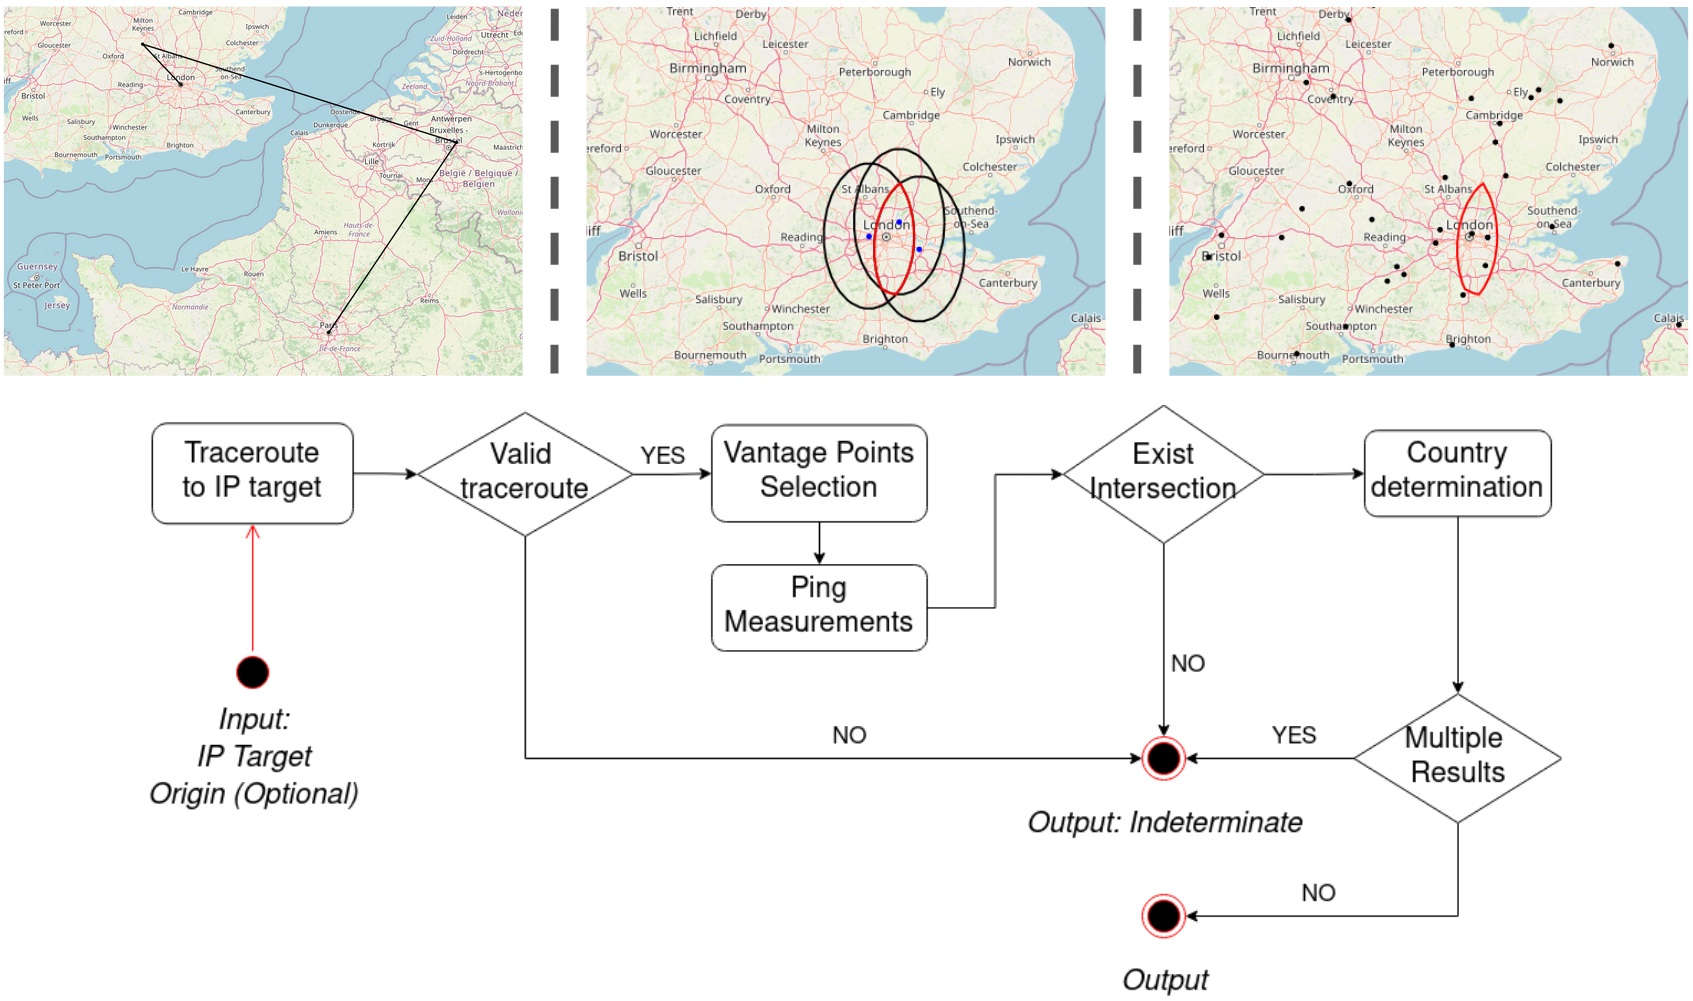
\includegraphics[width=\textwidth]{figures/images/hunter_flow_with_map.png}
    \caption{Hunter methodology for determining the destination country of anycast communications.}
    \label{fig:hunter_flow_with_map}
\end{figure}

% ============================================================
\section{Tracing the Anycast Path}
\label{sc:hunter_tracing_anycast_path}
% ============================================================

The first step of Hunter consists of analysing the routing path followed by packets towards the target infrastructure. Because multiple anycast replicas share the same destination IP address, the objective is to identify the network elements closest to the replica that serves the traffic from a given origin network.

To address this problem, Hunter analyses the routing path towards the anycast destination using traceroute measurements. The objective of this phase is not to fully reconstruct the end to-end topology, but rather to identify the network elements closest to the actual destination infrastructure. In particular, the methodology focuses on determining the last hop before the anycast replica, since this router provides valuable information regarding the geographic region where the destination is likely deployed. Although the exact physical location of the serving replica remains unknown, routers located near the edge of the destination infrastructure are expected to exhibit a strong geographic correlation with the final service location. Consequently, identifying these routers enables the methodology to constrain the set of possible geographic regions associated with the destination of the communication.

Hunter relies on RIPE Atlas to perform the active measurements required by the methodology. The characteristics of RIPE Atlas and other Internet measurement infrastructures were introduced in Section~\ref{sc:background_location_measurements_infraestructures}. The availability of geographically distributed probes enables Hunter to perform traceroute and latency measurements from multiple vantage points and infer the geographic destinations associated with anycast communications.

\subsection{Last Hop Identification}
\label{sc:hunter_tracing_anycast_path_last_hop_identification}

Hunter relies on traceroute measurements to analyse the path followed by packets towards the anycast destination. Traceroute operates by sending packets with progressively increasing Time-To-Live (TTL) values, forcing intermediate routers to generate ICMP 'Time Exceeded' responses when the TTL reaches zero. By collecting these responses, traceroute reveals the sequence of routers traversed by the communication path. The traceroute paths obtained are analysed to determine the routers located closest to the destination infrastructure.

One of the key assumptions underlying the proposed methodology is that the last hop is geographically close to the serving replica. Here, the last hop refers to the network element topologically closest to the serving replica along the observed traceroute path. Hunter therefore identifies the router that appears immediately before the destination IP address in the traceroute path and designates it as the \textit{last hop}. This router constitutes the primary reference point used to estimate the geographic region associated with the communication destination. The last hop is not necessarily geographically close to the serving replica, as the intermediate network infrastructure or routing characteristics may violate this assumption. In such cases, the distance constraints derived from the last hop may be less precise, which will reduce the accuracy of the subsequent multilateration step.

The rationale behind this assumption is that routers located near the edge of the destination infrastructure are commonly deployed within the same metropolitan area, Internet Exchange Point (IXP), or regional network environment as the serving replica. Although the exact internal topology of anycast providers generally remains unknown, the geographic distance between the last observable router and the destination infrastructure is typically significantly smaller than the overall end-to-end communication path. Consequently, the last hop provides a substantially more constrained geographic reference than the anycast IP address itself.

% ============================================================
\section{Multilateration}
\label{sc:hunter_multilateration}
% ============================================================

After identifying the last hop associated with the anycast communication, the methodology estimates the geographic region where the serving replica is likely deployed. This estimation is performed through multilateration techniques using latency measurements collected from geographically distributed vantage points.

The rationale behind this approach is that the latency observed between a probe and the destination imposes a physical constraint on the maximum distance that packets may have travelled. By combining latency-derived constraints from multiple probes, it becomes possible to delimit the geographic region compatible with all the observed measurements\cite{Cicalese2016Latency-BasedSets}.

Although these databases cannot reliably geolocate anycast addresses themselves, geographic information about network infrastructure elements such as routers and Internet Exchange Points can often be obtained from publicly available infrastructure datasets and measurement platforms \cite{RIPEIPmap, Candela2025UsingInfrastructure}. Such information is used in Internet measurement studies to associate routers and other infrastructure elements with geographic locations \cite{CAIDAITK}.

Once the reference region has been determined, a set of geographically distributed vantage points  located near the last hop are selected to perform active measurements towards the anycast destination. Each probe performs ping measurements to obtain the RTT to the target. The measured RTT values are subsequently transformed into geographic distance constraints. Assuming an upper bound on packet propagation speed, the RTT observed from a given probe defines the maximum distance between the probe and the serving replica. Consequently, each probe constrains the destination to a bounded geographic region centred around the probe location.

By combining the constraints obtained from multiple probes, the methodology estimates the overlapping geographic area that is compatible with all latency observations. This intersection region constitutes the estimated deployment area of the serving anycast replica.

\subsection{Distance Estimation}
\label{sc:hunter_multilateration_distance_estimation}

The conversion of RTT measurements into geographic distance constraints requires estimating the maximum physical distance that packets may have travelled between the probe and the destination infrastructure.

Assuming a maximum propagation speed close to the speed of light in optical fibre, the measured RTT can be transformed into an upper bound on the end-to-end communication distance. Since the RTT includes both forward and return propagation times, only half of the measured latency contributes to estimating the one-way distance between the probe and the destination.

Formally, the maximum distance associated with a vantage point can be estimated as follows:

\begin{equation*}
    d = (RTT/2) * (c/n)   
\end{equation*}

where $d$ represents the maximum distance between the probe and the destination, $RTT$ corresponds to the measured round-trip time, $c$ denotes the speed of light in vacuum, and $n$ is the refractive index of the optical fibre, \textit{1.468}.

In practice, Internet routing paths rarely follow geographically optimal trajectories. Routing policies, peering agreements, congestion, and traffic engineering decisions may introduce substantial detours that increase latency independently of physical distance. Consequently, the obtained distance estimations should not be interpreted as exact geographic distances but rather as upper-bound constraints limiting the possible location of the destination infrastructure.

The previous formulation assumes that the packets travel through optimal geographical paths at the maximum propagation speed supported by optical fibre. However, real Internet routing paths rarely satisfy these conditions. Routing policies, peering agreements, traffic engineering mechanisms, and physical infrastructure constraints often introduce significant path inflation, causing packets to traverse substantially longer distances than the direct geographic path between the source and destination.

\subsubsection{VerLoc Distance Approximation}
\label{sc:hunter_multilateration_distance_estimation_verloc}

To account for this behaviour, Hunter incorporates the approximation proposed by VerLoc \cite{Kohls2022VerLoc:Systems}. VerLoc empirically observed that the effective propagation distance travelled by Internet traffic is typically larger than the geographic great-circle distance between endpoints due to routing inefficiencies and network detours. Instead of assuming ideal propagation conditions, VerLoc introduces a correction factor that models the average inflation observed in operational Internet paths, providing a more realistic upper bound for latency-based geographic inference.

Hunter incorporates the option of using this approximation into the multilateration process to reduce the probability of overestimating the geographic region compatible with the observed RTT measurements. Consequently, the obtained multilateration regions better reflect the uncertainty introduced by real-world Internet routing behaviour while still maintaining sufficiently constrained geographic estimations for country-level inference.

Based on the empirical results presented by VerLoc, a logistic regression model was derived to approximate the relationship between RTT and geographic distance under realistic Internet routing conditions. Formally, the obtained relation can be expressed as:

\begin{equation*}
    RTT = \frac{2*d}{c*(0.0061699 * d^{0.480214} + 0.0497791)}
\end{equation*}

where $d$ represents the distance travelled, $RTT$ the measured Round-Trip Time, and $c$ the speed of light in a vacuum.

The resulting expression does not admit a closed-form analytic inverse that allows for the direct derivation of the distance from an observed RTT value. Consequently, distance estimation must be performed numerically by approximating the inverse relation through precomputed RTT-distance mappings.

Since the model itself constitutes an approximation of real Internet routing behaviour, the distance estimations obtained inherently introduce a certain degree of error. Nevertheless, the results shown in section \textit{6.2. Results} of the VerLoc paper \cite{Kohls2022VerLoc:Systems}, show that this approach provides substantially more realistic geographic constraints than ideal propagation models based solely on optical fibre transmission speed.

% ============================================================
\section{Country Determination}
\label{sc:hunter_country_determination}
% ============================================================

Once the multilateration phase produces a geographic region compatible with the observed latency constraints, the final stage of the methodology consists of determining the jurisdiction associated with the anycast communication.

The primary objective of Hunter is not to obtain precise coordinate-level geolocation, but rather to identify the country \DIFdelbegin \DIFdel{where the serving anycast replica is likely deployed. This distinction is particularly important in the context of data protection and international data transfers, where jurisdictional boundaries constitute the relevant element for regulatory compliance }\DIFdelend \DIFaddbegin \DIFadd{in which the last element of the IP-level connection towards the anycast address is located, whatever the nature of that element. Depending on how the service is deployed, this element may be the server that hosts the service or an intermediate element operated by the provider, such as a CDN edge proxy or a load balancer, as discussed in Section~\ref{sc:hunter_limitations_ingress}. Country-level attribution is the relevant granularity because jurisdictional boundaries are the element considered in data protection }\DIFaddend analyses.

The geographic regions obtained during the multilateration phase may vary substantially in size depending on the distribution of the probes, the routing behaviour, and the latency consistency. Consequently, an additional inference step is required to transform the estimated geographic area into a country-level attribution.

The proposed methodology is based on the observation that large-scale anycast infrastructures are typically deployed near major metropolitan and interconnection areas. This behaviour is common among Content Delivery Networks (CDNs), cloud providers, and distributed Internet services, whose infrastructures are frequently located close to Internet Exchange Points (IXPs) and major population centres. Inspired by previous work in the field \cite{Cicalese2016Latency-BasedSets}, Hunter therefore uses major airports as geographic references that approximate metropolitan regions where anycast replicas are likely to be deployed.

This assumption is also reinforced by the operational practices adopted by several large-scale providers. For example, some CDNs identify server locations using the IATA code of the nearest airport, effectively associating replicas with metropolitan airport regions.

Once the multilateration region has been obtained, Hunter searches for airports located within the estimated overlapping area. Three possible situations may occur. First, if a single airport is identified within the region, the associated city and country are directly assigned as the inferred destination of the communication. Second, if multiple airports are identified but all belong to the same country, the communication is attributed to that country. Although the exact metropolitan area may remain ambiguous, the jurisdictional inference remains valid because all candidate regions belong to the same national domain. Finally, if the overlapping area contains airports associated with multiple countries, the inference is classified as \textit{Indeterminate}. This conservative approach avoids assigning potentially incorrect jurisdictions when the geographic uncertainty region spans multiple national boundaries.

In certain cases, no airport may be located directly within the overlapping area. Under these conditions, Hunter computes the centroid of the estimated region and selects the nearest airport as a geographic reference. Although this approximation may introduce additional uncertainty, it enables the methodology to maintain a consistent jurisdictional inference process even when the multilateration region does not directly overlap a metropolitan reference point.

By prioritising conservative country-level attribution over precise coordinate estimation, Hunter minimises false positive geographic assignments while maintaining sufficient accuracy for the analysis of \DIFdelbegin \DIFdel{international data transfers }\DIFdelend \DIFaddbegin \DIFadd{cross-border communications }\DIFaddend and jurisdictional exposure in anycast communications.

% ============================================================
\section{Limitations}
\label{sc:hunter_limitations}
% ============================================================

The methodology proposed in this chapter relies on active Internet measurements, routing-path analysis, and latency-based geographic inference to estimate the destination jurisdictions associated with anycast communications. Although the validation results obtained \ref{sc:hunter_validation} demonstrate that Hunter provides reliable country-level inference under real-world conditions, the methodology is inherently affected by several limitations associated with measurements at the Internet-scale and operational routing infrastructures.

These limitations do not constitute implementation flaws specific to Hunter, but rather intrinsic constraints imposed by the decentralised and dynamic nature of the Internet. Consequently, Hunter incorporates conservative inference mechanisms designed to minimise incorrect jurisdictional attributions whenever sufficient confidence cannot be achieved.

\subsection{Traceroute Limitations}
\label{sc:hunter_limitations_traceroute}

Hunter relies on traceroute measurements to identify the last observable network element before the anycast destination. However, traceroute is affected by several well-known limitations that may reduce the visibility of the actual routing path.

First, traceroute can be used with UDP, ICMP, or TCP protocols, producing different behaviours depending on the protocol selected. The default and traditional protocol used is UDP. The packets sent with UDP are directed to a port, in the Linux implementation \cite{Traceroute8Page} 33434, which has no usage in the common network services deployed on the Internet. This type of packet could be filtered by firewalls, producing a path limited to the network element prior to the firewall. If ICMP packets are selected, then standard ICMP echo packets are used, the same as those used for ping. These packets could have an advantage over UDP, as ICMP packets could be less filtered by network elements, as they are used by the owners of these elements for diagnosis. However, some very restrictive organisations do not reply to this protocol, or the ICMP packets are discarded. Finally, when the TCP protocol is selected, packets are sent to destination port 80, the same as the one used for HTTP. Since the HTTP port is rarely filtered, these TCP packets are also not filtered. Although TCP could be the most convenient protocol, this is not true in all cases. Since the TCP option is used, the packets sent are treated as HTTP. Therefore, the routing could be different, with fewer intermediate network elements or network elements acting differently in various ways due to a quality of service policy, resulting in hidden network elements.

The different behaviours of the three protocols can be observed in the measurements shown in Figure~\ref{fig:hunter_traceroute_protocols_examples}. Although all measurements target the same destination from the same source network, the observable paths differ depending on the selected protocol. UDP and ICMP reach the destination at hop 14, whereas TCP reaches it at hop 7. The measurements also contain non-responsive hops, which indicate that the corresponding probes did not elicit a response rather than that the network element is necessarily absent from the forwarding path.

\begin{figure*}[t]
    \centering
    \begin{tikzpicture}[
    font=\scriptsize
]

% =========================================================
% UDP
% =========================================================

\node[tablebox, anchor=north west] (udp) at (0,0) {
    \begin{tabular}{c|l}
        \multicolumn{2}{c}{\textbf{UDP (default)}} \\[2mm]
        \textbf{Hop} & \textbf{Observed address} \\ \hline
        1  & 138.4.11.131 \\
        2  & 138.4.5.4 \\
        3  & 138.4.0.1 \\
        4  & 192.168.214.19 \\
        5  & \textcolor{red!70!black}{* * *} \\
        6  & 192.168.201.3 \\
        7  & 172.17.0.13 \\
        8  & 193.145.14.233 \\
        9  & 130.206.212.105 \\
        10 & 130.206.245.25 \\
        11 & \textcolor{red!70!black}{* * *} \\
        12 & \shortstack[l]{108.170.252.225\\108.170.252.213} \\
        13 & \shortstack[l]{142.250.232.11\\142.250.232.27} \\
        \textbf{14} & \textcolor{green!45!black}{\textbf{142.251.142.142}} \\
    \end{tabular}
};

\node[
    below=1mm of udp.south,
    text=red!70!black,
    align=center
] {No response at hop 5 an 11};

\node[
    above=1mm of udp.north,
    font=\small\bfseries
] {UDP};


% =========================================================
% ICMP
% =========================================================

\node[tablebox, anchor=north] (icmp) at (0.5\textwidth,0) {
    \begin{tabular}{c|l}
        \multicolumn{2}{c}{\textbf{ICMP (-I)}} \\[2mm]
        \textbf{Hop} & \textbf{Observed address} \\ \hline
        1  & 138.4.11.131 \\
        2  & 138.4.5.4 \\
        3  & 138.4.0.1 \\
        4  & 192.168.214.18 \\
        5  & \textcolor{red!70!black}{* * *} \\
        6  & 172.17.0.14 \\
        7  & 172.17.0.13 \\
        8  & 193.145.14.233 \\
        9  & 130.206.212.105 \\
        10 & 130.206.245.25 \\
        11 & \textcolor{red!70!black}{* * *} \\
        12 & 108.170.252.225 \\
        13 & 142.250.232.27 \\
        \textbf{14} & \textcolor{green!45!black}{\textbf{142.251.142.142}} \\
    \end{tabular}
};

\node[
    below=1mm of icmp.south,
    text=red!70!black,
    align=center
] {No response at hops 5 and 11};

\node[
    above=1mm of icmp.north,
    font=\small\bfseries
] {ICMP};


% =========================================================
% TCP
% =========================================================

\node[tablebox, anchor=north east] (tcp) at (\textwidth,0) {
    \begin{tabular}{c|l}
        \multicolumn{2}{c}{\textbf{TCP (-T)}} \\[2mm]
        \textbf{Hop} & \textbf{Observed address} \\ \hline
        1 & 138.4.11.131 \\
        2 & 138.4.5.4 \\
        3 & 138.4.0.1 \\
        4 & \shortstack[l]{192.168.214.18\\192.168.214.19} \\
        5 & \textcolor{red!70!black}{* * *} \\
        6 & 192.168.201.3 \\
        \textbf{7} & \textcolor{green!45!black}{\textbf{142.251.142.142}} \\
    \end{tabular}
};

\node[
    below=1mm of tcp.south,
    text=red!70!black,
    align=center
] {No response at hop 5};

\node[
    above=1mm of tcp.north,
    font=\small\bfseries
] {TCP};


% =========================================================
% Legend
% =========================================================

\node[
    below=13mm of icmp.south,
    font=\scriptsize,
    text=black!70,
    align=center
] {
    \textcolor{red!70!black}{\textbf{* * *}} = no response
    \qquad
    \textcolor{green!45!black}{\textbf{IP}} = destination reached
    \qquad
    Multiple addresses = different responses observed at the same hop
};

\end{tikzpicture}
    \caption{Comparison of traceroute measurements using UDP, ICMP, and TCP probes towards the same destination. The measurements exhibit different observable paths depending on the selected protocol.}
    \label{fig:hunter_traceroute_protocols_examples}
\end{figure*}

\begin{comment}
\begin{Verbatim}[
    breaklines=true,
    breakanywhere=true,
    fontsize=\small,
    frame=single
]
hugopascual@hp-shared:~$ sudo traceroute -T google.com
traceroute to google.com (142.251.142.142), 30 hops max, 60 byte packets
 1  swcdc30-polaris.dit.upm.es (138.4.11.131)  2.367 ms  2.733 ms  3.127 ms
 2  pfsense1.dit.upm.es (138.4.5.4)  0.145 ms  0.107 ms  0.163 ms
 3  r7000-ext.dit.upm.es (138.4.0.1)  0.491 ms  0.450 ms  0.461 ms
 4  192.168.214.18 (192.168.214.18)  0.755 ms  0.729 ms 192.168.214.19 (192.168.214.19)  0.749 ms
 5  * * *
 6  192.168.201.3 (192.168.201.3)  1.326 ms  1.653 ms  1.943 ms
 7  lcmada-ag-in-f14.1e100.net (142.251.142.142)  1.924 ms  1.598 ms  1.717 ms
hugopascual@hp-shared:~$ sudo traceroute google.com
traceroute to google.com (142.251.142.142), 30 hops max, 60 byte packets
 1  swcdc30-polaris.dit.upm.es (138.4.11.131)  2.420 ms  2.734 ms  3.150 ms
 2  pfsense1.dit.upm.es (138.4.5.4)  0.500 ms  0.456 ms  0.427 ms
 3  r7000-ext.dit.upm.es (138.4.0.1)  0.525 ms  0.547 ms  0.551 ms
 4  192.168.214.19 (192.168.214.19)  0.754 ms  0.829 ms  0.796 ms
 5  * * *
 6  192.168.201.3 (192.168.201.3)  3.165 ms  2.953 ms  3.038 ms
 7  172.17.0.13 (172.17.0.13)  1.294 ms  1.224 ms  1.501 ms
 8  193.145.14.233 (193.145.14.233)  1.507 ms  1.242 ms  1.250 ms
 9  redimadrid-ppal.ethtrunk14-103.ciemat.rt2.mad.red.rediris.es (130.206.212.105)  1.591 ms  2.231 ms  2.172 ms
10  ciemat-rt2.ethtrunk1.telmad.rt1.mad.red.rediris.es (130.206.245.25)  2.082 ms  2.868 ms  2.395 ms
11  * * *
12  108.170.252.225 (108.170.252.225)  4.232 ms  4.167 ms 108.170.252.213 (108.170.252.213)  2.073 ms
13  142.250.232.11 (142.250.232.11)  2.125 ms 142.250.232.27 (142.250.232.27)  2.083 ms 142.250.232.11 (142.250.232.11)  2.042 ms
14  lcmada-ag-in-f14.1e100.net (142.251.142.142)  3.276 ms  1.706 ms  1.733 ms
hugopascual@hp-shared:~$ sudo traceroute -I google.com
traceroute to google.com (142.251.142.142), 30 hops max, 60 byte packets
 1  swcdc30-polaris.dit.upm.es (138.4.11.131)  2.700 ms  3.139 ms  3.589 ms
 2  pfsense1.dit.upm.es (138.4.5.4)  0.138 ms  0.136 ms  0.134 ms
 3  r7000-ext.dit.upm.es (138.4.0.1)  0.503 ms  0.535 ms  0.533 ms
 4  192.168.214.18 (192.168.214.18)  0.803 ms  0.989 ms  0.987 ms
 5  * * *
 6  172.17.0.14 (172.17.0.14)  0.978 ms  0.838 ms  0.826 ms
 7  172.17.0.13 (172.17.0.13)  1.083 ms  0.845 ms  0.891 ms
 8  193.145.14.233 (193.145.14.233)  0.995 ms  0.872 ms  0.878 ms
 9  redimadrid-ppal.ethtrunk14-103.ciemat.rt2.mad.red.rediris.es (130.206.212.105)  1.557 ms  1.673 ms  1.663 ms
10  ciemat-rt2.ethtrunk1.telmad.rt1.mad.red.rediris.es (130.206.245.25)  2.253 ms  2.069 ms  2.003 ms
11  * * *
12  108.170.252.225 (108.170.252.225)  2.420 ms  3.589 ms  3.091 ms
13  142.250.232.27 (142.250.232.27)  2.425 ms  2.415 ms  2.435 ms
14  lcmada-ag-in-f14.1e100.net (142.251.142.142)  2.242 ms  2.236 ms  2.338 ms
\end{Verbatim}
\end{comment}

Second, modern Internet infrastructures frequently employ technologies such as MPLS tunnelling, Equal-Cost Multi-Path (ECMP) routing, and traffic load balancing mechanisms. These technologies may obscure the actual forwarding path followed by packets or produce different traceroute paths for packets belonging to the same communication flow. Additionally, these technologies, instead of obscuring the path, produce multipathing. This multipath situation occurs when multiple paths can be recognised in the traceroute, indicating that two anycast replicas were involved in the measurement. If this effect is produced, Hunter takes the different paths as distinct and analyses them separately.

These limitations may affect the identification of the actual last hop router before the anycast replica. In certain scenarios, the last observable hop may correspond to an upstream transit provider or an intermediate routing element located relatively far from the serving replica. Consequently, the geographic reference obtained from the traceroute analysis may not perfectly correspond to the physical location of the destination infrastructure.

To mitigate these effects, Hunter does not rely exclusively on traceroute observations for geographic attribution. Instead, traceroute information is combined with multilateration constraints obtained from geographically distributed measurements. Furthermore, paths exhibiting inconsistent or unreliable routing behaviour are conservatively discarded during the inference process.

\subsection{Latency-based Inference Limitations}
\label{sc:hunter_limitations_latency_inference}

The multilateration phase of Hunter relies on RTT measurements to estimate upper-bound geographic constraints for the location of the serving anycast replica. However, Internet latency is influenced by multiple factors beyond physical distance, introducing uncertainty into the geographic inference process.

In operational networks, packets rarely traverse geographically optimal paths. Routing policies, peering agreements, congestion avoidance mechanisms, and traffic engineering decisions frequently produce significant routing inflation, increasing the effective distance travelled by packets independently of the actual geographic separation between endpoints.

Additionally, RTT measurements include multiple delay components beyond propagation latency, including transmission delays, processing delays, queueing delays, and access-network overhead. Temporary congestion conditions may further increase latency variability, particularly in heavily utilised networks or long-distance international links.

The last-mile infrastructure associated with probes and destination networks can also introduce additional variability. Consumer broadband connections, mobile networks, or access technologies with heterogeneous performance characteristics may contribute non-negligible latency components unrelated to geographic distance.

To reduce the impact of these phenomena, Hunter uses the minimum RTT observed across repeated measurements, minimising the influence of transient queuing delays and temporary congestion conditions. Furthermore, the methodology incorporates the VerLoc approximation \cite{Kohls2022VerLoc:Systems}, which models the empirical inflation commonly observed in real Internet paths and produces more realistic geographic constraints than the ideal optical propagation assumptions.

Nevertheless, latency-derived distances should not be interpreted as exact geographic estimations. The obtained constraints only define upper-bound regions compatible with the observed communication latency. Consequently, Hunter does not attempt precise coordinate-level geolocation, but instead focuses on conservative country-level inference.

\DIFaddbegin \subsection{\DIFadd{IP-Level Endpoint versus Processing Location}}
\label{sc:hunter_limitations_ingress}

\DIFadd{Hunter traces the last element of the IP-level connection towards the anycast address, whatever that element is. When the service is delivered directly by the servers that announce the address, this element is the server itself. When the service relies on a cloud or CDN provider, this element is usually the first element of the provider's infrastructure that terminates the connection, which could not coincide in all cases with the place where the content of the communication is decrypted and processed. The relationship between both depends on how the service is deployed, as illustrated by the enforcement levels discussed in Section~\ref{sc:rcadns_enforcement}.
}

\DIFadd{In services built on layer-7 proxies, such as CDNs and application load balancers, the edge element that answers the anycast address terminates TLS in order to read each request. The country inferred by Hunter is then the first country in which the content is available in clear. However, the request may subsequently be forwarded to other locations, such as upper cache tiers or application backends, which cannot be observed from outside, so the inferred country constitutes a lower bound of the jurisdictions involved. In services built on layer-4 accelerators or load balancers, the edge element may forward the encrypted stream to an endpoint located elsewhere, where TLS is terminated. In that case, the inferred country is a place where only connection metadata, such as the client IP address, is handled, and the location where the content is decrypted remains unobserved.
}

\DIFadd{Since the configuration of a service is not visible from outside, Hunter cannot determine which of these situations applies to a given anycast address. Consequently, the results of Hunter must be interpreted as the country in which the IP-level connection terminates. The communications analysed in this thesis are HTTPS requests issued by applications and libraries to web APIs, which are typically served through layer-7 infrastructures, but this cannot be verified for each individual service.
}

\DIFaddend \subsection{Anycast Routing Dynamics}
\label{sc:hunter_limitations_anycast_routing_dynamics}

Anycast infrastructures inherently introduce substantial routing dynamics due to the distributed nature of their deployment model. Communications directed towards the same anycast IP address may reach different replicas depending on BGP policies, peering relationships, traffic engineering mechanisms, or transient network conditions.

As a consequence, nearby probes selected around the same last hop region may occasionally reach different anycast replicas despite their geographic proximity. Similarly, the destination associated with a given communication origin may vary over time due to routing updates, load redistribution, congestion management, or failures within the network infrastructure.

These behaviours may produce inconsistent multilateration constraints, excessively large overlapping regions, or the absence of valid geographic intersections altogether. Such situations are particularly frequent in highly distributed CDN infrastructures, where traffic engineering mechanisms dynamically optimise latency and load balancing across multiple regions.

Validation experiments \ref{sc:hunter_validation} illustrate the practical impact of these routing dynamics, particularly in Northern European countries such as Finland and Norway, where substantial variability in destination attribution was observed in repeated measurements.

Importantly, these situations do not necessarily indicate an incorrect operation of the methodology but rather reflect the intrinsic instability of the underlying anycast routing system. In practice, the geographic destination of an anycast communication may genuinely change over time depending on the operational state of the network.

To address these scenarios, Hunter deliberately prioritises conservative inference decisions over aggressive geographic attribution. When routing instability prevents the methodology from confidently associating the communication with a single jurisdiction, the result is classified as \textit{Indeterminate}. The objective of Hunter is therefore not to maximise the number of resolved destinations, but to minimise incorrect jurisdictional attributions.

\subsection{Geographic Uncertainty}
\label{sc:hunter_limitations_geographic_uncertainty}

The final stage of Hunter infers the destination jurisdiction associated with an anycast communication by analysing the multilateration region obtained from the latency measurements. However, this process is also affected by several sources of geographic uncertainty.

First, the methodology partially depends on commercial IP geolocation databases to estimate the location of the last hop router. Although the router infrastructure is generally more stable than the end-user or cloud-server addresses, geolocation databases may still contain outdated or inaccurate information. Inaccurate last hop geolocation may affect the selection of nearby vantage points and increase the uncertainty of the resulting multilateration region.

Second, Hunter approximates destination metropolitan areas using airport locations inspired by previous work \cite{Cicalese2016Latency-BasedSets}. Although this approach provides practical and scalable geographic references, airports do not necessarily correspond exactly to the physical location of the serving infrastructure. Large metropolitan regions may contain multiple datacenters distributed across tens of kilometres, introducing additional uncertainty into city-level inference.

Furthermore, certain multilateration regions may overlap multiple metropolitan areas or cross national borders. This situation is particularly relevant in densely interconnected regions, where cities may be geographically close despite being subject to different jurisdictional frameworks. Under these circumstances, small variations in latency measurements or routing behaviour may produce ambiguity regarding the final jurisdiction associated with the communication.

Consequently, Hunter does not attempt highly precise geographic attribution and instead focuses on determining the most likely country associated with the communication. When the obtained geographic constraints are insufficient to confidently associate the communication with a single jurisdiction, the methodology conservatively returns an \textit{Indeterminate} result rather than risking an incorrect country attribution.

These limitations highlight the inherent uncertainty associated with Internet-scale geographic inference. Nevertheless, the validation results \ref{sc:hunter_validation} demonstrate that, despite these constraints, Hunter provides sufficient\DIFaddbegin \DIFadd{ly}\DIFaddend  reliable country-level attribution \DIFdelbegin \DIFdel{capabilities }\DIFdelend to support large-scale analysis of \DIFdelbegin \DIFdel{international data transfers }\DIFdelend \DIFaddbegin \DIFadd{cross-border communications }\DIFaddend over anycast infrastructures.

% ============================================================
\section{Validation}
\label{sc:hunter_validation}
% ============================================================

The proposed methodology and its software implementation, Hunter, were validated under real-world Internet conditions in order to evaluate their capability to infer the geographic destination of anycast communications. Since the primary objective of Hunter is to determine the jurisdiction associated with a communication, the validation process focuses on country-level attribution rather than precise coordinate-level geolocation.

Validating anycast geolocation mechanisms presents an important challenge, as obtaining reliable ground-truth information regarding the serving replica is generally difficult in operational infrastructures. To address this problem, the validation process leverages specific Cloudflare services whose HTTP responses expose location-related metadata associated with the serving infrastructure, as illustrated in Figure~\ref{fig:hunter_cloudflare_cf_ray}.

\begin{figure}[t]
    \centering
    \resizebox{\linewidth}{!}{%
        \begin{tikzpicture}[
    >=Latex,
    font=\small
]

% ------------------------------------------------------------
% Client and anycast destination
% ------------------------------------------------------------

\node[endpoint, minimum width=25mm] (client)
    {Client\\(VPN / probe)};

\node[anycastip, right=25mm of client] (anycast)
    {Cloudflare\\Anycast IP\\104.16.123.96};

% ------------------------------------------------------------
% Cloudflare replicas
% ------------------------------------------------------------

\node[replica, right=32mm of anycast, yshift=17mm] (madrid)
    {Datacenter\\Madrid, Spain};

\node[replica, right=32mm of anycast] (paris)
    {Datacenter\\Paris, France};

\node[replica, right=32mm of anycast, yshift=-17mm] (newyork)
    {Datacenter\\New York, USA};

% ------------------------------------------------------------
% HTTP request
% ------------------------------------------------------------

\draw[bgppath]
    (client) -- (anycast);

\node[
    font=\footnotesize,
    text=blue!80!black,
    align=center
] at ($(client.east)!0.5!(anycast.west)+(0,5mm)$)
    {HTTP request};

% ------------------------------------------------------------
% Anycast routing
% ------------------------------------------------------------

\draw[replicaLink]
    (anycast.east) -- (madrid.west);

\draw[
    draw=green!50!black,
    line width=1.5pt,
    ->,
    >=Latex
]
    (anycast.east) -- (paris.west);

\draw[replicaLink]
    (anycast.east) -- (newyork.west);

\node[
    font=\footnotesize\bfseries,
    text=green!45!black,
    align=center
] at ($(anycast.east)!0.5!(paris.west)+(0,7mm)$)
    {Serving replica};

% ------------------------------------------------------------
% Anycast annotation
% ------------------------------------------------------------

\node[
    font=\footnotesize\itshape,
    align=center,
    text width=35mm
] at ($(anycast.south)+(0,-9mm)$)
    {Same anycast IP,\\multiple geographic replicas};

% ------------------------------------------------------------
% HTTP response
% ------------------------------------------------------------

\node[
    tablebox,
    minimum width=43mm,
    minimum height=15mm,
    align=left,
    right=20mm of paris
] (response) {
    \textbf{HTTP response}\\[1mm]
    \texttt{CF-RAY: 7ABC1234-MAD}
};

\draw[
    draw=green!50!black,
    line width=1.2pt,
    ->,
    >=Latex
]
    (paris.east) -- (response.west);

% ------------------------------------------------------------
% Ground truth
% ------------------------------------------------------------

\node[
    tablebox,
    below=8mm of response,
    text width=43mm,
    align=center
] (groundtruth) {
    \textbf{Ground truth}\\[1mm]
    \texttt{MAD} $\rightarrow$ Madrid
};

\draw[
    draw=black!55,
    ->,
    >=Latex
]
    (response.south) -- (groundtruth.north);

\end{tikzpicture}

    }
    \caption{Cloudflare anycast validation using the \textit{CF-RAY} response header as geographic ground truth.}
    \label{fig:hunter_cloudflare_cf_ray}
\end{figure}

In particular, two anycast IP addresses belonging to the Cloudflare CDN were selected as validation targets. The first address, 192.5.5.241, belongs to a root DNS service, while the second address, 104.16.123.96, serves Cloudflare's official website. HTTP responses from these services include the \textit{CF-RAY} header, which contains the IATA airport code associated with the Cloudflare datacenter \DIFdelbegin \DIFdel{handling the request. Since this code identifies the metropolitan region that serves the communication, it can be used as a reliable approximation of the actual }\DIFdelend \DIFaddbegin \DIFadd{processing the request, that is, the datacenter that terminates TLS and decrypts its content. In most cases, this is also the datacenter through which the request enters the Cloudflare network, so the header provides a reliable reference for the }\DIFaddend destination reached by \DIFdelbegin \DIFdel{traffic}\DIFdelend \DIFaddbegin \DIFadd{the communication}\DIFaddend .

\DIFaddbegin \DIFadd{However, both locations may occasionally differ. Cloudflare may forward individual connections at the transport layer from an overloaded datacenter to a nearby one with available capacity, where they are decrypted and processed \mbox{%DIFAUXCMD
\cite{CloudflareTrafficManager}}\hskip0pt%DIFAUXCMD
. In such cases, Hunter locates the ingress datacenter while the ground truth reports a different one, which typically results in a }\textit{\DIFadd{Negative}} \DIFadd{or }\textit{\DIFadd{Indeterminate}} \DIFadd{outcome even when Hunter has correctly located the ingress point. A }\textit{\DIFadd{Positive}} \DIFadd{outcome would only arise if an error in Hunter's inference happened to coincide with the country of the datacenter to which the connection was forwarded. The expected effect of these forwarding mechanisms on the measured precision is therefore downward, and each }\textit{\DIFadd{Positive}} \DIFadd{result indicates that the country inferred by Hunter coincides with the country in which Cloudflare decrypted the communication.
}

\DIFaddend For each validation experiment, Hunter was executed using one of the selected IP addresses as the target destination. Immediately before running Hunter, an HTTP request was sent to the destination service in order to retrieve the \textit{CF-RAY} header and obtain the corresponding ground-truth location. The inferred country produced by Hunter was then compared with the country associated with the airport code declared by Cloudflare.

To account for temporal variations in Internet routing, the validation measurements were repeated over multiple days and at different times of day. For each validation measurement set, the HTTP request and Hunter measurements were performed together from each selected VPN exit node and for both target IP addresses. A total of 45 measurement sets were conducted over the course of 17 days, covering different times of day. This repetition allowed the evaluation to capture changes in anycast routing conditions and to assess the consistency of Hunter's geographic inference across repeated observations.

Since one of the main goals of this thesis is to analyse \DIFdelbegin \DIFdel{compliance with GDPR requirements regarding international transfersof personal data}\DIFdelend \DIFaddbegin \DIFadd{the geographic exposure of personal-data communications in relation to the GDPR requirements on international transfers}\DIFaddend , the validation was intentionally designed around European jurisdictions rather than as a globally exhaustive evaluation. Therefore, the experiment was conducted from 29 countries belonging to the EEA. To emulate communications originating from different European jurisdictions, Proton VPN was used to establish VPN exit nodes in all except one EEA member state, Liechtenstein. For each selected country, the physical location of the VPN server used as the exit node was verified to be within the corresponding country, ensuring that the measurement traffic entered the Internet from the intended jurisdiction. Liechtenstein could not be included in the validation because Proton VPN did not provide an exit node in that country.

The use of a VPN is a clear limitation of the validation methodology, instead of directly using RIPE Atlas probes as measurement origins. Ideally, the traceroute and latency measurements performed by Hunter should be executed directly from distributed RIPE Atlas probes while simultaneously obtaining the HTTP headers returned by the target service in order to guarantee that both observations correspond to the exact same communication context and anycast replica.

However, during the development of this work, no mechanism was identified to retrieve the HTTP response headers associated with HTTP measurements executed from RIPE Atlas probes. In particular, although RIPE Atlas supports HTTP measurements, the platform does not expose the complete HTTP response information required to obtain the \textit{CF-RAY} header used as ground truth during the validation process.

Consequently, the validation required the execution of both the HTTP request and Hunter from the same controlled environment, which was achieved through the use of VPN exit nodes located in different EEA countries. Although this approach may introduce slight differences with respect to native residential or RIPE Atlas routing conditions, it guarantees that the ground-truth HTTP request and the Hunter measurements observe the same anycast routing behaviour at the time of execution.

\subsection{Validation Metrics}

The validation process evaluates Hunter according to three possible outcomes: \textit{Positive}, \textit{Negative}, and \textit{Indeterminate}.

A result is classified as \textit{Positive} when the country inferred by Hunter matches the country associated with the destination declared by the Cloudflare service. A result is classified as \textit{Negative} when Hunter assigns a different country than the one indicated by the target infrastructure. Finally, a result is classified as \textit{Indeterminate} when the methodology cannot confidently infer a single jurisdiction due to inconsistent routing behaviour, insufficient geographic constraints, or violations of the assumptions described in previous sections.

Two complementary evaluation metrics are used during the validation process: precision and accuracy.

Precision is defined as the ratio between the number of Positive results and the sum of Positive and Negative results:

\begin{equation*}
    Precision = \frac{Positive}{Positive + Negative}
\end{equation*}

Accuracy is defined as the ratio between the number of Positive results and the total number of obtained results, including Positive, Negative, and Indeterminate outcomes:

\begin{equation*}
    Accuracy = \frac{Positive}{Positive + Negative + Indeterminate}
\end{equation*}

This distinction is particularly important in the context of Hunter, because the methodology deliberately prioritises conservative inference decisions over aggressive geographic attribution. Consequently, returning an \textit{Indeterminate} result is considered preferable to assigning an incorrect jurisdiction, especially in scenarios involving legal compliance and international data transfer analysis.

\subsection{Results}

The validation experiment evaluated Hunter under real-world Internet conditions in 29 EEA countries and multiple measurements conducted over several days and at different times of day. Each campaign combined an HTTP request to the selected anycast destination, used to obtain the \textit{CF-RAY} header as ground truth, with the corresponding Hunter measurements executed from the same VPN exit server. Two Cloudflare anycast IP addresses were evaluated, namely 192.5.5.241 and 104.16.123.96. In total, the experiment consisted 2739 measurements distributed throughout the period from June 2023 to July 2023.

The results obtained indicate that Hunter provides highly reliable country-level inference for anycast communications under real-world Internet conditions. Across all evaluated measurements, Hunter achieved a precision of 97.67\% and an accuracy of 78.09\%. The complete distribution of Positive, Negative, and Indeterminate results is presented in Table~\ref{tab:hunter_validation_results}.

\begin{table}[ht]
    \centering
    \small
    \caption{Summary of Hunter validation results.}
    \label{tab:hunter_validation_results}
    \begin{tabular}{lr}
        \toprule
        \textbf{Metric} & \textbf{Hunter} \\
        \midrule
        Countries evaluated & 29 \\
        Measurements & 2,739 \\
        Positive results & 2,139 \\
        Negative results & 51 \\
        Indeterminate results & 549 \\
        Precision & 97.67\% \\
        Accuracy & 78.09\% \\
        \bottomrule
    \end{tabular}
\end{table}


The results demonstrate that Hunter successfully minimises incorrect country attributions while still identifying the geographic destination of a substantial proportion of communications. The difference between precision and accuracy reflects the conservative nature of the methodology, which intentionally prioritises soundness over completeness by returning \textit{Indeterminate} results whenever sufficient confidence cannot be achieved.

The proposed methodology deliberately favours conservative inference decisions that minimise false positives, even if certain \DIFdelbegin \DIFdel{transfers }\DIFdelend \DIFaddbegin \DIFadd{communications }\DIFaddend remain unresolved. This design choice is particularly important in the context of privacy analysis and legal compliance assessment, where incorrectly assigning a communication to a jurisdiction may lead to erroneous conclusions regarding international data transfers. Consequently, unresolved cases are retained rather than assigned to a geographic destination without sufficient supporting evidence.

A detailed analysis of the Negative results reveals that 94.12\% of all incorrect attributions, corresponding to 48 out of 51 cases, are concentrated in Norway and Finland. Hunter achieves country-level precisions of 50.72\% and 80.28\% in these two countries, respectively. These results suggest that the routing behaviour observed from some Northern European networks introduces greater instability in the geographic association between measurement origins and anycast replicas. The distribution of Positive, Negative, and Indeterminate results for each country evaluated is presented in Table~\ref{tab:hunter_validation_results_country}.

Additionally, the experiments showed that repeated measurements over time can mitigate these inconsistencies. When considering the complete set of destination countries inferred for each source, no incorrect attributions were observed in the scenarios evaluated. However, individual measurement paths may still produce negative or erroneous results. For this analysis, destination countries accounting for less than 5\% of the country-level results obtained by repeated executions were excluded from the error calculation, as they were considered statistically unstable.

\begin{table}[ht]
    \centering
    \small
    \caption{Distribution of Hunter validation results by country.}
    \label{tab:hunter_validation_results_country}
    \begin{tabular}{lrrrr}
        \toprule
        \textbf{Country} & \textbf{Measurements} & \textbf{Positive} & \textbf{Negative} & \textbf{Indeterminate} \\
        \midrule
        Austria & 56 & 49 & 0 & 7 \\
        Belgium & 112 & 57 & 0 & 55 \\
        Bulgaria & 112 & 102 & 0 & 10 \\
        Croatia & 110 & 97 & 0 & 13 \\
        Cyprus & 111 & 105 & 0 & 6 \\
        Czech Republic & 88 & 63 & 0 & 25 \\
        Denmark & 110 & 85 & 0 & 25 \\
        Estonia & 110 & 102 & 0 & 8 \\
        Finland & 110 & 57 & 14 & 39 \\
        France & 110 & 102 & 0 & 8 \\
        Germany & 112 & 89 & 0 & 23 \\
        Greece & 110 & 105 & 0 & 5 \\
        Hungary & 110 & 97 & 0 & 13 \\
        Iceland & 67 & 53 & 0 & 14 \\
        Ireland & 110 & 100 & 1 & 9 \\
        Italy & 110 & 73 & 1 & 36 \\
        Latvia & 110 & 84 & 0 & 26 \\
        Liechtenstein & \textit{N/A} & \textit{N/A} & \textit{N/A} & \textit{N/A} \\
        Lithuania & 100 & 59 & 0 & 41 \\
        Luxembourg & 80 & 28 & 1 & 51 \\
        Malta & 86 & 76 & 0 & 10 \\
        Netherlands & 86 & 66 & 0 & 20 \\
        Norway & 86 & 35 & 34 & 17 \\
        Poland & 86 & 61 & 0 & 25 \\
        Portugal & 45 & 40 & 0 & 5 \\
        Romania & 86 & 75 & 0 & 11 \\
        Slovakia & 86 & 76 & 0 & 10 \\
        Slovenia & 86 & 67 & 0 & 19 \\
        Spain & 110 & 97 & 0 & 13 \\
        Sweden & 44 & 39 & 0 & 5 \\
        \midrule
        \textbf{Total} & \textbf{2,739} & \textbf{2,139} & \textbf{51} & \textbf{549} \\
        \bottomrule
    \end{tabular}
\end{table}


\subsection{Cross-border Communications during Validation}

The communications observed during the validation process already reveal a significant number of \DIFdelbegin \DIFdel{international data transfers }\DIFdelend \DIFaddbegin \DIFadd{cross-border communications }\DIFaddend associated with anycast infrastructures. Figure~\ref{fig:hunter_validation_flows} illustrates the communication flows obtained during the validation experiments targeting the IP address 192.5.5.241. Flows crossing the borders of the EEA are highlighted in red.

\begin{figure}
    \centering
    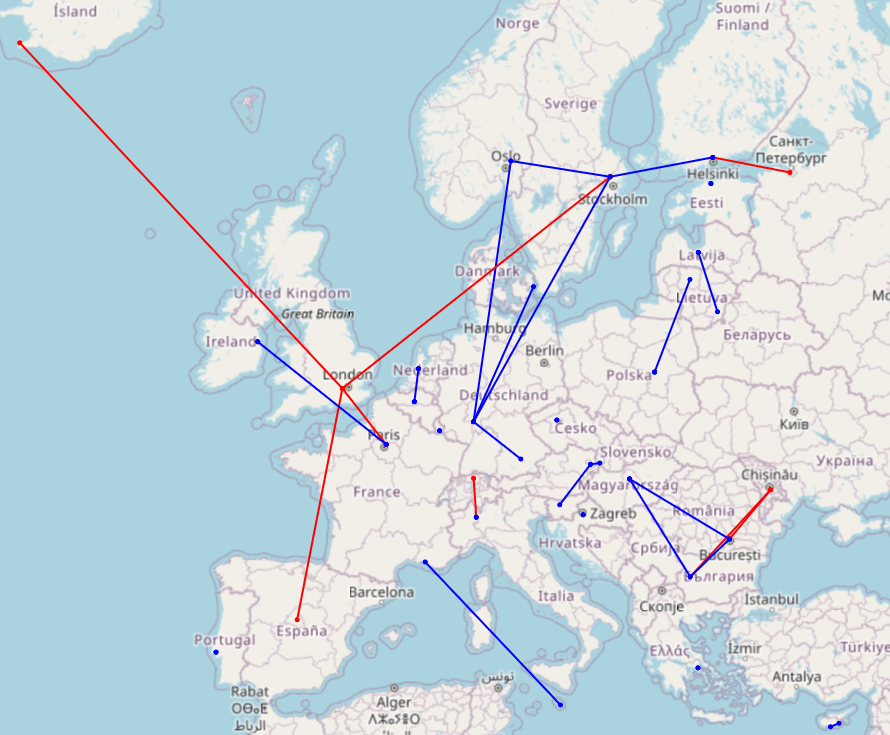
\includegraphics[width=\textwidth]{figures/images/hunter_validation_flows.png}
    \caption{Data flows obtained during Hunter validation for the target 192.5.5.241. Communications crossing EEA borders are highlighted in red.}
    \label{fig:hunter_validation_flows}
\end{figure}

The validation experiments identified multiple destination countries outside the EEA, including the United Kingdom, Switzerland, Moldova, and Russia. These observations confirm that anycast routing may direct communications towards jurisdictions outside the expected regulatory domain, even when the communication originates within the EEA.

During the experiments, three different patterns of \DIFdelbegin \DIFdel{international transfers }\DIFdelend \DIFaddbegin \DIFadd{cross-border communications }\DIFaddend were observed: recurrent, frequent, and episodic\DIFdelbegin \DIFdel{transfers}\DIFdelend .

Recurrent \DIFdelbegin \DIFdel{transfers }\DIFdelend \DIFaddbegin \DIFadd{patterns }\DIFaddend correspond to scenarios where communications from a given country systematically reach the same external jurisdiction. For example, communications originating from Spain and Iceland consistently reached servers located in the United Kingdom.

Frequent \DIFdelbegin \DIFdel{transfers }\DIFdelend \DIFaddbegin \DIFadd{patterns }\DIFaddend correspond to situations where multiple destination countries are repeatedly observed with significant frequency. This behaviour was particularly visible in Finland, where communications were almost equally distributed between Sweden and Russia, depending on the routing conditions at the time of measurement.

Finally, episodic \DIFdelbegin \DIFdel{transfers }\DIFdelend \DIFaddbegin \DIFadd{patterns }\DIFaddend correspond to occasional routing deviations observed only during specific measurements. Examples include communications from Italy reaching Switzerland or communications from Sweden reaching the United Kingdom.

These observations demonstrate that the geographic destination of anycast communications may vary substantially depending on transient routing conditions, traffic engineering decisions, and BGP dynamics. Consequently, determining the actual jurisdiction reached by a communication requires continuous observation and active measurement rather than relying exclusively on static infrastructure assumptions or conventional IP geolocation databases.

% ============================================================
\section{Summary and Next Steps}
\label{sc:hunter_summary}
% ============================================================

This chapter has presented Hunter, a methodology for inferring the country in which an anycast communication terminates. Hunter identifies the last hop before the anycast replica through traceroute analysis, constrains its location through latency-based multilateration from RIPE Atlas probes, and determines the destination country conservatively, returning an indeterminate result whenever the available evidence does not support a reliable attribution. The validation conducted in 29 EEA countries over 2,739 measurements yielded a precision of 97.67\% and an accuracy of 78.09\%, \DIFdelbegin \DIFdel{and already revealed }\DIFdelend \DIFaddbegin \DIFadd{It also showed that communications originating in the EEA may terminate in countries outside it, following }\DIFaddend recurrent, frequent, and episodic \DIFdelbegin \DIFdel{transfers towards countries outside the EEA}\DIFdelend \DIFaddbegin \DIFadd{patterns}\DIFaddend . Hunter and its validation have been published in the article \emph{Hunter: Tracing anycast communications to uncover cross-border personal data transfers} \cite{Pascual2024Hunter:Transfers}.

These results show that Hunter provides sufficiently reliable geographic inference to \DIFdelbegin \DIFdel{study international data transfers over anycast infrastructures, and that }\DIFdelend \DIFaddbegin \DIFadd{determine where the IP-level connection of anycast communications terminates, which is a necessary first step for assessing whether they may involve international transfers of personal data. They also show that, in the analysed infrastructures, }\DIFaddend the destination of these communications cannot be determined from static assumptions\DIFdelbegin \DIFdel{about the infrastructure}\DIFdelend . Building upon these capabilities, Chapter~\ref{ch:experiments} applies Hunter to the personal-data communications generated by Android applications and their Third-Party Libraries, compares the destinations reached with those disclosed in privacy policies, and extends the analysis to \DIFdelbegin \DIFdel{operational }\DIFdelend \DIFaddbegin \DIFadd{a broader set of }\DIFaddend anycast infrastructures worldwide.
 \newpage 
 \newpage \chapter{\DIFdelbegin \DIFdel{International }\DIFdelend \DIFaddbegin \DIFadd{Cross-Border Exposure of Personal }\DIFaddend Data \DIFdelbegin \DIFdel{Transfers }\DIFdelend in Anycast Communications}
\label{ch:experiments}

The previous chapter introduced Hunter, a methodology capable of inferring the geographic destinations of anycast communications through active network measurements and latency-based multilateration techniques. Although the validation results demonstrated the feasibility and reliability of the proposed approach, the actual impact of anycast infrastructures on data protection and data sovereignty remains an open question. In particular, it is necessary to assess whether the use of anycast can \DIFdelbegin \DIFdel{introduce regulatory compliance issues }\DIFdelend \DIFaddbegin \DIFadd{create situations that are relevant from a regulatory perspective, such as potential international transfers that are not disclosed to users, }\DIFaddend due to the geographic distribution of its serving replicas and the resulting uncertainty about the jurisdiction in which a communication is processed.

The mobile application environment constitutes a particularly suitable setting for analysing this phenomenon because it involves multiple actors, including application developers, third-party library providers, and external service providers, which may participate in the processing and transmission of user data. Modern smartphones continuously interact with cloud infrastructures and online services, many of which rely on anycast communications, to provide functionalities such as content synchronisation, analytics, advertising, authentication, notifications, and multimedia delivery. As a consequence, mobile devices generate a large volume of network communications involving multiple service providers and potentially different jurisdictions.

The Android platform is especially appropriate for this analysis due to its worldwide adoption, the openness of its application distribution model, and the extensive use of TPLs. TPLs are ubiquitous in Android applications and have been reported to account for more than 60\% of the application code on average \cite{Wang2017UnderstandingAnalysis}. Android applications therefore rarely operate as isolated software components and instead integrate external libraries and Software Development Kits (SDKs) to provide functionalities such as analytics, advertising, crash reporting, authentication, content delivery, or user tracking. These components may access user data and establish direct network connections to remote servers independently of the application's own functionality \cite{He2019DynamicLibraries}. Consequently, communications generated by TPLs may involve external service providers and infrastructures whose geographic location is not directly apparent from the application itself.

From a regulatory perspective, this lack of geographic transparency introduces substantial challenges. Modern privacy regulations such as the GDPR \cite{REGULATIONSRelevance} impose obligations regarding international transfers of personal data, including transparency requirements concerning transfers to third countries and the safeguards applicable to such transfers. However, anycast infrastructures fundamentally decouple logical service identifiers from physical geographic destinations. Consequently, the jurisdiction effectively reached by an anycast communication may differ from the geographic location disclosed by a service provider or from the location assumed by an application developer.

To understand the impact of anycast on communications in a software ecosystem, this chapter presents a large-scale empirical analysis of \DIFdelbegin \DIFdel{international data transfers }\DIFdelend \DIFaddbegin \DIFadd{cross-border personal-data communications }\DIFaddend performed through anycast infrastructures within the Android platform. Using Hunter as the core geographic inference mechanism, the study analyses the destinations reached by anycast communications generated by Android applications and their embedded TPLs. The objective is twofold. First, the chapter seeks to quantify the prevalence of \DIFdelbegin \DIFdel{international data transfers }\DIFdelend \DIFaddbegin \DIFadd{cross-border personal-data communications }\DIFaddend associated with anycast \DIFdelbegin \DIFdel{communications }\DIFdelend and characterise their geographic behaviour. Second, it evaluates whether the observed destinations are consistent with the geographic information disclosed in the application privacy policies and the transparency obligations established by the applicable data protection frameworks, particularly the GDPR.

The analysis is progressively structured. First, the experimental methodology used for traffic collection, privacy policy analysis, and geographic inference is presented. Next, the chapter analyses the existence of cross-border \DIFdelbegin \DIFdel{personal data transfers }\DIFdelend \DIFaddbegin \DIFadd{personal-data communications }\DIFaddend triggered by anycast \DIFdelbegin \DIFdel{communications }\DIFdelend in Android applications, including their temporal variability and the prevalence of destinations located outside the EEA. Afterwards, the observed destinations are compared against the countries declared in privacy policies in order to evaluate the consistency between observed communication behaviour and disclosed information. The role of TPLs as one of the main drivers of these communications is then analysed in detail. Finally, the chapter extends the discussion beyond the Android platform and presents a broader perspective on jurisdictional exposure in operational anycast infrastructures, motivating the need for deterministic geographic control mechanisms discussed in subsequent chapters.

% ============================================================
\section{Experimental Setting}
\label{sc:anycast_experiments_setting}
% ============================================================

This chapter applies the empirical methodology introduced in the thesis in Section~\ref{sc:introduction_methodology} to study the role of anycast infrastructures in \DIFdelbegin \DIFdel{international data transfers }\DIFdelend \DIFaddbegin \DIFadd{cross-border personal-data communications }\DIFaddend within the Android ecosystem. \DIFaddbegin \DIFadd{Throughout the chapter, the terms }\textit{\DIFadd{cross-border communication}}\DIFadd{, }\textit{\DIFadd{potential international transfer}}\DIFadd{, and }\textit{\DIFadd{potential transparency gap}} \DIFadd{are used as defined in Section~\ref{sc:background_privacy_international_data_transfers}, and the destination countries reported correspond to the last element of the IP-level connection, as inferred by Hunter (Section~\ref{sc:hunter_limitations_ingress}). }\DIFaddend The experimental study applies this methodology to observe anycast communications generated by Android applications and their embedded TPLs, infer the geographic destinations reached by these communications using Hunter, and compare the observed jurisdictions with the information disclosed in the corresponding privacy policies.

The experimental workflow combines dynamic traffic analysis, active network measurements, and automatic inspection of privacy policies to characterise both the technical and regulatory dimensions of the problem. Figure~\ref{fig:experiment_tpls_analysis_workflow} summarises the workflow followed throughout the experiments, from the selection and execution of Android applications to the identification of anycast communications, geographic inference, and comparison with the corresponding privacy disclosures.

\begin{figure}
    \centering
    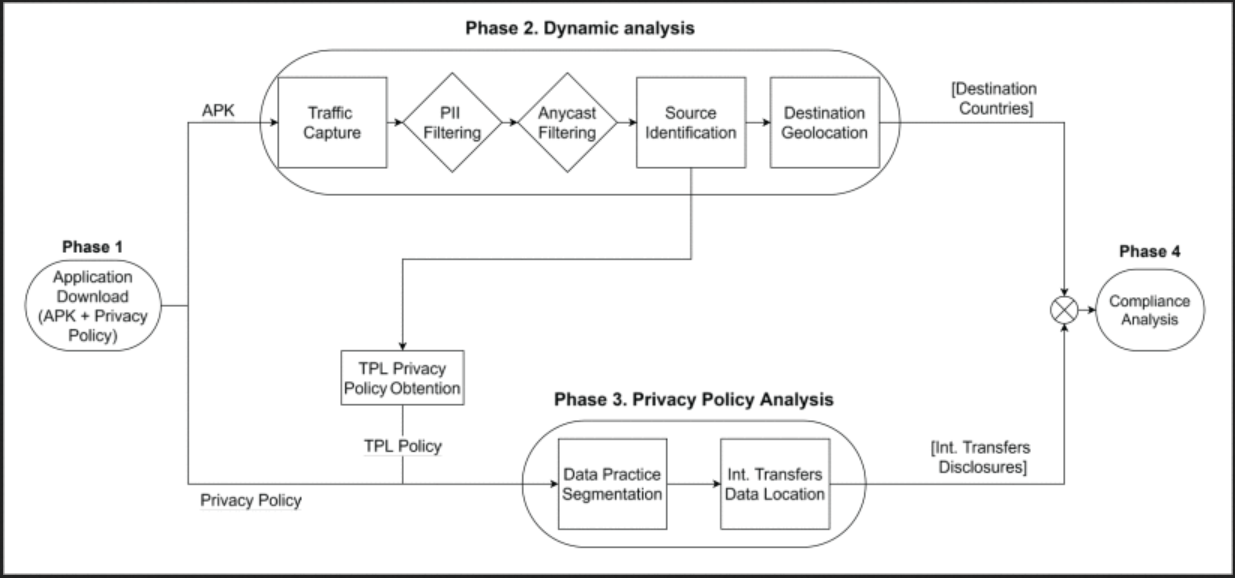
\includegraphics[width=\textwidth]{figures/images/experiment_tpls_analysis_workflow.png}
    \caption{Experimental workflow for analysing \DIFdelbeginFL \DIFdelFL{international data transfers }\DIFdelendFL \DIFaddbeginFL \DIFaddFL{cross-border personal-data communications }\DIFaddendFL in Android applications.}
    \label{fig:experiment_tpls_analysis_workflow}
\end{figure}

\subsection{Application Selection and Dataset Construction}
\label{sc:anycast_experiments_dataset}

The experimental analysis was conducted using a corpus of Android applications collected from the Google Play Store. We randomly selected 6,000 applications with more than 100,000 downloads \cite{Pascual2025AnycastDisaster}. The download threshold was used to focus the analysis on applications with a substantial user reach. The selected applications covered multiple categories of the Android platform, including communication, entertainment, productivity, finance, gaming, shopping, and social networking.

For each selected application, both the APK installation package and the associated privacy policy were automatically collected. The APK files were downloaded from the Google Play Store using the API described in \cite{Marty0678/googleplay-api:API}. Privacy policies were retrieved by scraping the corresponding application pages available on the Google Play Store, where developers are required to provide a policy link whenever personal data is processed.

Although 6,000 applications were initially selected, only 5,759 were processed successfully during the dynamic analysis phase. The remaining applications could not be executed successfully in the experimental environment due to anti-analysis protections, root detection mechanisms, execution failures, or incompatibilities with the instrumentation framework.

Dynamic analysis identified communications with external services associated with functionalities such as analytics, monetization, crash reporting, advertising, authentication, user tracking, and content delivery. These communications provide the basis for analysing the role of external services and TPLs in anycast traffic generated by Android applications. In particular, the presence of externally managed services creates communication paths whose geographic destinations may be determined by the underlying network infrastructure rather than directly by the application developer. This makes the Android application environment suitable for studying the geographic behaviour of anycast communications and its implications for \DIFaddbegin \DIFadd{potential }\DIFaddend international data transfers.

\subsection{Dynamic Traffic Analysis}
\label{sc:anycast_experiments_traffic_collection}

The second phase of the methodology focuses on executing the collected applications and analysing the network traffic generated during their operation in order to identify communications containing personal data and directed towards anycast infrastructures.

This phase is based on a previously developed framework and a combination of techniques for large-scale privacy analysis in Android applications \cite{Guaman2023AutomatedApplications}. The application execution environment, traffic interception infrastructure, execution trace collection mechanisms, and personal data identification techniques were inherited from this previous work. These components have also been evaluated and applied in previous experiments conducted by the research group \cite{Guaman2021GDPRApps,Jain2023ATLAS:Labels,Guaman2023AutomatedApplications,Pascual2024Hunter:Transfers,Rodriguez2024LargeScale}. Therefore, only the aspects directly relevant to the present study are summarised here.

The applications were executed on real Android devices within a controlled analysis environment. Each application was initially launched and was not interacted with for two minutes in order to capture its idle communications. Subsequently, the Android Monkey testing tool \cite{IUDevelopers} was used for three additional minutes to automatically stimulate the application and explore additional execution paths and communication behaviours.

During execution, the generated network traffic was intercepted through mitmproxy \cite{MitmproxyProxy}, a man-in-the-middle TLS interception proxy capable of inspecting HTTPS communications. This infrastructure enabled the extraction of destination domains, remote IP addresses, HTTP metadata, and application-layer payloads associated with the observed connections.

In parallel, an instrumentation component deployed on the Android devices collected execution traces from the running applications. These traces preserve package-level information regarding the code responsible for triggering each communication, enabling the identification of the embedded TPLs associated with the observed traffic.

The captured communications were then analysed to identify transmissions containing personal data based on the interpretation of personal data provided in the applicable European data protection guidelines \cite{JUSTICEwp260rev.01}. The detected personal data types include device identifiers, advertising identifiers, hardware information, operating system metadata, coarse and precise location information, and network information, such as WiFi BSSIDs to which the device is connected and MAC addresses.

The dynamic analysis intercepted a total of 4,278,823 communications generated by the analysed applications. Among them, 242,497 communications contained personal data. The collected traffic was subsequently filtered to retain only communications satisfying two simultaneous conditions: containing personal data and targeting anycast destination IP addresses. After applying these filters, the resulting dataset consisted of 195,786 communications directed towards 200 anycast IP addresses originating from 960 different Android applications \cite{Pascual2025AnycastDisaster}.

To determine whether a destination IP address belonged to anycast infrastructure, the methodology relied on publicly available datasets and commercial classification services, including the MAnycast2 census \cite{Sommese2020MAnycast2:Anycast} and the IPInfo commercial database \cite{IPIPinfo}. These sources provide information that enables the identification of operational anycast deployments. In particular, IPInfo explicitly annotates whether an IP address belongs to an anycast infrastructure, which enabled the filtering of communications directed towards anycast services during the analysis.

The execution traces additionally enabled the identification of embedded TPLs responsible for many of the observed communications. In total, 20 distinct TPLs were identified as triggering 61,443 communications containing personal data and directed towards anycast infrastructures.

As with any large-scale dynamic analysis methodology, the proposed approach presents inherent limitations. Dynamic execution cannot guarantee complete behavioural coverage, particularly for functionalities that require complex user interactions, authentication processes, or external conditions that may not be reproducible within the experimental environment. Consequently, the obtained results should be interpreted as a lower bound of the actual phenomenon rather than as an exhaustive enumeration of all possible communications performed by the analysed applications.

\subsection{Privacy Policy and Third-Party Library Analysis}
\label{sc:anycast_experiments_privacy_policies}

The third phase of the methodology focuses on analysing the privacy policies associated with both the Android applications and the embedded TPLs to evaluate the transparency of the observed international communications.

For each analysed application, the corresponding privacy policy text was automatically collected during the dataset acquisition phase. Subsequently, the policy texts were processed using machine learning and natural language processing techniques developed in previous work \cite{Guaman2023AutomatedApplications} to identify references related to international data transfers, third-party data sharing practices, and the countries where personal data may potentially be processed or accessed.

For each analysed application, the corresponding privacy policy text was automatically collected during the dataset acquisition phase. Subsequently, the policy texts were processed using machine learning and natural language processing techniques developed and evaluated in previous work \cite{Guaman2023AutomatedApplications}. In that previous evaluation, the supervised machine-learning classifier used to identify policy segments disclosing international data transfers achieved an F-measure of 90.9\%. Due to the class imbalance in the training corpus, the F-measure was prioritised over accuracy, and models with comparable F-measures were evaluated based on recall to favour a conservative identification of transfer disclosures. The subsequent identification of the countries to which personal data may potentially be transferred achieved an F-measure of 100\% for all countries except the United States, which achieved 99\% in the same evaluation. In the present study, these previously developed and evaluated techniques were applied to the privacy policies collected to identify references to international data transfers and the countries in which personal data may potentially be processed or accessed.

Particular attention was devoted to extracting the set of countries explicitly disclosed in the privacy policies as potential destinations for international personal data transfers. These disclosed jurisdictions were later compared against the actual geographic destinations of inferred anycast communications through Hunter.

The same analysis was conducted for the privacy policies associated with the identified TPLs. However, unlike application privacy policies, TPL privacy documentation frequently lacks standardised publication formats or consistent accessibility mechanisms. Consequently, the collection and verification of TPL privacy policies required partial manual intervention during the analysis process.

The analysis performed revealed a highly heterogeneous transparency landscape. Some applications explicitly disclosed destination countries and international transfer mechanisms, while many others provided generic references to international processing, cloud infrastructures, or external service providers without specifying the actual destinations countries of the observed communications.

A similar situation was observed among TPLs. Several libraries either lacked publicly accessible privacy policies or failed to explicitly identify the countries associated with their international data processing activities, despite generating communications towards anycast infrastructures located outside the EEA.

The comparison between the jurisdictions declared in privacy policies and the destinations empirically inferred through network measurements enabled the identification of applications and TPLs \DIFdelbegin \DIFdel{potentially failing to satisfy GDPR transparency requirements regarding }\DIFdelend \DIFaddbegin \DIFadd{whose privacy policies did not disclose the destination countries observed, which points to potential transparency gaps with respect to the GDPR requirements on }\DIFaddend international transfers of personal data.

\subsection{Anycast Destination Inference}
\label{sc:anycast_experiments_hunter_integration}

The final phase of the methodology focuses on determining the geographic destinations associated with the identified anycast communications. Since the destination reached by an anycast communication depends on the origin network and the dynamic state of Internet routing, identifying the physical location of the serving infrastructure requires active network measurements and geographic inference techniques. To address this problem, the experiments took advantage of Hunter, the methodology presented in Chapter~\ref{ch:hunter}. Hunter combines traceroute analysis, last-hop identification, latency-based multilateration, and country inference techniques to estimate the physical destination country associated with communications towards anycast infrastructures.

For each anycast IP address identified during the dynamic analysis phase, distributed measurements were executed from geographically distributed vantage points across the EEA using RIPE Atlas probes \cite{HomeAtlas}. The experiments focused on EEA countries because the GDPR establishes explicit transparency and adequacy requirements regarding international transfers of personal data outside the EEA jurisdictional space.

The source probes were selected by dividing the EEA territory into geographic cells of three degrees of latitude and longitude. For each cell, a random RIPE Atlas probe belonging to an EEA country was selected. \DIFdelbegin \DIFdel{Approximately 110 probes were used during each measurement campaign, providing broad geographic coverage across the EEA.
}%DIFDELCMD < 

%DIFDELCMD < %%%
\DIFdel{The source probes were selected by dividing the EEA territory into geographic cells of three degrees of latitude and longitude. For each cell, a random RIPE Atlas probe belonging to an EEA country was selected. }\DIFdelend Figure~\ref{fig:ripe_atlas_eea_mesh_cells} illustrates the geographic cells used for probe selection and the locations of the selected probes. Approximately 110 probes were used during each measurement during the campaign, providing broad geographic coverage across the EEA.

\begin{figure}[ht]
    \centering
    \includesvg[width=\textwidth]{figures/images/tpls_experiment_mesh_grid}
    \caption{Geographic cells used for RIPE Atlas probe selection.}
    \label{fig:ripe_atlas_eea_mesh_cells}
\end{figure}

For every source probe and anycast IP pair, Hunter inferred the destination country reached by the communication. The measurements were repeated 10 times for each IP in order to capture routing variability and identify potential changes in the selected anycast replica caused by network fluctuations, BGP routing dynamics, or traffic engineering mechanisms. 

The results produced by Hunter were subsequently combined with the traffic analysis and privacy policy datasets. This combination allowed us to identify the Android applications and TPLs that generated communications towards anycast infrastructures whose inferred geographic destinations were located outside the EEA. For these communications, the corresponding privacy policies were then analysed to determine whether the identified international destinations were transparently disclosed.

% ============================================================
\section{Cross-border Communications in Android Applications}
\label{sc:anycast_experiments_cross_border}
% ============================================================

\subsection{Observed Personal Information Anycast Communications}
\label{sc:anycast_experiments_observed_pii_anycast_communications}

The large-scale analysis of Android applications identified communications involving personal data that were directed towards anycast infrastructures. From the initial dataset of 6,000 applications, 5,759 were successfully analysed, generating a total of 4,278,823 network communications during the dynamic analysis phase.

Among these communications, 242,497 were identified as containing personal data according to the criteria described in Section~\ref{sc:anycast_experiments_traffic_collection}. The subsequent analysis of destination addresses identified communications directed towards anycast infrastructures. After filtering the collected traffic to retain only communications simultaneously containing personal data and targeting anycast IP addresses, the resulting dataset consisted of 195,786 communications, representing 80.74\% of all communications containing personal data, and involved 200 distinct anycast IP addresses.

These communications were generated by 960 different Android applications, corresponding to 16.67\% of the 5,759 applications successfully analysed. Table~\ref{tab:anycast_pii_apps_by_category} shows the number of applications generating personal-data communications towards anycast infrastructures for each Android application category. The observed communications were distributed across a wide range of application categories. Entertainment, Tools, Education, Puzzle, and Travel \& Local included the largest numbers of applications generating personal-data communications towards anycast infrastructures.

The identified communications involved several types of personal data, including device identifiers, advertising identifiers, hardware characteristics, operating system information, and location-related data. Table~\ref{tab:anycast_pii_communications_type} summarises the number and proportion of communications containing each identified personal data type. Advertising identifiers were the most frequently observed type, with Google Advertising IDs appearing in 74,162 communications (37.88\%), followed by device model information in 58,741 communications (30.00\%) and build information in 36,960 communications (18.88\%). Network-related information was also frequently observed, including WiFi BSSIDs in 18,790 communications (9.60\%). Location-related information appeared less frequently, with both precise and coarse device location identified in 312 communications (0.16\%) each.

\begin{table}[ht]
    \centering
    \small
    \caption{Personal data types identified in communications towards anycast infrastructures. Percentages are calculated with respect to the 195,786 communications containing personal data and targeting anycast IP addresses.}
    \label{tab:anycast_pii_communications_type}
    \begin{tabular}{lrr}
        \toprule
        \textbf{Personal data type} & \textbf{Communications} & \textbf{Percentage} \\
        \midrule
        Google Advertising ID & 74,162 & 37.88\% \\
        Device Model & 58,741 & 30.00\% \\
        Build Number & 36,960 & 18.88\% \\
        Router WiFi BSSID & 18,790 & 9.60\% \\
        Kernel Version & 4,152 & 2.12\% \\
        Router WiFi BSSID (Close) & 1,176 & 0.60\% \\
        Router WiFi MAC & 1,176 & 0.60\% \\
        Device Location & 312 & 0.16\% \\
        Coarse Device Location & 312 & 0.16\% \\
        Fingerprint & 5 & 0.00\% \\
        \midrule
        \textbf{Total} & \textbf{195,786} & \textbf{100.00\%} \\
        \bottomrule
    \end{tabular}
\end{table}

A more detailed breakdown of the personal data types observed across application categories is provided in Table~\ref{tab:anycast_pii_communications_category_type} in Appendix~\ref{ch:appendix_android_analysis}. This analysis shows how the different types of personal data were distributed across the application categories represented in the dataset, providing a more detailed characterisation of the data transmitted through communications towards anycast infrastructures.

These results characterise the types of personal data transmitted through communications towards anycast infrastructures and provide a quantitative basis for assessing the role of anycast in personal data transmission within Android applications.

\subsection{Temporal and Geographic Variability}
\label{sc:anycast_experiments_variability}

One of the most distinctive characteristics of anycast infrastructures is that the destination reached by a communication is not solely determined by the destination IP address. Instead, the selected server depends on the routing decisions made by the network, which are influenced by factors such as the geographic origin of the communication, BGP policies, peering agreements, traffic engineering mechanisms, and transient network conditions.

The measurements performed during the experiments confirmed that this behaviour is common among operational anycast deployments. For many of the anycast IP addresses analysed, communications originating from different EEA countries reached different destination countries despite targeting the same IP address. Consequently, the set of destinations potentially involved in an anycast communication cannot be determined solely from the destination address itself. Among the IP-origin pairs analysed, 74.8\% exhibited geographic variability, with communications from the same origin reaching more than one destination country. On average, each anycast IP address and source-origin pair reached 2.39 different destination countries.

In addition to geographic variability, the experiments also revealed temporal variability. Repeated executions of Hunter against the same anycast IP occasionally produced different destination countries even when the origin country remained unchanged. This behaviour reflects the dynamic nature of Internet routing, where modifications in network conditions, routing policies, congestion levels, or traffic engineering decisions may alter the anycast replica selected to serve a communication.

To capture this phenomenon, the destination inference process was repeated ten times for each source-destination pair. This repeated measurement strategy allowed the identification of different destination countries that may only appear under specific network conditions and reduced the risk of drawing conclusions from transient routing states. Furthermore, the same criterion used in the Hunter validation was applied to determine valid destination countries. A country was considered a valid destination if it represented more than 5\% of all measurements that produced a country-level destination. In this exact case, for each source-destination pair, the ten repetitions involved measurements from up to 110 different sources, resulting in up to 1,100 measurements.

\begin{figure}[ht]
    \centering
    \includesvg[width=\textwidth]{figures/images/ip_destination_countries_histogram}
    \caption{Distribution of the number of destination countries inferred for the analysed anycast IP addresses and source origins.}
    \label{fig:ip_destination_countries_histogram}
\end{figure}

The observed variability demonstrates that anycast infrastructures should not be understood as providing a single geographic destination. Instead, a communication directed towards an anycast IP address may potentially reach different countries depending on when and from where the communication is initiated. Figure~\ref{fig:ip_destination_countries_histogram} illustrates this variability by showing the distribution of the number of destination countries observed across the analysed measurements. Therefore, analysing only a single measurement or a single geographic origin would provide an incomplete view of the actual geographic exposure associated with anycast communications.

This behaviour has important implications for understanding the geographic footprint of anycast services. Rather than being associated with a single jurisdiction, many anycast deployments exhibit a set of potential destinations whose composition may vary over time, making the geographic behaviour of the service inherently dynamic.

\subsection{Destinations Outside the EEA}
\label{sc:anycast_experiments_non_eea}

After identifying the destination countries associated with the analysed anycast communications, the results were filtered to study \DIFdelbegin \DIFdel{those involving transfers of personal data towards }\DIFdelend \DIFaddbegin \DIFadd{the personal-data communications reaching }\DIFaddend countries located outside the EEA.

The analysis revealed that \DIFdelbegin \DIFdel{international transfers }\DIFdelend \DIFaddbegin \DIFadd{personal-data communications reaching countries }\DIFaddend outside the EEA were widely observed. Among the 200 anycast IP addresses identified during the experiments, 195 (97.5\%) were associated with at least one destination located outside the EEA. This indicates that communications carrying personal data towards anycast infrastructures may cross jurisdictional boundaries despite originating from users located within the EEA.

The inferred destinations outside the EEA included the United Kingdom, Switzerland, the United States, Ukraine, Serbia, and Russia. Figures~\ref{fig:transfers_outside_EEA}, \ref{fig:transfers_from_EEA_to_UK_and_SW}, and \ref{fig:transfers_from_EEA_to_RU_and_more} illustrate the geographical distribution of these \DIFdelbegin \DIFdel{transfers }\DIFdelend \DIFaddbegin \DIFadd{communications }\DIFaddend and the countries involved. \DIFaddbegin \DIFadd{These destinations differ in their regulatory situation: the United Kingdom and Switzerland benefit from an adequacy decision of the European Commission, and transfers to the United States can rely on an adequacy decision only when the recipient participates in the EU--US Data Privacy Framework, whereas Ukraine, Serbia, and Russia are not covered by any adequacy decision \mbox{%DIFAUXCMD
\cite{DataCountries}}\hskip0pt%DIFAUXCMD
. Reaching a non-EEA country does not by itself imply an unlawful transfer, but it exposes personal data to jurisdictions whose level of protection differs from that of the EEA. When no adequacy decision exists, such transfers require appropriate safeguards whose existence users cannot verify if the destination is not disclosed. Moreover, even when an adequacy decision exists, Article~13(1)(f) of the GDPR requires informing data subjects of the intention to transfer personal data to a third country and of the existence of that decision \mbox{%DIFAUXCMD
\cite{REGULATIONSRelevance}}\hskip0pt%DIFAUXCMD
, so these destinations remain relevant from the perspective of transparency.
}\DIFaddend 

For example, communications originating from Greece and Belgium were observed to reach Serbia through the anycast infrastructure associated with the IP address 104.17.45.20. Similarly, the IP address 188.114.96.5 produced 29 measurements in which communications originating from Finland reached Russia. These examples illustrate that the same anycast infrastructure may expose personal-data communications to jurisdictions outside the EEA and that the observed destination may depend on the geographic origin of the communication.

\begin{figure}
    \centering
    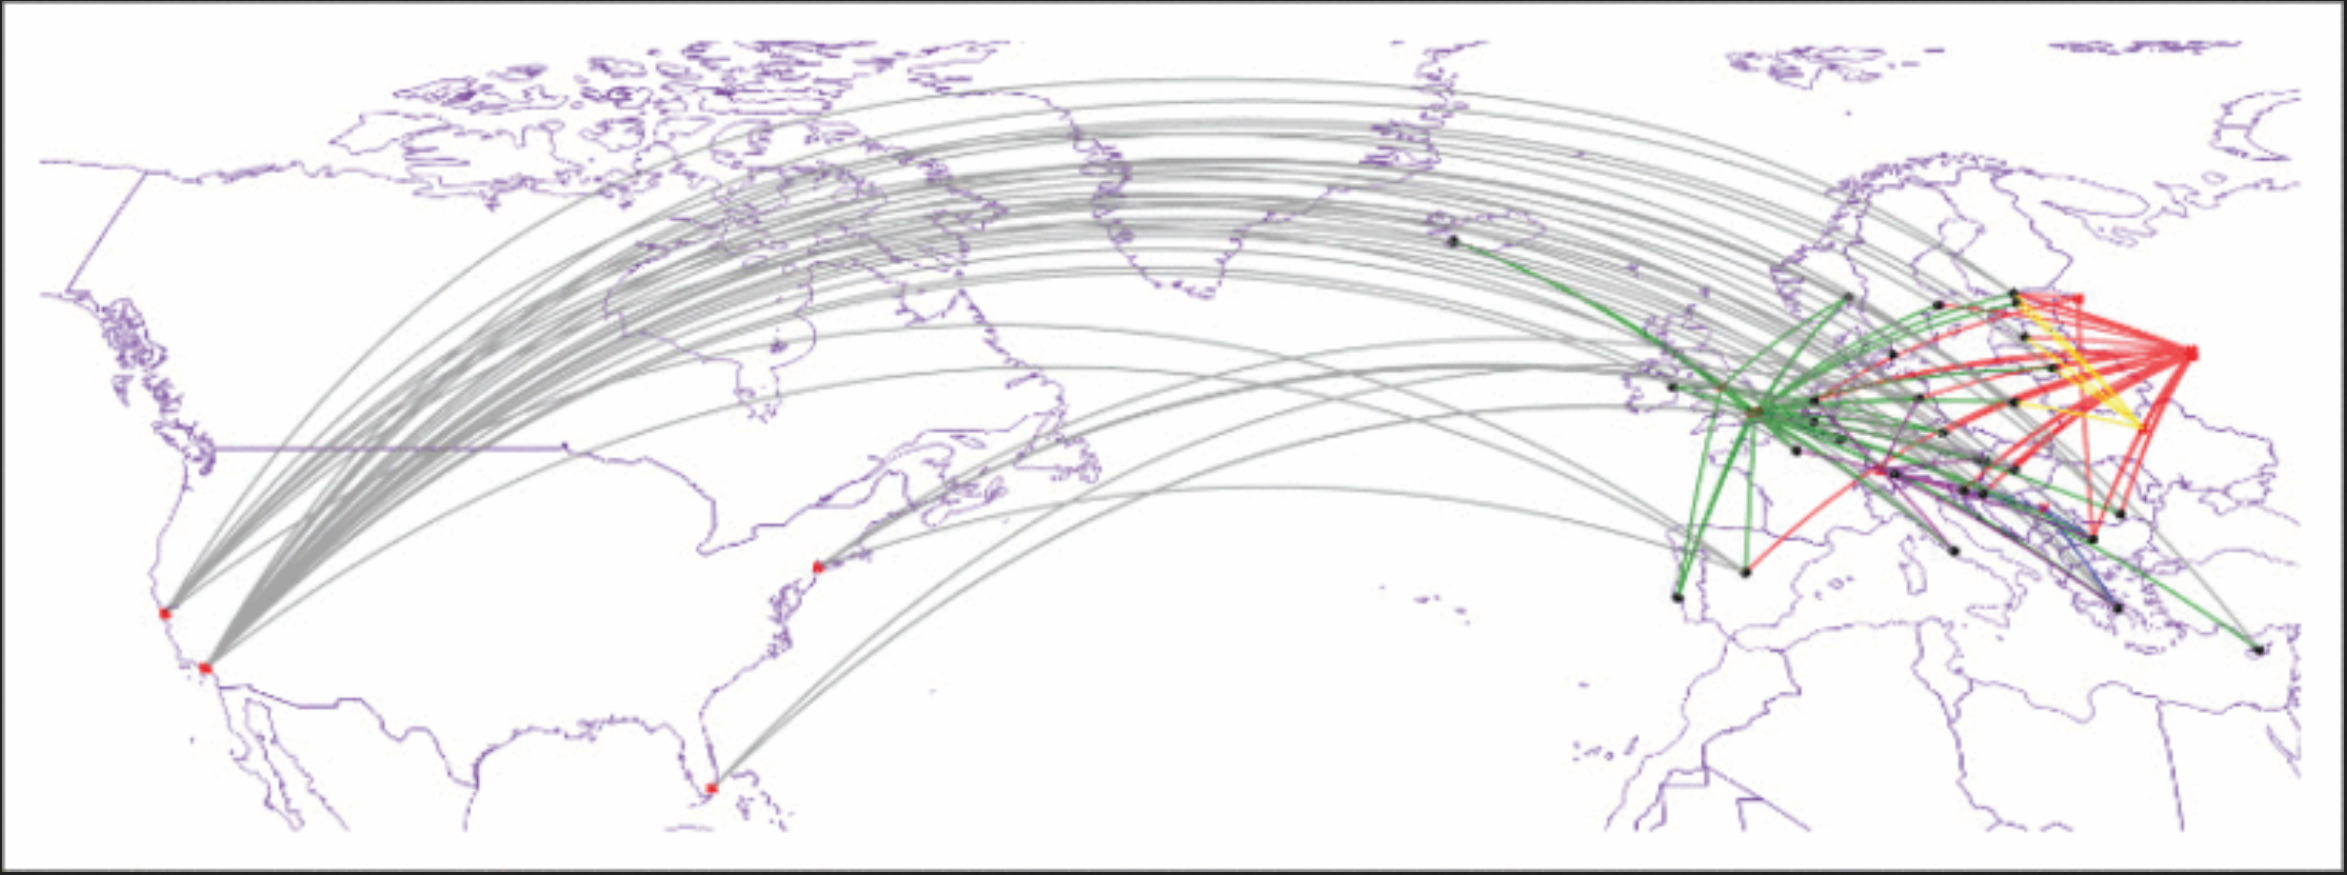
\includegraphics[width=\textwidth]{figures/images/transfers_outside_EEA.png}
    \caption{\DIFdelbeginFL \DIFdelFL{International transfers }\DIFdelendFL \DIFaddbeginFL \DIFaddFL{Personal-data communications }\DIFaddendFL from EEA countries \DIFdelbeginFL \DIFdelFL{to }\DIFdelendFL \DIFaddbeginFL \DIFaddFL{reaching }\DIFaddendFL non-EEA destinations.}
    \label{fig:transfers_outside_EEA}
\end{figure}

\begin{figure}
    \centering
    \begin{subfigure}[t]{0.48\textwidth}
        \centering
        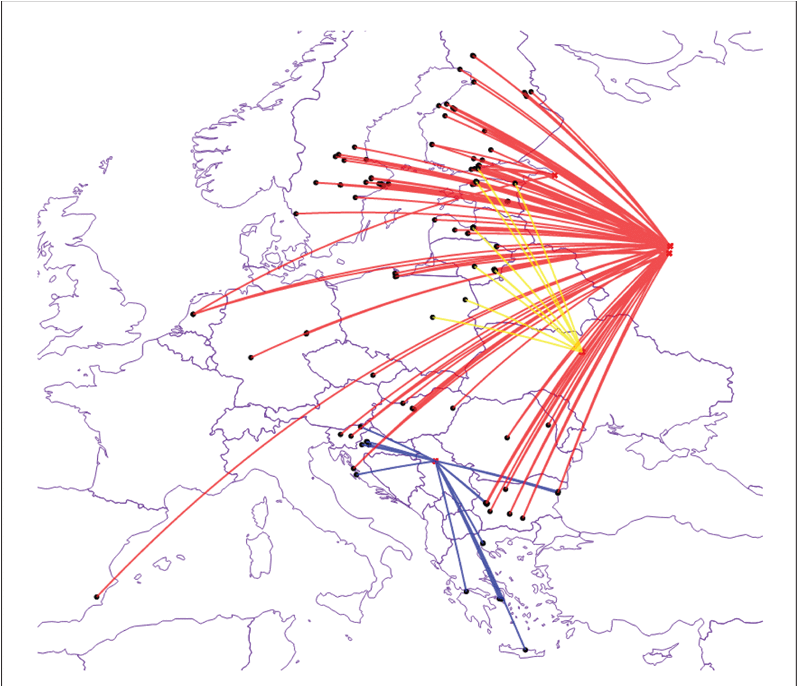
\includegraphics[width=\textwidth]{figures/images/transfers_from_EEA_to_RU_and_more.png}
        \caption{\DIFdelbeginFL \DIFdelFL{International transfers }\DIFdelendFL \DIFaddbeginFL \DIFaddFL{Communications }\DIFaddendFL from EEA countries \DIFdelbeginFL \DIFdelFL{to }\DIFdelendFL \DIFaddbeginFL \DIFaddFL{reaching }\DIFaddendFL anycast servers in Ukraine (yellow), Serbia (blue), and Russia (red).}
        \label{fig:transfers_from_EEA_to_RU_and_more}
    \end{subfigure}
    \hfill
    \begin{subfigure}[t]{0.48\textwidth}
        \centering
        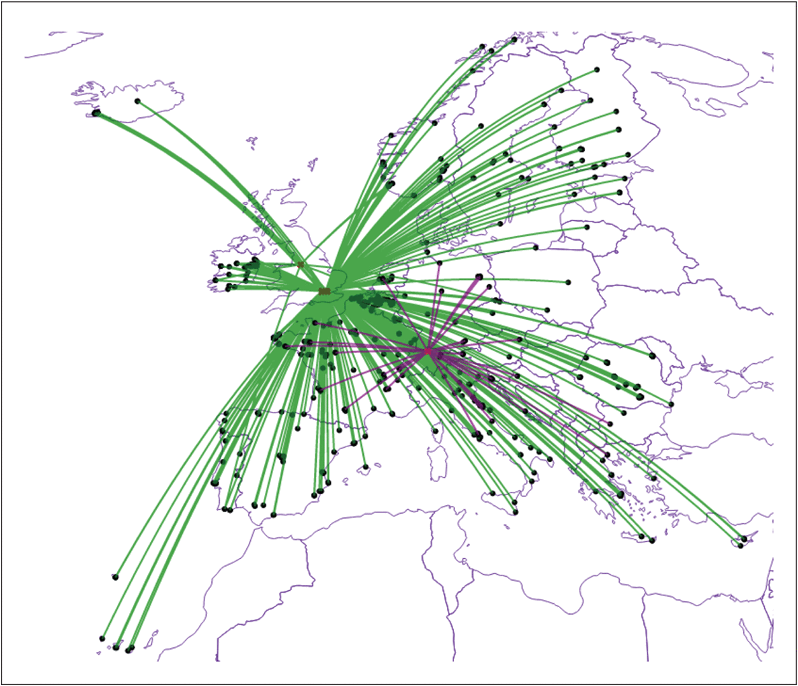
\includegraphics[width=\textwidth]{figures/images/transfers_from_EEA_to_UK_and_SW.png}
        \caption{\DIFdelbeginFL \DIFdelFL{International transfers }\DIFdelendFL \DIFaddbeginFL \DIFaddFL{Communications }\DIFaddendFL from EEA countries \DIFdelbeginFL \DIFdelFL{to }\DIFdelendFL \DIFaddbeginFL \DIFaddFL{reaching }\DIFaddendFL anycast servers in the United Kingdom (green) and Switzerland (purple).}
        \label{fig:transfers_from_EEA_to_UK_and_SW}
    \end{subfigure}
    \caption{\DIFdelbeginFL \DIFdelFL{International transfers }\DIFdelendFL \DIFaddbeginFL \DIFaddFL{Personal-data communications }\DIFaddendFL from EEA countries \DIFdelbeginFL \DIFdelFL{to }\DIFdelendFL \DIFaddbeginFL \DIFaddFL{reaching }\DIFaddendFL non-EEA destinations identified during the experiments.}
    \label{fig:transfers_non_eea}
\end{figure}

The results show that \DIFdelbegin \DIFdel{transfers towards }\DIFdelend \DIFaddbegin \DIFadd{communications reaching }\DIFaddend non-EEA countries were widely observed across the EEA. The United States and the United Kingdom were the most frequently observed non-EEA destinations, being reached from 80\% and 73.33\% of the EEA countries analysed, respectively. This behaviour is consistent with the geographic distribution of many anycast deployments, where traffic may be directed towards operational replicas located outside the user's jurisdiction, regardless of political or regulatory boundaries. The analysis also identified \DIFdelbegin \DIFdel{transfers towards }\DIFdelend \DIFaddbegin \DIFadd{communications reaching }\DIFaddend Russia, Switzerland, Ukraine, and Serbia. These observations demonstrate that geographic proximity alone cannot be assumed when reasoning about the destination of communications directed towards anycast infrastructures.

The results also revealed that the set of reachable destination countries varies depending on the origin country. The same anycast IP address can lead to different destination countries when accessed from different locations within the EEA, reinforcing the idea that anycast communications should be understood as a set of potential geographic destinations rather than a single fixed endpoint.

Overall, the results \DIFdelbegin \DIFdel{demonstrate that international transfers }\DIFdelend \DIFaddbegin \DIFadd{show that personal-data communications reaching countries }\DIFaddend outside the EEA were observed across a substantial fraction of the analysed anycast infrastructure and that the geographic exposure associated with these communications may extend beyond the jurisdictions where the applications themselves are distributed or executed.

% ============================================================
\section{Transparency \DIFdelbegin \DIFdel{and }\DIFdelend \DIFaddbegin \DIFadd{of }\DIFaddend Privacy \DIFdelbegin \DIFdel{Policy Compliance}\DIFdelend \DIFaddbegin \DIFadd{Policies}\DIFaddend }
\label{sc:anycast_experiments_transparency}
% ============================================================

\subsection{Undisclosed \DIFdelbegin \DIFdel{International Transfers}\DIFdelend \DIFaddbegin \DIFadd{Destination Countries}\DIFaddend }
\label{sc:anycast_experiments_undisclosed}

After identifying the destination countries reached by communications involving personal data, the next step consisted of comparing these empirically observed \DIFdelbegin \DIFdel{country }\DIFdelend destinations with the \DIFdelbegin \DIFdel{country destinations disclosed in the corresponding privacy policies. For each analysed application, the countries inferred through Hunter were contrasted with the list of destinations explicitly mentioned in the application's privacy policy. The same comparison was performed for the privacy policies of the TPLs identified as responsible for generating the observed communications.
}%DIFDELCMD < 

%DIFDELCMD < %%%
\DIFdel{After identifying the destination countries reached by communications involving personal data, the next step consisted of comparing these empirically observed destinations with the countries }\DIFdelend \DIFaddbegin \DIFadd{countries }\DIFaddend disclosed in the corresponding privacy policies. For the analysed applications, privacy policies were automatically collected from the Google Play Store during the dataset acquisition phase. For the TPLs, privacy policies were located and collected manually because their publication was not sufficiently uniform to support the same automated collection process. The privacy-policy analysis was then applied to applications using the machine-learning and natural language processing techniques described in previous work. In the case of TPLs privacy policies, the identification and categorisation of the disclosed destination countries were performed manually by the researchers.

For each analysed application, the countries inferred through Hunter were contrasted with the countries explicitly mentioned in the application's privacy policy. The same comparison was performed for the privacy policies of the TPLs identified as responsible for generating the observed communications.

Table~\ref{tab:anycast_tpls_privacy_destinations} summarises the TPLs identified in the experiment, the number of observed connections associated with each TPL, the availability of a privacy policy, the presence of the TPL in applications with more than 10 million downloads, the countries mentioned in their privacy policies, and the destination countries observed during the experiments. The table illustrates the discrepancy between the countries disclosed in the privacy policies and those empirically observed during the measurements. For example, BidMachine SDK for Android disclosed only the United States in its privacy policy, whereas communications associated with this TPL were observed reaching the United States, the United Kingdom, Russia, Ukraine, and Serbia. Similarly, Google Mobile Ads SDK did not disclose any specific country in the analysed policy, while communications associated with the library were observed reaching the United Kingdom, Switzerland, Russia, Ukraine, and Serbia.

\begin{table}[ht]
    \centering
    \footnotesize
    \setlength{\tabcolsep}{4pt}
    \caption{Third-Party Libraries associated with personal-data communications towards anycast infrastructures, their privacy-policy disclosures, and observed destination countries.}
    \label{tab:anycast_tpls_privacy_destinations}
    \begin{tabularx}{\textwidth}{>{\raggedright\arraybackslash}p{3.3cm} r r c c >{\raggedright\arraybackslash}X >{\raggedright\arraybackslash}X}
        \toprule
        \textbf{TPL} &
        \textbf{Apps} &
        \begin{tabular}[b]{@{}r@{}}\textbf{Connec-}\\\textbf{tions}\end{tabular} &
        \begin{tabular}[b]{@{}c@{}}\textbf{Privacy}\\\textbf{policy}\end{tabular} &
        \begin{tabular}[b]{@{}c@{}}\textbf{10M+}\\\textbf{apps}\end{tabular} &
        \textbf{Policy countries} &
        \textbf{Observed destinations} \\
        \midrule
        Unity Ads & 162 & 35,072 & Yes & 100--1000 & US, CA, JP, NZ, KR, CH, GB & GB, CH \\
        \rowsep{7}
        BidMachine SDK for Android & 7 & 9,200 & Yes & 10--100 & US & US, GB, RU, UA, RS \\
        \rowsep{7}
        Google Mobile Ads (GMA) SDK & 121 & 6,978 & Yes & 100--1000 & None & GB, CH, RU, UA, RS \\
        \rowsep{7}
        Adjust SDK & 55 & 3,470 & Yes & 100--1000 & None & US \\
        \rowsep{7}
        Appodeal SDK for Android & 14 & 3,127 & Yes & -- & US & GB, CH, RU \\
        \rowsep{7}
        Chartboost Monetization SDK & 11 & 1,068 & Yes & 10--100 & US & GB, CH \\
        \rowsep{7}
        MobSDK & 49 & 568 & No & -- & None & GB \\
        \rowsep{7}
        AdColony SDK & 29 & 430 & Yes & 10--100 & US & GB \\
        \rowsep{7}
        AppLovin SDK & 97 & 405 & Yes & 100--1000 & None & US, GB \\
        \rowsep{7}
        Kochava V4 & 6 & 278 & No & 1--10 & None & GB, CH \\
        \rowsep{7}
        OneSignal & 83 & 233 & Yes & 10--100 & US & GB, CH, RS \\
        \rowsep{7}
        bugsnag-android & 26 & 178 & Yes & 10--100 & US & GB \\
        \rowsep{7}
        New Relic Mobile for Android & 11 & 178 & Yes & 10--100 & None & US, GB, CH \\
        \rowsep{7}
        Official Mixpanel Android SDK & 8 & 85 & No & 10--100 & None & GB, CH \\
        \rowsep{7}
        Dynatrace OneAgent SDK & 1 & 73 & Yes & 10--100 & US & GB, UA \\
        \rowsep{7}
        Airship SDK & 3 & 38 & Yes & 10--100 & US, FR, DE, GB, SG, IN & GB \\
        \rowsep{7}
        Sentry Android & 3 & 32 & Yes & 10--100 & US, DE, CA & GB, CH, RU, RS \\
        \rowsep{7}
        EmarsysSDK & 2 & 16 & Yes & -- & None & GB \\
        \rowsep{7}
        Fyber FairBid SDK & 4 & 10 & No & 1--10 & None & GB \\
        \rowsep{7}
        Leanplum SDK FCM Module & 2 & 4 & Yes & 1--10 & US & GB \\
        \bottomrule
    \end{tabularx}
\end{table}

The distribution across applications was heterogeneous. Unity was associated with 162 applications, followed by AppLovin with 97 and OneSignal with 83, while several other TPLs were identified in fewer than ten applications. The number of applications associated with individual TPLs is not additive, as a single application may integrate multiple TPLs.

The comparison revealed a substantial discrepancy between the jurisdictions observed during the experiments and those disclosed to users. Although some privacy policies explicitly identified countries where personal data could be processed or transferred, many of the observed destination countries were not among those disclosed in the corresponding policies. For example, while the privacy policy of Sentry Android mentioned the United States, Germany, and Canada, communications associated with the library were observed reaching the United Kingdom, Switzerland, Russia, and Serbia. Conversely, Unity Ads was one of the cases in which the observed destinations, the United Kingdom and Switzerland, were also among the countries disclosed in its privacy policy.

In numerous cases, privacy policies described the use of cloud providers, content delivery networks, analytics services, or external partners without indicating the jurisdictions where these entities process data. As a result, the information available to users frequently lacked the geographic detail required to determine the countries that could receive personal data through anycast-enabled communications.

The discrepancy becomes particularly relevant in the context of anycast infrastructures. Since the destination of a communication may vary depending on the origin network and routing conditions, accurately disclosing all possible destination countries is considerably more challenging than in traditional unicast deployments. Nevertheless, from the perspective of the user, the practical consequence remains the same: \DIFdelbegin \DIFdel{personal data may be transferred to }\DIFdelend \DIFaddbegin \DIFadd{personal-data communications may reach }\DIFaddend jurisdictions that are not explicitly mentioned in the privacy documentation.

Among the applications \DIFdelbegin \DIFdel{identified as transferring personal data to }\DIFdelend \DIFaddbegin \DIFadd{whose personal-data communications reached }\DIFaddend anycast destinations located outside the EEA, 79.58\% did not explicitly mention international transfers in their privacy policies \cite{Pascual2025AnycastDisaster}. Among the TPLs policies, in some cases the policies only contained generic statements referring to international transfers of personal data without specifying the countries where personal data could ultimately be processed or no section about international transfers were present. These cases has been marked with a ``None'' in the \textit{Countries Mentioned in Policy} column of the Table\ref{tab:anycast_tpls_privacy_destinations}.

When the analysis focused specifically on destination countries, the discrepancy became even more pronounced. The results showed that 98.65\% of the analysed applications \DIFdelbegin \DIFdel{potentially failed to meet the GDPR transparency requirements regarding international transfers, as the }\DIFdelend \DIFaddbegin \DIFadd{did not adequately disclose in their privacy documentation the }\DIFaddend countries empirically observed during the experiments \DIFdelbegin \DIFdel{were not adequately disclosed in the corresponding privacy documentation \mbox{%DIFAUXCMD
\cite{Pascual2025AnycastDisaster}}\hskip0pt%DIFAUXCMD
}\DIFdelend \DIFaddbegin \DIFadd{\mbox{%DIFAUXCMD
\cite{Pascual2025AnycastDisaster}}\hskip0pt%DIFAUXCMD
. Since Article~13(1)(f) of the GDPR does not explicitly require naming each destination country, whereas the transparency guidelines of the Article~29 Working Party recommend doing so to the extent possible \mbox{%DIFAUXCMD
\cite{JUSTICEwp260rev.01}}\hskip0pt%DIFAUXCMD
, these results point to potential transparency gaps rather than to established non-compliance}\DIFaddend . The situation was similarly observed for TPLs. All identified TPLs \DIFdelbegin \DIFdel{were involved in }\DIFdelend \DIFaddbegin \DIFadd{generated }\DIFaddend personal-data \DIFdelbegin \DIFdel{transfers }\DIFdelend \DIFaddbegin \DIFadd{communications }\DIFaddend towards anycast infrastructures that could reach destinations outside the EEA. However, 90\% of these libraries \DIFdelbegin \DIFdel{potentially failed to }\DIFdelend \DIFaddbegin \DIFadd{did not }\DIFaddend disclose the corresponding destination countries despite \DIFdelbegin \DIFdel{actively participating in the international transfers }\DIFdelend \DIFaddbegin \DIFadd{generating the cross-border communications }\DIFaddend observed \cite{Pascual2025AnycastDisaster}.

The role of TPLs in these communications was also substantial. The 20 TPLs included in Table~\ref{tab:anycast_tpls_privacy_destinations} accounted for 61,443 observed connections, corresponding to 31.38\% of the 195,786 personal-data communications directed towards anycast infrastructures analysed in the experiment. This indicates that a substantial proportion of the observed communications involved functionality provided by embedded third-party components rather than application-specific infrastructure.

These findings indicate that users are frequently unable to determine the actual jurisdictions in which their personal data may be processed. Even when privacy policies acknowledge the possibility of international transfers, the information provided is often insufficient to identify the countries reached by the communications observed during the experiments. The results also suggest that the lack of transparency cannot be exclusively attributed to application developers. Since 31.38\% of the analysed personal-data communications towards anycast infrastructures were associated with the TPLs included in the analysis, deficiencies in transfer disclosures may propagate through the mobile ecosystem, affecting both application providers and third-party service operators.

\subsection{Limitations of Current Transparency Mechanisms}
\label{sc:anycast_experiments_transparency_limitations}

The observed discrepancies between the declared and actual destinations highlight a broader limitation of current transparency mechanisms when applied to modern Internet service infrastructures. Traditional privacy policies are generally written under the implicit assumption that the geographic location of data processing infrastructures is relatively stable and can, therefore, be described through a fixed list of countries or service providers. This assumption becomes increasingly difficult to maintain in environments that rely on anycast deployments.

Unlike conventional unicast infrastructures, anycast systems may route the same communication towards different physical locations depending on the origin network, routing policies, peering relationships, traffic engineering decisions, or temporary network conditions. As a result, the set of countries potentially involved in processing personal data may vary over time, even when users interact with the same service. This dynamic behaviour introduces a fundamental tension between technical reality and regulatory disclosure requirements. Privacy policies are static documents that are typically updated infrequently, whereas the geographic destinations reached through anycast routing may change continuously. Therefore, maintaining an exhaustive and accurate description of all possible destinations becomes operationally challenging. More importantly, this geographic uncertainty also challenges data sovereignty, as organisations cannot effectively control or guarantee the jurisdictions in which personal data is processed if the geographic destinations of their communications are not known or cannot be deterministically constrained. In this scenario, ensuring that personal data remain within a defined jurisdiction requires not only knowledge of the intended processing locations, but also effective control over the geographic destinations selected by the underlying network infrastructure.

The situation is further complicated by the widespread use of TPLs and external service providers. Application developers often rely on cloud platforms, analytics providers, advertising networks, and content delivery infrastructures that are managed by independent organisations. Consequently, developers may have limited visibility into the routing behaviour and geographic deployment strategies of the infrastructures that ultimately receive the data.

The results obtained in this study suggest that current transparency mechanisms are poorly adapted to highly distributed Internet architectures. Although privacy policies may disclose the existence of international transfers in general terms, they frequently fail to provide users with sufficient information to determine the jurisdictions that may actually receive their personal data. This limitation does not necessarily imply intentional non-compliance. Rather, it reflects the growing difficulty in reconciling legal transparency obligations with the dynamic and geographically distributed nature of contemporary Internet infrastructures. Nevertheless, from the perspective of users and regulators, the practical consequence remains unchanged: the actual destination countries of \DIFdelbegin \DIFdel{personal data transfers }\DIFdelend \DIFaddbegin \DIFadd{personal-data communications }\DIFaddend often remain unknown.

% ============================================================
\section{The Role of Third-Party Libraries}
\label{sc:anycast_experiments_tpls}
% ============================================================

The results presented so far show that \DIFdelbegin \DIFdel{international transfers }\DIFdelend \DIFaddbegin \DIFadd{cross-border personal-data communications }\DIFaddend through anycast infrastructures are widespread within the Android ecosystem. However, analysing the applications alone provides only a partial view of the phenomenon. A substantial fraction of the observed communications are not generated directly by the application code itself but by TPLs integrated into the applications.

Modern Android applications heavily rely on external libraries to provide functionalities such as analytics, advertising, crash reporting, authentication, social network integration, content delivery, and user tracking. Consequently, personal data transmitted by applications may be processed through infrastructures operated by organisations other than the application developer. Understanding the role of TPLs is therefore essential to determine how \DIFdelbegin \DIFdel{international data transfers }\DIFdelend \DIFaddbegin \DIFadd{cross-border personal-data communications }\DIFaddend emerge within mobile ecosystems and to identify the actors effectively responsible for the observed communications.

The execution traces collected during the dynamic analysis phase allowed the identification of the software components responsible for generating each observed communication. By analysing package names and execution contexts, it was possible to distinguish communications triggered directly by the application from those initiated by embedded TPLs. The results reveal a strong presence of third-party components in the analysed applications. In total, 20 different TPLs were identified as responsible for communications involving personal data and anycast infrastructures. These TPLs were associated with communications generated by 606 of the 960 applications that produced personal-data communications towards anycast infrastructures, corresponding to 63.13\% of the analysed applications. Table~\ref{tab:anycast_tpls_privacy_destinations} summarises the identified TPLs, together with the number of observed connections, their privacy-policy disclosures, and the destination countries observed during the experiments.

The widespread deployment of TPLs reflects the current structure of the mobile ecosystem, where application developers increasingly delegate specific functionalities to specialised external providers. Rather than implementing analytics, advertising, authentication, or telemetry systems internally, developers often integrate pre-built SDKs that offer these services through a simple programming interface. From a privacy perspective, this delegation has important implications. Although users typically interact with a single application, their personal data may be transmitted to multiple external organisations operating the embedded libraries, or used by them. As a result, understanding data flows within mobile ecosystems requires analysing not only the applications themselves but also the third-party components they incorporate.

The analysis revealed that TPLs play a central role in the generation of \DIFdelbegin \DIFdel{international personal data transfers }\DIFdelend \DIFaddbegin \DIFadd{cross-border personal-data communications }\DIFaddend through anycast infrastructures. Among the 195,786 communications involving personal data and anycast destinations identified during the experiments, 61,443 were directly attributed to embedded TPLs, corresponding to 31.38\% of the analysed communications. Furthermore, the geographic analysis performed using Hunter showed that all identified TPLs were involved in communications reaching destinations outside the EEA.

This observation is particularly relevant because the deployment strategies adopted by large cloud providers and Internet-scale platforms frequently rely on anycast infrastructures. As a result, a single SDK integrated into multiple applications may generate communications whose destinations vary dynamically depending on the geographic origin of the user and the state of the network. The findings therefore demonstrate that TPLs can play a substantial role in jurisdictional exposure within the Android ecosystem. Through their deployment across multiple applications, TPLs can generate communications whose geographic destinations vary according to the origin of the communication and the state of the network.

The prominent role of TPLs also raises important questions regarding responsibility and transparency in modern mobile ecosystems. From a technical perspective, application developers often have limited visibility into the internal operations of the libraries they integrate. Although developers may know the purpose of a given SDK, they may lack detailed information on the cloud infrastructures used by the provider, the geographic deployment of its services, or the routing mechanisms involved in processing user data.

Access to the privacy policies of TPL providers also presented practical difficulties. Unlike application privacy policies, which were collected automatically from the Google Play Store, TPL privacy policies had to be located and collected manually because their publication was not sufficiently uniform to support the same automated collection process. This lack of accessibility may further limit the ability of application developers to determine the data-processing and transfer practices disclosed by the providers of the libraries they integrate.

This lack of visibility becomes particularly problematic in the context of anycast infrastructures. Since the destination of a communication may depend on routing decisions that are external to both the application developer and the end user, accurately determining all potential destination jurisdictions becomes significantly more complex. The transparency analysis presented in the previous section illustrates this problem. Although all identified TPLs \DIFdelbegin \DIFdel{were involved in international transfers }\DIFdelend \DIFaddbegin \DIFadd{generated cross-border communications }\DIFaddend through anycast infrastructures, 90\% of them \DIFdelbegin \DIFdel{potentially failed to }\DIFdelend \DIFaddbegin \DIFadd{did not }\DIFaddend disclose the destination countries reached by these communications. As a consequence, application developers that integrate such libraries may also face difficulties in accurately informing users about the jurisdictions where their data may ultimately be processed.

These findings suggest that the transparency challenges associated with anycast infrastructures cannot be understood solely as an application-level problem. Instead, they emerge from the interaction between application developers, third-party service providers, cloud infrastructures, and Internet routing mechanisms. Consequently, improving transparency regarding international data transfers may require a broader ecosystem-wide approach in which both application developers and TPL providers participate in the disclosure process. Without greater visibility into the geographic behaviour of the infrastructures involved, accurately communicating the potential destinations of personal data transfers remains a challenging task for all actors in the mobile ecosystem.

% ============================================================
\section{Global Jurisdictional Exposure in Anycast Systems}
\label{sc:anycast_experiments_global_anycast}
% ============================================================

The previous sections analysed the geographic behaviour of anycast communications from the perspective of the EEA and demonstrated that personal-data communications generated by Android applications may reach destinations outside the region. To determine whether this behaviour is specific to the European context or reflects a broader property of operational anycast infrastructures, a second large-scale measurement campaign was conducted at a global scale.

The global experiment was conducted as an independent measurement campaign using a broader dataset of anycast infrastructures. A total of 489 anycast IP addresses were initially identified as candidates for the global analysis. Due to the time and measurement-credit constraints associated with the large-scale RIPE Atlas campaign, 195 of these IP addresses were analysed in the available measurement period. The analysed IP addresses were associated with 379 Android applications and were selected independently of the IP addresses analysed in the previous EEA-focused experiment. Consequently, the coincidence in the number of analysed IP addresses between the two experiments is incidental and does not indicate that the same infrastructures were analysed. The measurements were performed using Hunter from RIPE Atlas probes distributed across 183 countries. For each IP address, ten measurement rounds were conducted, with ten randomly selected probes per country in each round. Measurements were collected during two six-day periods in July and September 2025 at irregular intervals in order to capture variability in routing conditions over time.

After filtering incomplete traces and non-responsive paths, and applying the criterion of at least three origin-destination pairs for a valid observation, the campaign produced 504,690 valid routing tracks. Table~\ref{tab:global_hunter_summary} summarises the main characteristics of the dataset. The measurements covered 379 applications, 195 anycast IP addresses, and 183 countries. Of the valid routing tracks, 58.36\% terminated in a country different from the country of origin. Furthermore, 99.49\% of the analysed anycast IP addresses exhibited at least one cross-border routing event.

\begin{table}[ht]
    \centering
    \small
    \caption{Summary of the global anycast measurement campaign.}
    \label{tab:global_hunter_summary}
    \begin{tabular}{lr}
        \toprule
        \textbf{Metric} & \textbf{Value} \\
        \midrule
        Applications analysed & 379 \\
        Anycast IP addresses & 195 \\
        Countries covered & 183 \\
        Valid routing tracks & 504,690 \\
        Cross-border tracks & 58.36\% \\
        IP addresses with cross-border routing & 99.49\% \\
        \bottomrule
    \end{tabular}
\end{table}

Figure~\ref{fig:visualization_global_hunter} provides a global overview of the measurement campaign and illustrates the destinations observed for traffic originating in the United States, the EEA, and Japan. These examples demonstrate that cross-border routing is not confined to the European context analysed in the previous sections, but can also be observed from other major geographic regions.

\begin{figure}[ht]
    \centering
    \begin{subfigure}{0.48\textwidth}
        \centering
        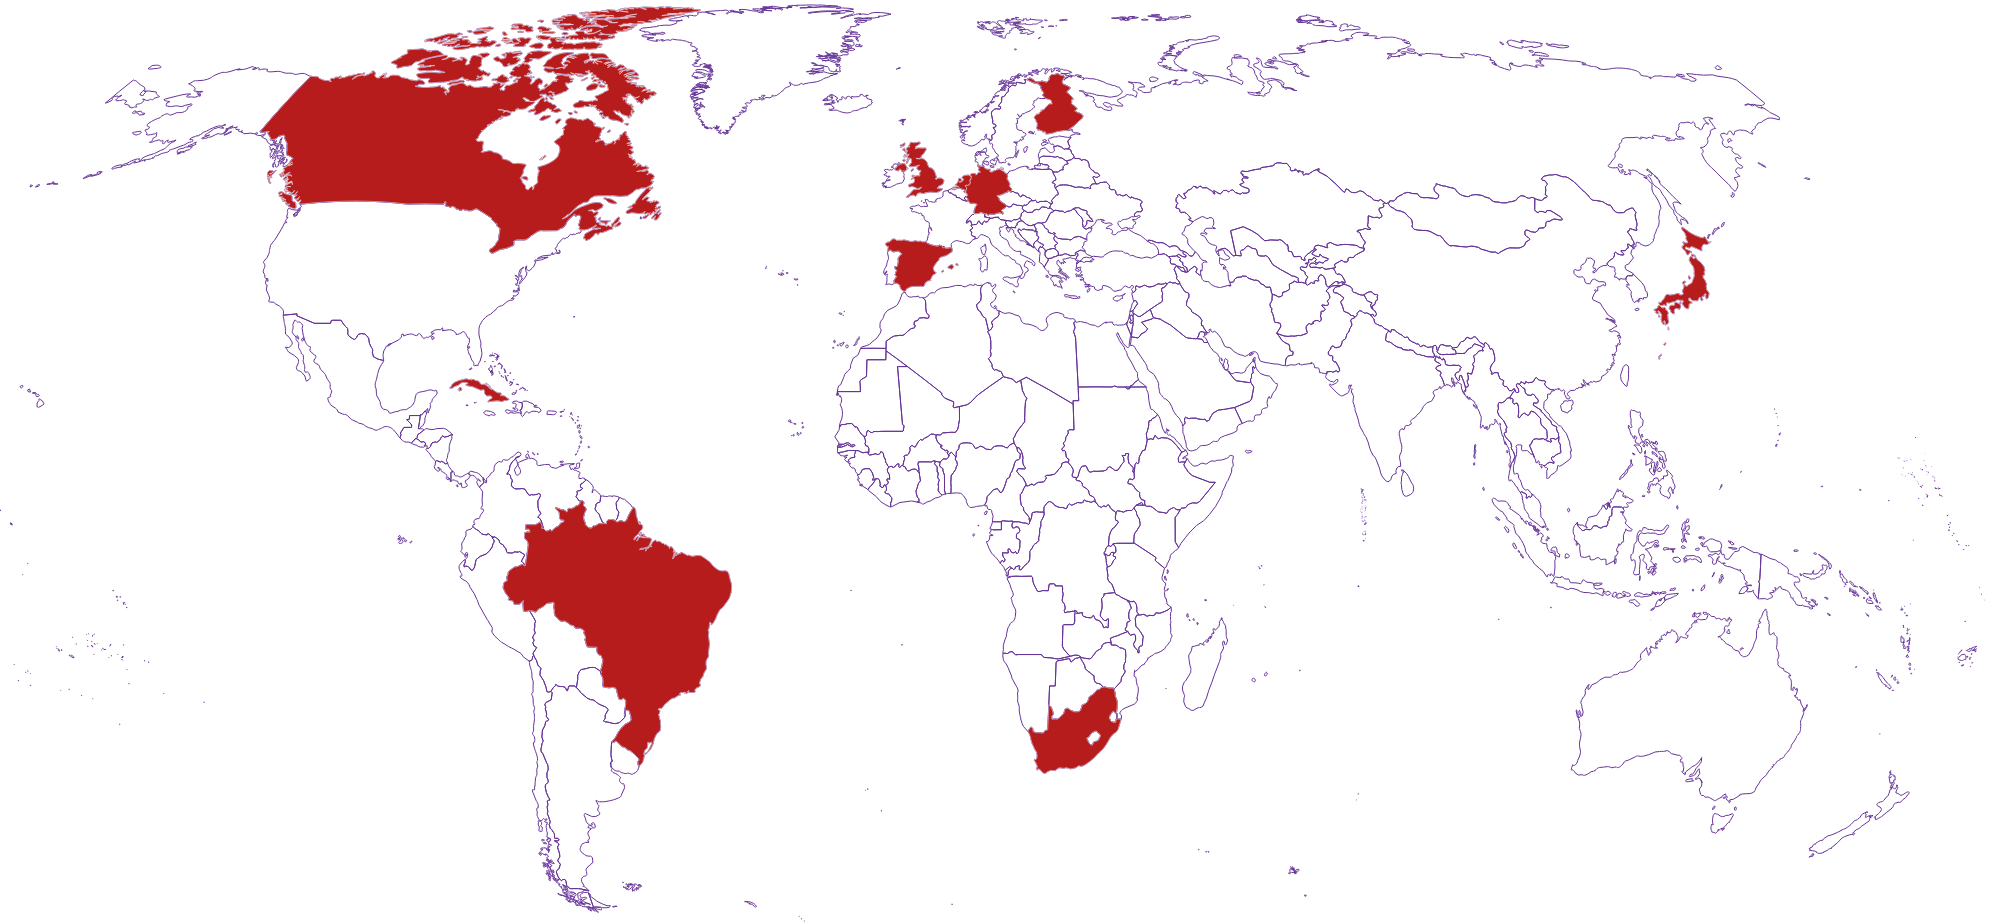
\includegraphics[width=\textwidth]{figures/images/figure_tracks_destinations_color_from_usa_no_scale.png}
        \caption{Destinations for traffic originating in the United States.}
        \label{fig:destinations_from_usa}
    \end{subfigure}
    \hfill
    \begin{subfigure}{0.48\textwidth}
        \centering
        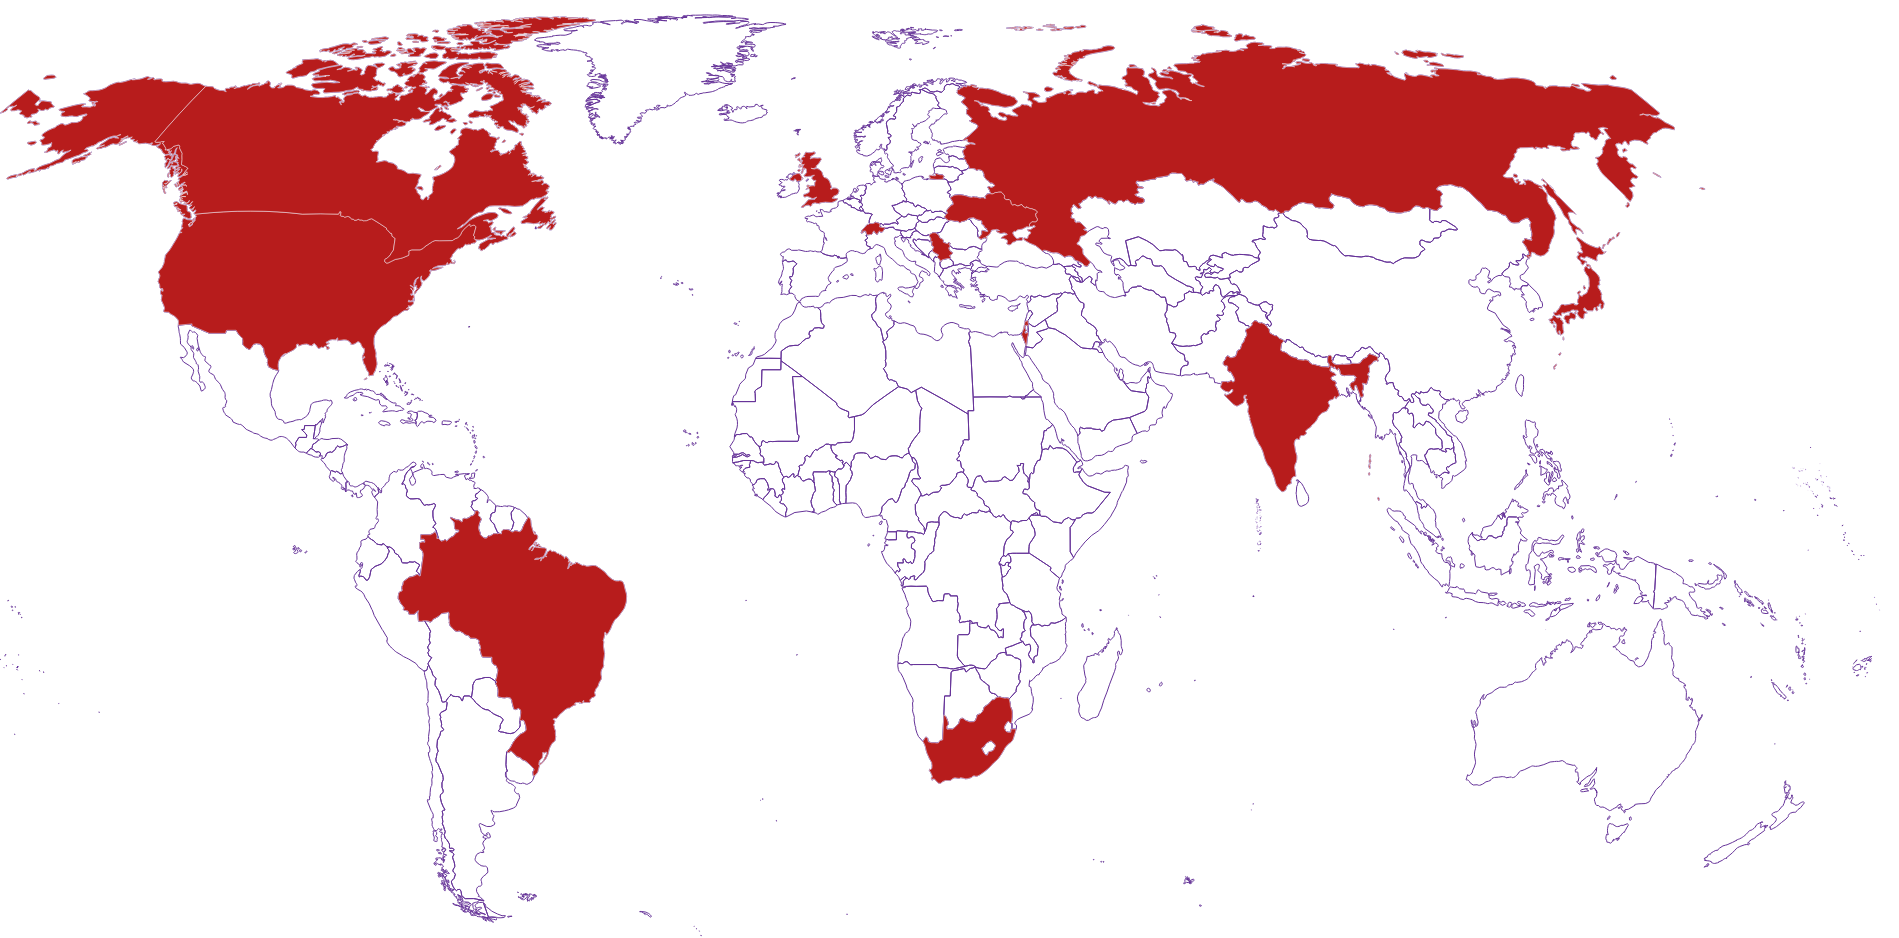
\includegraphics[width=\textwidth]{figures/images/figure_tracks_destinations_color_from_eea_no_scale.png}
        \caption{Destinations for traffic originating in the EEA.}
        \label{fig:destinations_from_eea}
    \end{subfigure}

    \vspace{0.5em}

    \begin{subfigure}{0.48\textwidth}
        \centering
        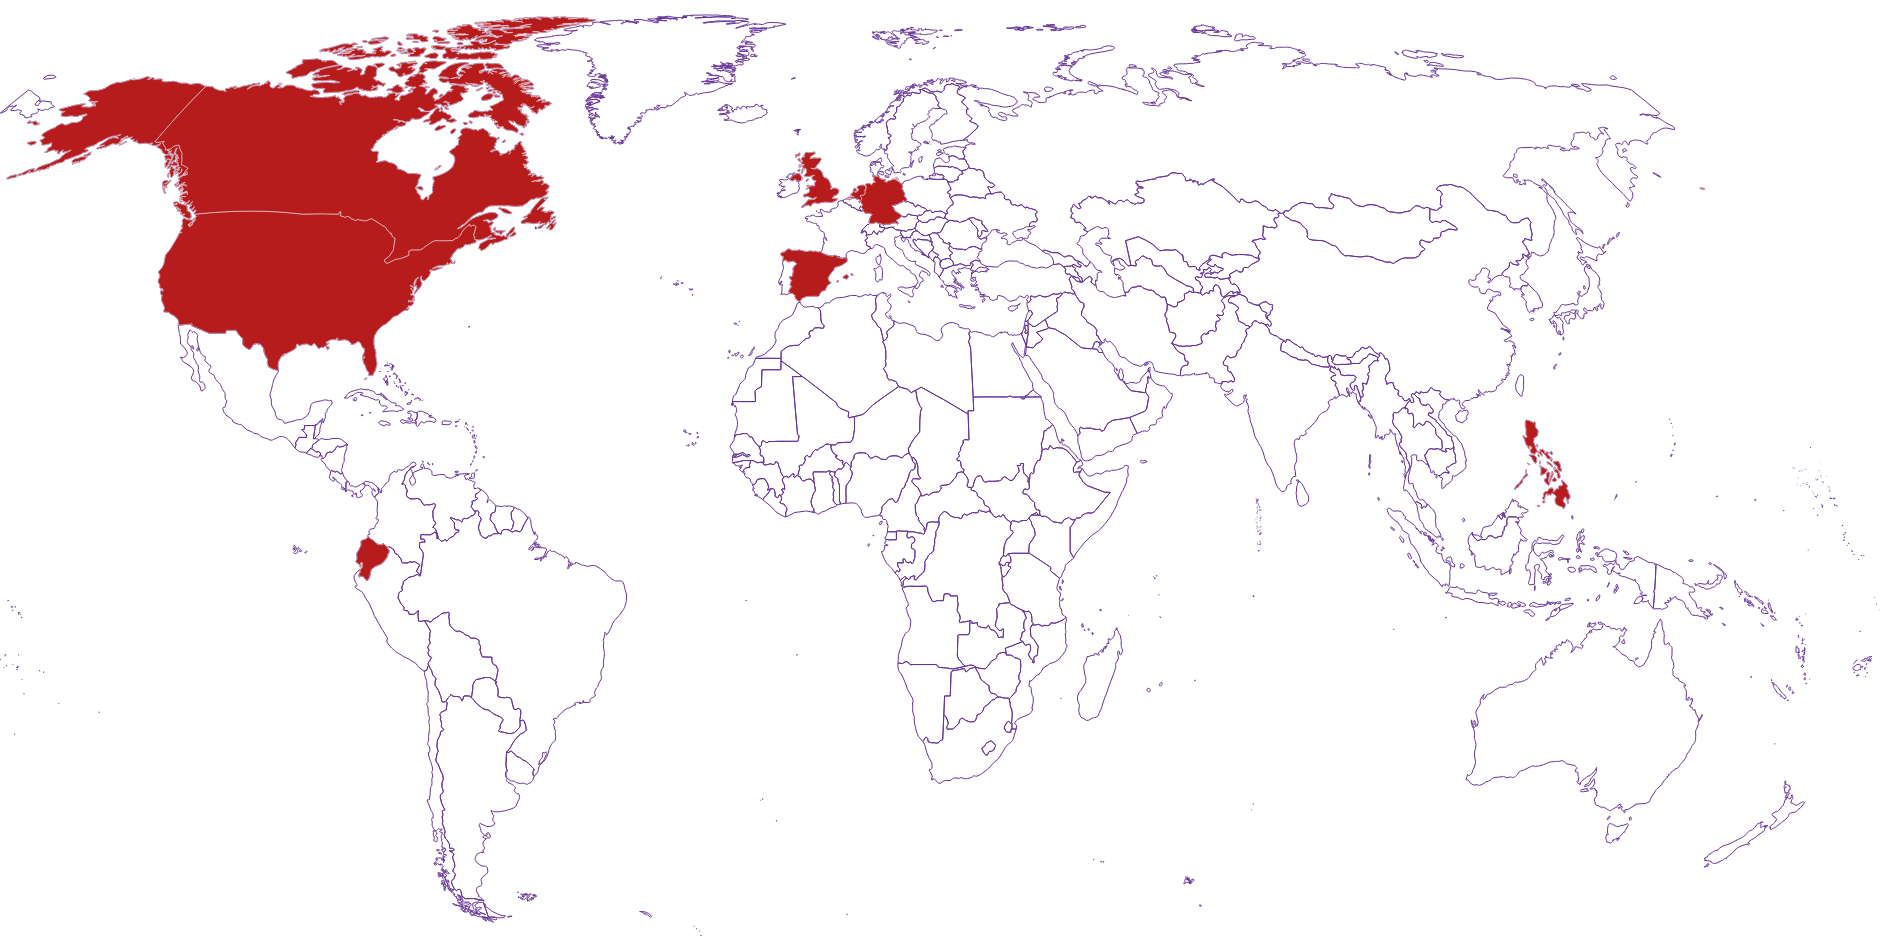
\includegraphics[width=\textwidth]{figures/images/figure_tracks_destinations_color_from_japan_no_scale.png}
        \caption{Destinations for traffic originating in Japan.}
        \label{fig:destinations_from_japan}
    \end{subfigure}
    \caption{Examples of geographic destinations observed during the global anycast measurement campaign.}
    \label{fig:visualization_global_hunter}
\end{figure}

The global measurements also revealed distinct regional routing patterns. Traffic originating in Latin America frequently terminated in the United States, reflecting the concentration of anycast infrastructure in North America. Conversely, communications originating in the United States were observed reaching destinations including Brazil, Japan, South Africa, the EEA, and Cuba. The measurements from the EEA also showed substantial external routing, with 34.88\% of communications terminating outside the region, including destinations such as Russia, India, and South Africa. In contrast, traffic originating in Japan, India, and South Korea exhibited stronger regional retention, while communications originating in African countries frequently terminated in Europe.

These observations generalise the findings obtained from the EEA-focused experiment. While the first experiment characterised cross-border anycast communications in the context of Android applications and personal-data \DIFdelbegin \DIFdel{transfers within }\DIFdelend \DIFaddbegin \DIFadd{communications originating in }\DIFaddend the EEA, the independent global campaign examined a broader set of anycast infrastructures and source locations worldwide. The EEA experiment demonstrated that personal-data communications generated by mobile applications may reach destinations outside the region, whereas the global campaign shows that similar cross-border routing behaviour occurs across multiple geographic contexts and is not specific to European networks or data protection requirements. The fact that 99.49\% of the analysed anycast IP addresses exhibited at least one cross-border routing event further indicates that the phenomenon is associated with the operational behaviour of the analysed anycast infrastructures rather than with a small subset of exceptional deployments.

The global experiment also provides a broader perspective on the relationship between geographic origin and destination. The observed routing patterns varied substantially across source regions: some regions exhibited frequent communication with infrastructure located in other continents, whereas others showed a stronger tendency to remain within their geographic region. Consequently, the geographic exposure associated with an anycast service cannot be inferred solely from the location of its infrastructure or from the location of the user. Instead, it depends on the interaction between the source network, the anycast deployment, and the routing policies governing the communication path.

Overall, the global measurements demonstrate that cross-border routing is a widespread characteristic of the analysed anycast infrastructures. The results therefore generalise the observations obtained from the EEA-specific Android experiment and show that the geographic uncertainty introduced by anycast is not limited to a particular jurisdiction, application ecosystem, or regulatory framework. This broader perspective motivates the need for mechanisms that allow service providers to impose explicit geographic constraints when the jurisdiction in which communications are processed is a relevant requirement.

% ============================================================
\section{Summary and Next Steps}
\label{sc:anycast_experiments_summary}
% ============================================================

This chapter has analysed the geographic implications of anycast communications from two complementary perspectives. First, the large-scale Android experiment \DIFdelbegin \DIFdel{demonstrated that}\DIFdelend \DIFaddbegin \DIFadd{showed that, in the analysed dataset, }\DIFaddend personal-data communications generated by applications and their embedded TPLs may \DIFdelbegin \DIFdel{reach destinations }\DIFdelend \DIFaddbegin \DIFadd{terminate in countries }\DIFaddend outside the EEA, \DIFdelbegin \DIFdel{while }\DIFdelend \DIFaddbegin \DIFadd{and }\DIFaddend the comparison with privacy policies revealed substantial discrepancies between \DIFdelbegin \DIFdel{observed destinations }\DIFdelend \DIFaddbegin \DIFadd{the destinations inferred }\DIFaddend and the jurisdictions disclosed to users. Second, the global measurement campaign extended the analysis beyond the Android ecosystem and the European context, showing that cross-border routing is \DIFdelbegin \DIFdel{widespread across operational anycast infrastructuresworldwide. }\DIFdelend \DIFaddbegin \DIFadd{common across the analysed anycast infrastructures. These observations reveal that personal data are frequently exposed to jurisdictions outside the EEA without users being informed. Some of the most frequent destinations, such as the United Kingdom and Switzerland, benefit from adequacy decisions, which mitigate the risk associated with the level of protection. However, an adequacy decision does not remove the obligation to inform data subjects about the intention to transfer their data and about the existence of that decision, so the discrepancies identified constitute relevant transparency gaps regardless of the destination. }\DIFaddend The results of the Android experiment have been published in the article \emph{Anycast and Third-Party Libraries: A Recipe for a Privacy Disaster?} \cite{Pascual2025AnycastDisaster} and the global measurement campaign is included in the manuscript currently under review presented in Chapter~\ref{ch:rcadns}.

Taken together, the results show that observing and measuring the geographic behaviour of anycast infrastructures is feasible, but that measurement alone does not provide service providers with deterministic control over the jurisdictions reached by their communications. This limitation motivates the next part of the thesis, which moves from analysing geographic exposure to investigating how geographic constraints can be explicitly enforced in anycast infrastructures. The following chapter therefore introduces the RCA-DNS architecture, which combines DNS-based service selection with geographically scoped anycast deployments to \DIFdelbegin \DIFdel{provide deterministic geographic control }\DIFdelend \DIFaddbegin \DIFadd{confine the processing of communications to selected regions }\DIFaddend while preserving the operational benefits of anycast.
 \newpage 
 \newpage \chapter{Geographic Regionalization of Anycast Services}
\label{ch:rcadns}

The previous chapters have shown that the geographic destination of an anycast communication is neither visible to users nor, in many cases, controlled by the organisations that operate the service. Chapter~\ref{ch:hunter} introduced Hunter, which makes it possible to infer the country in which an anycast communication terminates. Chapter~\ref{ch:experiments} then used Hunter to show that personal data sent by Android applications and their TPLs frequently reaches countries outside the EEA, often without being disclosed in privacy policies. The global campaign presented in Section~\ref{sc:anycast_experiments_global_anycast} confirmed that this behaviour is not specific to Europe: 58.36\% of the valid routing tracks terminated in a country different from the one in which they originated, and 99.49\% of the analysed anycast addresses exhibited at least one cross-border routing event.

These findings matter because, as discussed in Section~\ref{sc:background_privacy_regulations}, the lawfulness of data processing is increasingly tied to the place where it occurs. Data protection regulations restrict international transfers of personal data \cite{REGULATIONSRelevance, CourtII}, and the Data Act and the Data Governance Act extend comparable safeguards to non-personal data \cite{2022DataAct, 2022DataActb}. Whether framed in terms of data residency, data localisation, or data sovereignty (Section~\ref{sc:background_privacy_data_sovereignty}), these obligations share a common premise: the operator of a service must be able not only to know, but also to decide and later demonstrate, where communications are processed. Chapters~\ref{ch:hunter} and~\ref{ch:experiments} addressed the first part of this premise by making the destination of anycast communications observable. This chapter addresses the second.

Conventional anycast deployments do not offer this capability. Because every replica announces the same prefix and each AS independently selects among the resulting routes, the replica that serves a given user is the outcome of a distributed decision process in which geography and jurisdiction play no role. Operators can influence this process, for instance by adding or withdrawing replicas or by manipulating BGP announcements, but they cannot constrain it deterministically. As a consequence, an organisation that wants to guarantee that the communications of its European users are processed within the EEA currently faces a choice between keeping the operational advantages of anycast and obtaining geographic guarantees.

This chapter presents \textit{Region-Constrained Anycast over DNS} (RCA-DNS), an architecture that removes this trade-off. RCA-DNS exposes one DNS name per geographic region, maps each name to a different anycast address, and lets only the infrastructure located inside that region serve the address. The region is selected by the service before DNS resolution, according to its own policy, and the network is then responsible only for delivering traffic within the boundaries implied by that choice. This chapter addresses research question RQ4, which asks which architectural mechanisms can provide deterministic geographic control over anycast communications without significantly compromising scalability, performance, and resilience.

The remainder of the chapter is organised as follows. Section~\ref{sc:rcadns_related} reviews the existing approaches to geographic traffic control and explains why none of them satisfies the problem described above. Section~\ref{sc:rcadns_requirements} derives the requirements that guide the design. Section~\ref{sc:rcadns_architecture} describes the RCA-DNS architecture, its components, its communication workflow, and the different levels at which confinement can be enforced. Section~\ref{sc:rcadns_feasibility} analyses whether the architecture can be implemented on the platforms offered by major cloud and CDN providers. Section~\ref{sc:rcadns_evaluation} evaluates a prototype deployed on Google Cloud through an eight-day RIPE Atlas measurement campaign. Finally, Section~\ref{sc:rcadns_discussion} discusses the regulatory implications and the limitations of the proposal, and Section~\ref{sc:rcadns_summary} summarises the chapter.

% ============================================================
\section{Existing Approaches to Geographic Traffic Control}
\label{sc:rcadns_related}
% ============================================================

Several families of techniques can steer clients towards infrastructure located in a particular area. This section describes each of them and identifies why it does not, on its own, provide deterministic geographic control while preserving the benefits of anycast. Table~\ref{tab:rcadns_related_comparison} summarises the comparison.

\subsection{DNS-Based Request Routing}
\label{sc:rcadns_related_geodns}

DNS-based request routing, often referred to as GeoDNS, is the classical mechanism used by CDNs to map clients to nearby servers. When the authoritative DNS server of the CDN receives a query, it estimates the location of the client and returns the address of a server that is expected to perform well for that location. The estimation, however, is usually made from the address of the recursive resolver that issues the query rather than from the address of the client itself. Otto et al. showed that the widespread use of remote and public resolvers breaks the assumption that resolver and client are co-located, which leads to inaccurate mappings \cite{Otto2012ContentSolutions}. The EDNS Client Subnet extension (ECS) was standardised to mitigate this problem by letting resolvers forward a truncated client prefix to authoritative servers \cite{Contavalli2016ClientQueries}, and large CDNs have used it to deploy end-user mapping \cite{Chen2015End-UserDelivery}. ECS is nevertheless optional, is not supported by every resolver, and exposes part of the client address to additional parties, which conflicts with DNS privacy goals \cite{Bortzmeyer2015DNSConsiderations}.

Even when the client is located correctly, GeoDNS remains unsuitable for jurisdictional control for two reasons. First, the location is inferred from IP geolocation, whose accuracy has repeatedly been shown to be insufficient for compliance purposes \cite{Poese2011IPUnreliable, Cozar2022ReliabilityTransfers}; an error in the inference results in the client being mapped to the wrong region without the service being aware of it. Second, the mapping policy belongs to the CDN and is optimised for performance and load, not for the legal requirements of each customer. If the returned address is itself a global anycast address, BGP still decides which replica processes the request, and the geographic uncertainty documented in Chapter~\ref{ch:experiments} remains.

\subsection{Application-Level Filtering}
\label{sc:rcadns_related_filtering}

A second family of techniques enforces geographic restrictions at the application layer. The server inspects each incoming request, typically by geolocating the source IP address, and rejects, redirects, or treats it differently depending on its estimated origin. This approach is common for content licensing and for regulatory geo-blocking. As a mechanism for data residency, however, it acts too late: by the time the server evaluates the request, the request, including any personal data it carries, has already reached the replica selected by anycast routing and has been decrypted there. Filtering can therefore prevent a service from being delivered in a given location, but it cannot prevent data from being processed in an unintended jurisdiction. It also inherits the inaccuracy of IP geolocation discussed above.

\subsection{Independent Regional Deployments}
\label{sc:rcadns_related_regional}

The most widespread practical solution is to operate separate deployments for each region, each reachable through its own hostname and its own unicast addresses. Analytics and telemetry providers, which are among the TPLs analysed in Chapter~\ref{ch:experiments}, offer this option to customers subject to data residency requirements. Mixpanel, for example, provides EU and India residency programmes in which applications must configure the SDK to send data to a dedicated regional endpoint (e.g.\ \texttt{api-eu.mixpanel.com}) instead of the default one \cite{EUMixpanel}. This pattern demonstrates that selecting a regional hostname at the client is already accepted practice. However, when each regional hostname resolves to unicast infrastructure, the deployment loses the properties that motivate anycast: traffic within the region is not automatically distributed among replicas, failover relies on DNS updates whose propagation is bounded by record TTLs and resolver caching, and the absorption of volumetric attacks is concentrated on a few locations.

\subsection{Anycast Optimisation and Hybrid Schemes}
\label{sc:rcadns_related_optimisation}

Research on anycast has mostly targeted performance and operator control. Calder et al. and Koch et al. characterised the latency of large anycast services and found that a fraction of clients is systematically routed to distant replicas \cite{Calder2015AnalyzingCDN, Koch2021AnycastSystems}. Evang et al. defined metrics and BGP tuning techniques to improve client-to-site mapping and load distribution \cite{Evang2024AnycastTuning}, and Jia et al. proposed lightweight anycast services that combine DNS with explicit multicast routing \cite{Jia2019DeployingInternet}. Zhu et al. combined unicast, anycast, and modified BGP announcements to give operators finer control over the replica that serves each client; even in their fastest failover configuration, approximately 82\% of the requests were forwarded to replicas other than the intended one \cite{Zhu2022TheWorlds}. These techniques improve the average behaviour of anycast, but they continue to operate on routing preferences and therefore cannot guarantee where a specific communication terminates.

\subsection{Regional IP Anycast}
\label{sc:rcadns_related_regional_anycast}

The approach closest to RCA-DNS is regional IP anycast, studied by Zhou et al. in the deployments of the Edgio and Imperva CDNs \cite{Zhou2023RegionalPotentials}. These CDNs partition their replicas into regions, assign a distinct anycast prefix to each region, and use DNS together with IP geolocation to return to each client the prefix of its region. The authors found that both CDNs follow continent or country borders when defining regions and that regional anycast alleviates the pathology of global anycast in which BGP routes clients to distant replicas. They also observed that DNS occasionally returns the prefix of a remote region to a client, so that the client is served by an unintended regional network.

RCA-DNS reuses the central idea of regional anycast, namely one anycast address per region, but changes who selects the region and why. In regional IP anycast the region is chosen by the CDN, using geolocation, to optimise performance; the customer neither defines the regions nor decides which one applies to each communication. In RCA-DNS the region is a policy decision taken by the service itself before resolution, and the DNS mapping from name to address is static and independent of the location of the client or the resolver. As a result, the mapping errors observed by Zhou et al. cannot occur: if the service selects the EEA region, the name it resolves can only return the EEA address.

\subsection{Summary}
\label{sc:rcadns_related_summary}

Table~\ref{tab:rcadns_related_comparison} compares the approaches described above. GeoDNS and regional IP anycast rely on location inference and on a mapping policy controlled by the provider; application-level filtering acts after the data has already reached its destination; independent regional deployments sacrifice the benefits of anycast; and anycast optimisation techniques do not offer guarantees. Providers have also started to offer data localisation products that combine some of these elements. Because they are commercial implementations rather than general techniques, they are analysed separately in Section~\ref{sc:rcadns_feasibility}.

\begin{table}[ht]
    \centering
    \small
    \caption{Comparison of approaches to geographic traffic control. $\checkmark$: satisfied; $\sim$: partially satisfied; $\times$: not satisfied.}
    \label{tab:rcadns_related_comparison}
    \footnotesize
    \setlength{\tabcolsep}{3pt}
    \begin{tabularx}{\textwidth}{>{\raggedright\arraybackslash}X ccccc}
        \toprule
        \textbf{Approach} &
        \begin{tabular}[c]{@{}c@{}}\textbf{Deterministic}\\\textbf{confinement}\end{tabular} &
        \begin{tabular}[c]{@{}c@{}}\textbf{Anycast}\\\textbf{benefits}\end{tabular} &
        \begin{tabular}[c]{@{}c@{}}\textbf{Policy set}\\\textbf{by service}\end{tabular} &
        \begin{tabular}[c]{@{}c@{}}\textbf{No location}\\\textbf{inference}\end{tabular} &
        \begin{tabular}[c]{@{}c@{}}\textbf{No routing}\\\textbf{changes}\end{tabular} \\
        \midrule
        GeoDNS \cite{Otto2012ContentSolutions, Chen2015End-UserDelivery} & $\times$ & $\sim$ & $\times$ & $\times$ & $\checkmark$ \\
        \rowsep{6}
        Application-level filtering & $\times$ & $\checkmark$ & $\checkmark$ & $\times$ & $\checkmark$ \\
        \rowsep{6}
        Independent regional deployments \cite{EUMixpanel} & $\checkmark$ & $\times$ & $\checkmark$ & $\checkmark$ & $\checkmark$ \\
        \rowsep{6}
        Anycast optimisation and hybrid schemes \cite{Zhu2022TheWorlds, Evang2024AnycastTuning} & $\times$ & $\checkmark$ & $\sim$ & $\checkmark$ & $\times$ \\
        \rowsep{6}
        Regional IP anycast \cite{Zhou2023RegionalPotentials} & $\sim$ & $\checkmark$ & $\times$ & $\times$ & $\checkmark$ \\
        \midrule
        \textbf{RCA-DNS} (this chapter) & $\checkmark$ & $\checkmark$ & $\checkmark$ & $\checkmark$ & $\checkmark$ \\
        \bottomrule
    \end{tabularx}
\end{table}

% ============================================================
\section{Design Requirements}
\label{sc:rcadns_requirements}
% ============================================================

The analysis above shows that the challenge is not the use of anycast itself, but the absence of a mechanism that allows operators to bound the set of replicas that routing is allowed to choose from. The following requirements guide the design of RCA-DNS. They are referenced throughout the chapter and revisited in Section~\ref{sc:rcadns_discussion}.

\begin{itemize}
    \item \textbf{R1 -- Deterministic confinement.} Once a region has been selected for a communication, the communication must be processed only by infrastructure located in that region, independently of routing dynamics, resolver location, or geolocation errors.

    \item \textbf{R2 -- Compatibility with existing infrastructures.} The solution must rely on standard Internet protocols and require no modification of routing protocols, DNS, or client operating systems.

    \item \textbf{R3 -- Incremental deployability.} A service provider must be able to adopt the mechanism unilaterally, without coordination with third-party network operators, and service by service.

    \item \textbf{R4 -- Preservation of anycast benefits.} Within each region, the solution must retain the load distribution, resilience, automatic failover, and low latency associated with anycast.

    \item \textbf{R5 -- Operational simplicity.} The mechanism must be manageable with the configuration tools and practices that operators already use.

    \item \textbf{R6 -- Policy flexibility.} Regions must be definable according to legal, contractual, or business criteria (for instance the EEA, a single country, or the EEA together with countries covered by adequacy decisions), and the rule that assigns communications to regions must remain under the control of the service.
\end{itemize}

% ============================================================
\section{RCA-DNS Architecture}
\label{sc:rcadns_architecture}
% ============================================================

\subsection{Architecture Overview}
\label{sc:rcadns_overview}

The central idea of RCA-DNS is to separate two decisions that conventional anycast couples implicitly: \textit{which region should process a communication} and \textit{which replica within that region should process it}. In a conventional deployment both decisions are delegated to BGP. In RCA-DNS the first decision is a policy decision taken by the service before DNS resolution, while the second remains a routing decision taken by BGP, but only among replicas that already satisfy the policy. The architecture and workflow figures in this chapter use a common set of illustrative addresses from the documentation ranges, so that the same regional address (e.g.\ \texttt{203.0.113.20} for the EEA-Extended region) can be followed across them. The DNS zone in Figure~\ref{fig:rcadns_zone}, in contrast, shows the real addresses used in the prototype.

Figure~\ref{fig:rcadns_architecture} illustrates the resulting architecture. It distinguishes a \textit{policy plane}, in which the region is selected and translated into a DNS name, and a \textit{data plane}, in which traffic is delivered through standard anycast routing. The architecture comprises four elements:

\begin{itemize}
    \item \textbf{Regional anycast deployments.} For each region, the provider operates a set of replicas located exclusively within the region. All replicas of a region serve a dedicated anycast address that no replica outside the region serves.

    \item \textbf{Regional DNS records.} The authoritative zone of the service contains one name per region (e.g.\ \texttt{eea-extended.anycastprivacy.org}), each resolving to the anycast address of the corresponding regional deployment. Optionally, a \texttt{global} name resolves to an address served by all replicas, for communications that are not subject to geographic restrictions.

    \item \textbf{Region selection policy.} A component on the service side, typically in the client application or in its configuration, decides which region applies to each communication and therefore which name is used.

    \item \textbf{Standard Internet routing.} Once the name has been resolved, packets follow the routes selected by BGP towards one of the replicas that announce the regional address, exactly as in any other anycast service.
\end{itemize}

\begin{figure}[ht]
    \centering
    \resizebox{\textwidth}{!}{\begin{tikzpicture}[
    >=Latex,
    font=\small
]

% ------------------------------------------------------------
% Policy plane: client application and authoritative DNS
% ------------------------------------------------------------

\node[endpoint, minimum width=52mm, minimum height=27mm, anchor=north] (client) at (27mm,0) {};
\node[font=\footnotesize\bfseries, anchor=north, inner sep=2mm] at (client.north) {Client application};
\node[policy, anchor=south] (policy) at ($(client.south)+(0,3mm)$)
    {Region selection policy\\\scriptsize(user, contract, geolocation, \ldots)};

\node[dnszone, anchor=north east] (zone) at (164mm,0) {
    \textbf{Authoritative zone} \texttt{anycastprivacy.org}\\[0.5mm]
    \begin{tabular}{@{}l@{\hspace{2mm}}c@{\hspace{2mm}}l@{}}
        \texttt{global}       & $\rightarrow$ & \texttt{203.0.113.10} \\
        \texttt{eea-extended} & $\rightarrow$ & \texttt{203.0.113.20} \\
        \texttt{us}           & $\rightarrow$ & \texttt{203.0.113.30} \\
        \texttt{asia}         & $\rightarrow$ & \texttt{203.0.113.40} \\
    \end{tabular}
};

\coordinate (qa) at ($(client.east)+(0,5mm)$);
\coordinate (qb) at ($(client.east)+(0,-5mm)$);
\draw[dnsflow] (qa) -- node[above, font=\scriptsize, align=center]
    {DNS query\\\texttt{eea-extended.anycastprivacy.org}} (qa -| zone.west);
\draw[dnsflow, dashed] (qb -| zone.west) -- node[below, font=\scriptsize, align=center]
    {DNS answer\\\texttt{A 203.0.113.20}} (qb);

\node[steplabel] at ($(policy.west)+(-5mm,0)$) {1};
\node[steplabel] at ($(qa)!0.5!(qa -| zone.west)+(0,13mm)$) {2};

% ------------------------------------------------------------
% Data plane: regional anycast deployments
% ------------------------------------------------------------

% EEA-Extended
\node[anycastip, minimum width=30mm] (ipeea) at (27mm,-58mm)
    {Anycast IP\\\texttt{203.0.113.20}};
\node[replica, minimum width=21mm, font=\footnotesize] (eea1) at (15mm,-80mm) {Madrid};
\node[replica, minimum width=21mm, font=\footnotesize] (eea2) at (39mm,-80mm) {Frankfurt};
\node[replica, minimum width=21mm, font=\footnotesize] (eea3) at (27mm,-92mm) {Paris};
\begin{scope}[on background layer]
    \node[regionbox, fit=(ipeea)(eea1)(eea2)(eea3), inner ysep=7mm] (regeea) {};
\end{scope}
\node[regionlabel, anchor=south west] at (regeea.south west) {EEA-Extended region};

% US
\node[anycastip, minimum width=30mm] (ipus) at (84mm,-58mm)
    {Anycast IP\\\texttt{203.0.113.30}};
\node[replica, minimum width=21mm, font=\footnotesize] (us1) at (72mm,-80mm) {Iowa};
\node[replica, minimum width=21mm, font=\footnotesize] (us2) at (96mm,-80mm) {Virginia};
\node[replica, minimum width=21mm, font=\footnotesize] (us3) at (84mm,-92mm) {Oregon};
\begin{scope}[on background layer]
    \node[regionbox, fit=(ipus)(us1)(us2)(us3), inner ysep=7mm] (regus) {};
\end{scope}
\node[regionlabel, anchor=south west] at (regus.south west) {US region};

% Asia
\node[anycastip, minimum width=30mm] (ipasia) at (141mm,-58mm)
    {Anycast IP\\\texttt{203.0.113.40}};
\node[replica, minimum width=21mm, font=\footnotesize] (as1) at (129mm,-80mm) {Tokyo};
\node[replica, minimum width=21mm, font=\footnotesize] (as2) at (153mm,-80mm) {Singapore};
\node[replica, minimum width=21mm, font=\footnotesize] (as3) at (141mm,-92mm) {Mumbai};
\begin{scope}[on background layer]
    \node[regionbox, fit=(ipasia)(as1)(as2)(as3), inner ysep=7mm] (regasia) {};
\end{scope}
\node[regionlabel, anchor=south west] at (regasia.south west) {Asia region};

% Anycast announcements inside each region
\foreach \ip/\a/\b/\c in {ipeea/eea1/eea2/eea3, ipus/us1/us2/us3, ipasia/as1/as2/as3} {
    \draw[replicaLink] (\ip.south) -- (\a.north);
    \draw[replicaLink] (\ip.south) -- (\b.north);
    \draw[replicaLink] (\ip.south) -- (\c.north);
}

% Global deployment (all replicas)
\begin{scope}[on background layer]
    \node[draw=violet!60, dotted, line width=1pt, rounded corners=8pt,
          fit=(regeea)(regus)(regasia), inner sep=3mm] (global) {};
\end{scope}
\node[font=\footnotesize\itshape, text=violet!70!black, anchor=north east, inner sep=1.5mm]
    at (global.south east) {\texttt{global.anycastprivacy.org} (\texttt{203.0.113.10}) is announced by every replica};

% Traffic from the client to the selected regional anycast address
\draw[bgppath] (client.south) -- (ipeea.north);
\node[font=\scriptsize, align=left, anchor=west, text=blue!70!black] at ($(client.south)!0.45!(ipeea.north)+(3mm,0)$)
    {HTTPS to \texttt{203.0.113.20} over standard BGP anycast routing:\\
     only instances inside the EEA-Extended region announce this address};
\node[steplabel] at ($(client.south)!0.45!(ipeea.north)+(-4mm,0)$) {3};

\end{tikzpicture}
}
    \caption{RCA-DNS architecture. (1) The client application selects a region according to its policy; (2) it resolves the name associated with that region, which always returns the same regional anycast address; (3) packets follow the routes selected by BGP towards one of the replicas that announce that address, all of which are located inside the selected region.}
    \label{fig:rcadns_architecture}
\end{figure}

Because geographic constraints are enforced by the choice of name, traffic engineering, load balancing, and failover continue to be handled within each region by the usual anycast mechanisms. RCA-DNS does not require changes to routing protocols, to DNS, or to the operating system of the client (R2), and each service can adopt it independently (R3).

\subsection{Regional DNS Records}
\label{sc:rcadns_records}

Figure~\ref{fig:rcadns_zone} shows the zone that implements RCA-DNS for the prototype evaluated in Section~\ref{sc:rcadns_evaluation}. Each record corresponds to one of the regions defined on Google Cloud and resolves to the anycast address of a deployment that only includes the locations of that region. The record \texttt{global} resolves to an address served by every location and reproduces a conventional anycast service.

\begin{figure}[ht]
    \centering
\begin{Verbatim}[fontsize=\footnotesize, frame=single, framesep=3mm, rulecolor=\color{black!55}]
$ORIGIN anycastprivacy.org.
; ---------------------------------------------------------------
; RCA-DNS: one name and one anycast address per region
; ---------------------------------------------------------------
global          IN  A   136.69.74.5    ; all 39 locations
eea-extended    IN  A   8.232.14.99    ; 13 locations (EEA, UK, CH)
us              IN  A   136.68.198.50  ;  9 locations
northamerica    IN  A   8.232.205.19   ;  3 locations (CA, MX)
southamerica    IN  A   136.69.55.215  ;  2 locations (BR, CL)
asia            IN  A   34.50.157.186  ;  9 locations
australia       IN  A   136.68.142.0   ;  2 locations
africa          IN  A   136.69.107.84  ;  1 location  (ZA)
\end{Verbatim}
    \caption{Authoritative zone implementing RCA-DNS in the prototype evaluated in this chapter. Each name resolves to a different anycast address, served only by the Google Cloud locations of the corresponding region. Unlike in the other figures, the addresses shown are the real ones assigned by Google Cloud to the prototype during the measurement campaign (July 2026); they may have been reassigned since the deployment was removed.}
    \label{fig:rcadns_zone}
\end{figure}

Three properties of these records are relevant for the design.

\paragraph{Location-independent mapping.} Unlike GeoDNS, the answer to each query does not depend on who asks. Any resolver, public or private, located anywhere in the world, returns the same address for \texttt{eea-extended.anycastprivacy.org}. The correctness of RCA-DNS is therefore unaffected by the use of public resolvers, by the absence of ECS, or by DNS over encrypted transports, which are precisely the factors that degrade GeoDNS \cite{Otto2012ContentSolutions, Contavalli2016ClientQueries}. This property is what makes the confinement deterministic (R1) once the region has been chosen.

\paragraph{Stable records and caching.} Because the mapping between names and addresses changes only when the provider reorganises its deployment, records can use long TTLs and benefit fully from resolver caching. Changes of region do not require changing any record: the client simply uses a different name. Changes in the composition of a region, such as adding a new location, are absorbed by the anycast deployment and do not alter the address, so they do not require DNS updates either.

\paragraph{Address requirements.} RCA-DNS requires one anycast address per region and service. On managed platforms, such as the one used in the prototype, each address is allocated by the provider together with the corresponding load balancer. Operators that announce their own prefixes must take into account that inter-domain routing filters prefixes longer than a /24 in IPv4 (or a /48 in IPv6), so each region requires its own routable prefix. This is manageable in practice: IPv6 provides ample address space, and a single regional IPv4 address can be shared among many services, which are then demultiplexed using the Server Name Indication (SNI) or the HTTP \texttt{Host} header, as infrastructure providers commonly do.

\subsection{Region Determination}
\label{sc:rcadns_region_determination}

Determining which region should apply to a communication is outside the scope of RCA-DNS and of this thesis. This decision belongs entirely to the service, and the architecture only requires that it be taken before DNS resolution. This separation is intentional: the appropriate criterion depends on the legal basis of the processing and on the application domain, and the routing mechanism should not have to change when the criterion does (R6). RCA-DNS therefore guarantees that the selected region is respected, but makes no assumption about how it is selected. For illustrative purposes only, Table~\ref{tab:rcadns_region_mechanisms} summarises some of the mechanisms that a service could use, which are briefly described below.

\begin{itemize}
    \item \textbf{Explicit user declaration.} The user states the country or region of residence, for example during registration. This is simple and transparent, but relies on the honesty and accuracy of the user. It is appropriate when the applicable jurisdiction is linked to residence rather than to the momentary location of the device.

    \item \textbf{Account or contractual attributes.} The region is derived from information that the service already holds, such as the billing country, the legal entity that signed the contract, or the tenant region in a business-to-business deployment. This is the most robust mechanism when obligations derive from a contract, as is common for enterprise customers that require data residency.

    \item \textbf{Enterprise policy.} In managed environments, the region can be imposed by the organisation through device management or application configuration, so that all communications generated by corporate devices use the region required by internal compliance policies.

    \item \textbf{Coarse IP geolocation.} The service geolocates the client address, typically at login or when downloading its configuration. It requires no user interaction, but it inherits the inaccuracies of geolocation databases \cite{Poese2011IPUnreliable, Cozar2022ReliabilityTransfers} and can be circumvented by VPNs. It is therefore best used as a default that other signals can override.

    \item \textbf{Device location.} The application uses the location services of the operating system. It is the most precise signal of where the device is, but requires a permission and processes additional personal data, which conflicts with the data minimisation principle unless the location is already needed by the service.

    \item \textbf{Fixed regulatory scope.} When a service is only offered in a single jurisdiction, for instance a public health application, the region can simply be fixed in the application.
\end{itemize}

\begin{table}[ht]
    \centering
    \small
    \caption{Examples of mechanisms that a service could use to determine the region of a communication before DNS resolution.}
    \label{tab:rcadns_region_mechanisms}
    \begin{tabularx}{\textwidth}{>{\raggedright\arraybackslash}p{3.3cm} >{\raggedright\arraybackslash}X >{\raggedright\arraybackslash}p{2.0cm} >{\raggedright\arraybackslash}p{2.3cm}}
        \toprule
        \textbf{Mechanism} & \textbf{Signal} & \textbf{Robustness} & \textbf{Additional personal data} \\
        \midrule
        User declaration & Country of residence stated by the user & Medium & Minimal \\
        \rowsep{4}
        Account / contract & Billing country, contracting entity, tenant region & High & None \\
        \rowsep{4}
        Enterprise policy & Configuration imposed on managed devices & High & None \\
        \rowsep{4}
        Coarse IP geolocation & Client address at login or configuration time & Low--medium & Low \\
        \rowsep{4}
        Device location & Operating system location services & High & High \\
        \rowsep{4}
        Fixed regulatory scope & Hard-coded region & High & None \\
        \bottomrule
    \end{tabularx}
\end{table}

The decision can be implemented directly in the code of the application or, more flexibly, delivered as part of its remote configuration, so that the service can change the region assigned to a user without publishing a new version. The same applies to TPLs: as the Mixpanel example in Section~\ref{sc:rcadns_related_regional} shows, SDKs can expose the endpoint as a configuration parameter, which allows the developer of the host application to apply its own policy to the communications generated by embedded libraries. This is particularly relevant given that, as shown in Chapter~\ref{ch:experiments}, a large share of the cross-border personal-data communications observed in Android applications originate from TPLs.

\subsection{Communication Workflow}
\label{sc:rcadns_workflow}

Figure~\ref{fig:rcadns_sequence} details the messages exchanged when a client application communicates with a service that implements RCA-DNS.

\begin{figure}[ht]
    \centering
    \resizebox{\textwidth}{!}{\begin{tikzpicture}[
    >=Latex,
    font=\small
]

% ------------------------------------------------------------
% Participants
% ------------------------------------------------------------

\node[lifelinehead, fill=yellow!15] (app) at (0,0)
    {Client application\\\scriptsize(region policy)};
\node[lifelinehead] (res) at (44mm,0)
    {Recursive\\resolver};
\node[lifelinehead, fill=orange!8] (auth) at (88mm,0)
    {Authoritative DNS\\\scriptsize\texttt{anycastprivacy.org}};
\node[lifelinehead, fill=green!8] (rep) at (138mm,0)
    {Regional anycast service\\\scriptsize(EEA-Extended instances)};

\def\ybottom{-128mm}
\foreach \p in {app,res,auth,rep} {
    \draw[lifeline] (\p.south) -- (\p.south |- 0,\ybottom);
}

% ------------------------------------------------------------
% (1) Region selection
% ------------------------------------------------------------

\draw[msg] ($(app.south)+(0,-8mm)$) -- ++(7mm,0) -- ++(0,-5mm) -- ++(-7mm,0);
\node[msglabel, anchor=west, align=left] at ($(app.south)+(8.5mm,-10.5mm)$)
    {\textbf{1} \;select region $R$ = \texttt{eea-extended}\\
     \phantom{\textbf{1}} \;$\Rightarrow$ name \texttt{eea-extended.anycastprivacy.org}};

% ------------------------------------------------------------
% (2)-(5) DNS resolution
% ------------------------------------------------------------

\draw[msg] (app.south |- 0,-28mm) -- node[msglabel, above=0.5mm]
    {\textbf{2}\; \texttt{A? eea-extended.anycastprivacy.org}} (res.south |- 0,-28mm);

% optional fragment: cache miss
\draw[black!55, rounded corners=1pt] (38mm,-33mm) rectangle (96mm,-55mm);
\node[draw=black!55, fill=gray!10, font=\scriptsize\bfseries, anchor=north west, inner sep=1.2pt]
    at (38mm,-33mm) {opt};
\node[font=\scriptsize\itshape, anchor=north east, fill=white, inner sep=1pt] at (95.5mm,-33.5mm) {[cache miss]};

\draw[msg] (res.south |- 0,-41mm) -- node[msglabel, above=0.5mm]
    {\textbf{3}\; \texttt{A? eea-extended\ldots}} (auth.south |- 0,-41mm);
\draw[reply] (auth.south |- 0,-50mm) -- node[msglabel, above=0.5mm]
    {\textbf{4}\; \texttt{A 203.0.113.20}, TTL} (res.south |- 0,-50mm);

\draw[reply] (res.south |- 0,-62mm) -- node[msglabel, above=0.5mm]
    {\textbf{5}\; \texttt{A 203.0.113.20}} (app.south |- 0,-62mm);

% ------------------------------------------------------------
% (6)-(8) Data exchange over anycast
% ------------------------------------------------------------

\draw[encrypted] (app.south |- 0,-76mm) -- node[msglabel, above=0.5mm, pos=0.5]
    {\textbf{6}\; TCP + TLS handshake to \texttt{203.0.113.20} (SNI \texttt{eea-extended\ldots})} (rep.south |- 0,-76mm);
\node[font=\scriptsize\itshape, align=center, text=blue!70!black, fill=white, inner sep=1pt]
    at ($(rep.south |- 0,-76mm)+(-24mm,-4.5mm)$)
    {BGP routes lead the packets to the closest in-region instance};

\draw[encrypted] (app.south |- 0,-90mm) -- node[msglabel, above=0.5mm]
    {\textbf{7}\; HTTPS request (personal data)} (rep.south |- 0,-90mm);
\draw[reply, draw=green!50!black, line width=1.1pt] (rep.south |- 0,-100mm) -- node[msglabel, above=0.5mm]
    {\textbf{8}\; HTTPS response} (app.south |- 0,-100mm);

% ------------------------------------------------------------
% Policy re-evaluation
% ------------------------------------------------------------

\draw[black!55, rounded corners=1pt] (-14mm,-106mm) rectangle (158mm,-124mm);
\node[draw=black!55, fill=gray!10, font=\scriptsize\bfseries, anchor=north west, inner sep=1.2pt]
    at (-14mm,-106mm) {loop};
\node[font=\scriptsize, align=center, fill=white, inner sep=1.5pt] at (72mm,-115.5mm)
    {[policy change (e.g.\ new contract, user relocation) or TTL expiry]\\
     repeat from \textbf{1}: a different region yields a different name and, therefore, a different anycast address};

\end{tikzpicture}
}
    \caption{Sequence diagram of a communication under RCA-DNS. Steps 3 and 4 only occur when the record is not cached by the resolver. The answer obtained in step 5 is the same regardless of the location of the client or the resolver.}
    \label{fig:rcadns_sequence}
\end{figure}

\begin{enumerate}
    \item \textbf{Region selection.} Before the communication starts, the application evaluates its region selection policy and obtains a region $R$, in the example \texttt{eea-extended}. The region determines the name that will be used, \texttt{eea-extended.anycastprivacy.org}.

    \item \textbf{Query.} The application, through the stub resolver of the operating system, asks its recursive resolver for the address associated with that name.

    \item[3--4.] \textbf{Authoritative resolution.} If the record is not cached, the recursive resolver queries the authoritative server of \texttt{anycastprivacy.org}, which returns the regional anycast address together with its TTL.

    \setcounter{enumi}{4}
    \item \textbf{Answer.} The resolver returns the address \texttt{203.0.113.20} to the application.

    \item \textbf{Connection establishment.} The application opens a TCP connection and performs a TLS handshake with \texttt{203.0.113.20}, indicating the regional name in the SNI extension. Since only replicas located in the EEA-Extended region announce this address, the routes selected by BGP can only lead to one of them, normally the topologically closest.

    \item[7--8.] \textbf{Data exchange.} The application sends the HTTPS request, which may contain personal data, and receives the response from the same in-region replica.
\end{enumerate}

The selected region remains valid until the policy produces a different result, for example because the contractual situation of the user changes, or until the application re-evaluates it. In that case the workflow starts again from step 1 with a different name and, consequently, a different anycast address. Since names are static, there is no risk of a stale cache entry pointing to a replica in the wrong region.

\subsection{Enforcement Levels and the Role of Encryption}
\label{sc:rcadns_enforcement}

The description above assumes that the regional address is served only from inside the region. In practice, the point at which this guarantee is enforced depends on how the provider implements anycast, and three levels can be distinguished. Figure~\ref{fig:rcadns_enforcement_levels} illustrates them for a user located in the protected region whose traffic would, under BGP, enter the provider's network at a point of presence (PoP) outside the region, a situation that Chapter~\ref{ch:experiments} showed to be common.

\begin{figure}[ht]
    \centering
    \resizebox{\textwidth}{!}{\begin{tikzpicture}[
    >=Latex,
    font=\small
]

% ------------------------------------------------------------
% Background columns
% ------------------------------------------------------------

\fill[red!4]   (31mm,6mm) rectangle (87mm,-86mm);
\fill[green!5] (89mm,6mm) rectangle (162mm,-86mm);
\node[header] at (59mm,2mm)  {Outside the protected region};
\node[header] at (125mm,2mm) {Inside the protected region};
\node[header] at (14mm,2mm)  {Client};

% ------------------------------------------------------------
% Row (a): backend confinement
% ------------------------------------------------------------

\node[font=\footnotesize\bfseries, anchor=west] at (-6mm,-8mm)
    {(a) Backend confinement (provider-mediated)};
\node[endpoint, minimum width=22mm, font=\footnotesize] (ca) at (14mm,-20mm) {User\\in the region};
\node[ixp, minimum width=30mm, minimum height=10mm, font=\footnotesize] (pa) at (59mm,-20mm)
    {Edge PoP\\TLS terminated};
\node[replica, minimum width=30mm, font=\footnotesize] (ba) at (138mm,-20mm) {Regional backend\\(processing)};
\draw[encrypted] (ca) -- node[above, font=\scriptsize] {TLS} (pa);
\draw[cleartext] (pa) -- node[above, font=\scriptsize, align=center] {decrypted at the edge,\\re-encrypted to backend} (ba);

% ------------------------------------------------------------
% Row (b): in-region termination
% ------------------------------------------------------------

\node[font=\footnotesize\bfseries, anchor=west] at (-6mm,-36mm)
    {(b) In-region termination};
\node[endpoint, minimum width=22mm, font=\footnotesize] (cb) at (14mm,-48mm) {User\\in the region};
\node[ixp, minimum width=30mm, minimum height=10mm, font=\footnotesize] (pb) at (59mm,-48mm)
    {Edge PoP\\forwards ciphertext};
\node[ixp, minimum width=24mm, minimum height=10mm, font=\footnotesize, fill=green!12] (tb) at (106mm,-48mm)
    {In-region\\TLS end};
\node[replica, minimum width=30mm, font=\footnotesize] (bb) at (143mm,-48mm) {Regional backend\\(processing)};
\draw[encrypted] (cb) -- node[above, font=\scriptsize] {TLS} (pb);
\draw[encrypted] (pb) -- node[above, font=\scriptsize] {TLS} (tb);
\draw[link, ->] (tb) -- (bb);

% ------------------------------------------------------------
% Row (c): announcement confinement
% ------------------------------------------------------------

\node[font=\footnotesize\bfseries, anchor=west] at (-6mm,-64mm)
    {(c) Announcement confinement};
\node[endpoint, minimum width=22mm, font=\footnotesize] (cc) at (14mm,-76mm) {User\\in the region};
\node[ixp, minimum width=30mm, minimum height=10mm, font=\footnotesize, fill=gray!8, text=black!50, dashed] (pc) at (59mm,-76mm)
    {Edge PoP\\(prefix not announced)};
\node[ixp, minimum width=24mm, minimum height=10mm, font=\footnotesize, fill=green!12] (ic) at (106mm,-76mm)
    {In-region\\ingress + TLS end};
\node[replica, minimum width=30mm, font=\footnotesize] (bc) at (143mm,-76mm) {Regional backend\\(processing)};
\draw[encrypted] (cc.south east) to[out=-15,in=-165] node[below, font=\scriptsize] {TLS (transit may cross other countries)} (ic.south west);
\draw[link, ->] (ic) -- (bc);

% ------------------------------------------------------------
% Legend
% ------------------------------------------------------------

\draw[encrypted] (0mm,-94mm) -- ++(9mm,0);
\node[font=\scriptsize, anchor=west] at (10mm,-94mm) {payload only readable inside the protected region};
\draw[cleartext] (82mm,-94mm) -- ++(9mm,0);
\node[font=\scriptsize, anchor=west] at (92mm,-94mm) {payload decrypted outside the protected region};

\end{tikzpicture}
}
    \caption{Levels at which an RCA-DNS deployment can enforce geographic confinement, for a user located in the protected region whose traffic would enter the provider's network outside it.}
    \label{fig:rcadns_enforcement_levels}
\end{figure}

\begin{itemize}
    \item \textbf{(a) Backend confinement.} The regional address is announced from the provider's global edge, and the provider forwards requests only to backends located in the region, so the application logic and any associated storage are confined to the region. However, a layer-7 load balancer must read each request in order to route it, so the edge proxy that receives the connection necessarily acts as the TLS endpoint: it holds the private key of the certificate, negotiates the session keys with the client, and decrypts the request before opening a separate connection towards the regional backend. The content of every request is therefore available in clear at the point of presence where it entered the provider's network, which may be outside the region. This is the behaviour of global layer-7 load balancers. 

    \item \textbf{(b) In-region termination.} The address is still announced globally, but the elements outside the region forward the encrypted stream without decrypting it, either by relaying packets or by proxying the transport connection, and the TLS endpoint is located only inside the region. Since the session keys are negotiated through an ephemeral key exchange between the client and this endpoint, and the elements outside the region hold neither the private key nor the session keys, they only handle ciphertext. They can nevertheless observe metadata, such as the client IP address, the size and timing of the messages, and the \DIFdelbegin \DIFdel{server name indicated }\DIFdelend \DIFaddbegin \DIFadd{SNI included }\DIFaddend in the TLS handshake. The in-region TLS endpoint may be the application server itself or a component of the provider located in the region, so this level determines where content can be decrypted, not whether the provider can access it.

    \item \textbf{(c) Announcement confinement.} The regional prefix is originated only by replicas inside the region. Although the prefix remains reachable from anywhere, the routes selected by BGP can only lead to those replicas, so the first element of the provider that receives the packets, and the TLS endpoint, are necessarily located inside the region. Outside the region, packets only traverse third-party transit networks, which handle ciphertext and the same metadata as in level (b). This is the strictest form of confinement and corresponds to the original definition of regional anycast. Route leaks or hijacks could still divert traffic to other networks, a risk that origin validation through RPKI mitigates and that, in any case, would only expose ciphertext.
\end{itemize}

Table~\ref{tab:rcadns_enforcement_comparison} summarises the differences between the three levels and the limits of each of them

\begin{table}[ht]
    \centering
    \small
    \caption{Comparison of the enforcement levels of RCA-DNS from the point of view of a communication protected by TLS. ``Outside the region'' refers to the elements located outside the protected region.}
    \label{tab:rcadns_enforcement_comparison}
    \begin{tabularx}{\textwidth}{>{\raggedright\arraybackslash}p{3.4cm} >{\raggedright\arraybackslash}X >{\raggedright\arraybackslash}X >{\raggedright\arraybackslash}X}
        \toprule
        & \textbf{(a) Backend confinement} & \textbf{(b) In-region termination} & \textbf{(c) Announcement confinement} \\
        \midrule
        TLS endpoint (key negotiation and decryption) & Provider's edge, possibly outside the region & Inside the region & Inside the region \\
        \rowsep{4}
        Visible to the provider outside the region & Full content and metadata & Metadata only & Nothing (traffic does not reach the provider outside the region) \\
        \rowsep{4}
        Visible to transit networks & Ciphertext and metadata & Ciphertext and metadata & Ciphertext and metadata \\
        \rowsep{4}
        Provider access to content & Yes, possibly outside the region & Yes, only inside the region & Yes, only inside the region \\
        \rowsep{4}
        Example implementations (Section~\ref{sc:rcadns_feasibility}) & Global layer-7 load balancers (e.g.\ Google Cloud) & AWS Global Accelerator, Azure cross-region Load Balancer, Cloudflare Regional Services & Regional IP anycast, self-operated AS or BYOIP \\
        \bottomrule
    \end{tabularx}
\end{table}

In all three levels, the network path between the client and the provider is determined by inter-domain routing and may cross third countries; neither RCA-DNS nor any other mechanism that leaves BGP unchanged can prevent this. Encryption is what makes this residual exposure acceptable. When the communication uses TLS and decryption is only possible inside the protected region, as in levels (b) and (c), intermediate networks only handle ciphertext\DIFaddbegin \DIFadd{, together with connection metadata such as the client IP address}\DIFaddend . The European Data Protection Board considers exactly this situation, encrypted data merely transiting third countries with decryption possible only outside them, as a scenario in which transport encryption is an effective supplementary measure \cite{RecommendationsBoard}. Combined with HTTPS, RCA-DNS thus controls the location where data can be read and processed, which is the location that matters for data protection, while transit through other countries is neutralised by encryption. In level (a), \DIFdelbegin \DIFdel{the same reasoning only holds if the edge proxy does not terminate TLS, }\DIFdelend \DIFaddbegin \DIFadd{by contrast, the edge proxy necessarily terminates TLS, so the content is available in clear at the point of presence where the communication enters the provider's network, }\DIFaddend which is why the choice of enforcement level is part of the deployment decision analysed in Section~\ref{sc:rcadns_feasibility}.

\DIFaddbegin \paragraph{\DIFadd{Metadata outside the region.}} \DIFadd{Levels (b) and (c) both ensure that the content of communications can only be read inside the region, but they differ in how connection metadata are handled outside it. These metadata include the IP addresses of the communication, the TCP headers, the unencrypted fields of the TLS handshake, such as the SNI, and the size and timing of the messages. The client IP address is particularly relevant, since the Court of Justice of the European Union has held that dynamic IP addresses may constitute personal data \mbox{%DIFAUXCMD
\cite{CJEU2016Breyer}}\hskip0pt%DIFAUXCMD
.
}

\DIFadd{In level (b), the connection is received outside the region by the edge of the provider. In terms of the kind of information observed, this edge is equivalent to any intermediate network, but it differs from a transit network in three respects. First, it observes every connection directed to the regional address in both directions, whereas an intermediate network may only observe part of the traffic. Second, it knows which service and which customer each connection belongs to. Third, it may log these metadata or actively forward them: AWS Global Accelerator, for instance, can convey the original client address to the regional endpoint in an }\texttt{\DIFadd{X-Forwarded-For}} \DIFadd{header \mbox{%DIFAUXCMD
\cite{AWSGAClientIP}}\hskip0pt%DIFAUXCMD
, and transport-layer proxies commonly do so through the PROXY protocol \mbox{%DIFAUXCMD
\cite{ProxyProtocol}}\hskip0pt%DIFAUXCMD
. The edge therefore handles client metadata on behalf of the service, in the sense of a processor under Article~4(8) of the GDPR \mbox{%DIFAUXCMD
\cite{REGULATIONSRelevance}}\hskip0pt%DIFAUXCMD
, and it does so outside the region. Level (b) thus confines the content of communications, but leaves a risk associated with the processing of identifying metadata by the provider in other jurisdictions.
}

\DIFadd{In level (c), by contrast, the provider only receives traffic inside the region, so the metadata that it can use to identify and associate communications with a service are collected within the designated region. Outside the region, packets only traverse third-party transit networks, which observe the metadata of the packets they forward, as in any Internet communication, but neither terminate the connection nor act on behalf of the service. This corresponds to the situation of data merely transiting third countries addressed by the recommendations of the European Data Protection Board \mbox{%DIFAUXCMD
\cite{RecommendationsBoard}}\hskip0pt%DIFAUXCMD
. Where the metadata collected by the provider are subsequently stored depends, in both levels, on its logging configuration; providers themselves treat these logs as sensitive, and Cloudflare, for instance, offers a Customer Metadata Boundary that keeps the logs containing traffic metadata that can identify end users within a selected region, which may otherwise be stored in core data centers globally \mbox{%DIFAUXCMD
\cite{CloudflareMetadataBoundary}}\hskip0pt%DIFAUXCMD
. Consequently, level (c) confines both the content of communications and the collection of identifying metadata by the provider to the designated region, leaving outside it only the exposure inherent to transit across the Internet, which is why it constitutes the strongest form of confinement.
}

\DIFaddend \subsection{Failure Handling and Operational Considerations}
\label{sc:rcadns_operations}

\paragraph{Failover within a region.} When a replica fails or withdraws its announcement, BGP converges to routes towards the remaining replicas of the same region, or the provider's health checks redirect traffic to them, exactly as in a conventional anycast deployment (R4). The level of resilience therefore depends on the number of locations available in each region, which is analysed in Section~\ref{sc:rcadns_feasibility_footprint}.

\paragraph{Failure of an entire region.} If all replicas of a region become unavailable, RCA-DNS fails closed: since the regional address is not served outside the region, communications cannot silently be diverted to another jurisdiction. Whether the application should then fall back to the \texttt{global} name, or to another region, is a policy decision that can only be taken by the service, depending on whether the data concerned is subject to restrictions. This explicit behaviour contrasts with conventional anycast, in which a regional failure transparently moves traffic to another country without anyone being informed.

\paragraph{Overlapping regions and richer policies.} Regions are defined as sets of locations, and a location can belong to several of them. For instance, an \texttt{eea-adequacy} region could include the EEA locations together with locations in countries covered by an adequacy decision of the European Commission \cite{DataCountries}, such as the United Kingdom, Switzerland, Japan, the Republic of Korea, or Canada. Defining such a region only requires creating a new regional deployment with the desired locations and the corresponding DNS record. On the platform used for the prototype, this amounts to creating one additional backend service and forwarding rule, a task that the scripts published with this thesis perform in a few minutes. Policies based on specific countries, bilateral agreements, or adequacy decisions are therefore already supported by the architecture; their cost grows with the number of distinct policies, not with the number of users.

\paragraph{Configuration management.} All the elements of RCA-DNS, namely regional deployments, addresses, and DNS records, are managed with the standard infrastructure-as-code tools of each provider (R5). The prototype is deployed and removed with a small set of scripts that iterate over the list of regions and locations.

% ============================================================
\section{Feasibility on Commercial Platforms}
\label{sc:rcadns_feasibility}
% ============================================================

RCA-DNS is only useful if service providers can deploy it on the platforms they already use. This section examines whether the main cloud and CDN providers offer the building blocks that RCA-DNS requires: an anycast address, the ability to restrict the set of locations that serve it, and control over where TLS is terminated. Table~\ref{tab:rcadns_feasibility} summarises the analysis, which is based on the public documentation of each provider at the time of writing.

\paragraph{Google Cloud.} The global external Application Load Balancer exposes a global anycast address served by Google Front Ends (GFEs) distributed worldwide, and requests are routed to the GFEs closest to the client \cite{ApplicationDocumentation, ForwardingDocumentation}. The backends attached to each load balancer can be selected freely among Google Cloud regions, so an RCA-DNS deployment is obtained by creating one load balancer per region whose backend service only includes the locations of that region. This is the implementation used in the prototype of Section~\ref{sc:rcadns_evaluation}. It provides enforcement level (a): processing is confined to the region, but the HTTP or TLS session is terminated at the GFE through which the request enters Google's network. Google Cloud also offers regional external Application Load Balancers, which use a regional address and keep the whole processing in one region \cite{ForwardingDocumentation}; they offer stronger confinement but are limited to a single region and do not use anycast.

\paragraph{Amazon Web Services.} AWS Global Accelerator provides static anycast addresses announced from AWS edge locations and associated with endpoint groups, each corresponding to one AWS Region chosen by the customer \cite{HowAccelerator}. One accelerator per jurisdiction, with endpoint groups only in the regions of that jurisdiction, implements RCA-DNS directly. Global Accelerator operates at the transport layer: it terminates the TCP connection at the edge and opens a new one towards the endpoint, but does not decrypt the application payload. If TLS is terminated at the regional endpoint, for instance at an Application Load Balancer, the deployment reaches level (b). Global Accelerator also supports bringing one's own addresses (BYOIP).

\paragraph{Microsoft Azure.} The global tier of Azure Load Balancer (cross-region load balancer) offers a static anycast address advertised from the participating Azure regions, whose backend pool is composed of regional load balancers that can be deployed in any Azure region \cite{GlobalLearn}. One cross-region load balancer per jurisdiction, with only in-region backends, implements RCA-DNS. Since it is a layer-4 load balancer, TLS is terminated at the regional backends, which again corresponds to level (b).

\paragraph{Cloudflare.} Cloudflare's Regional Services, part of its Data Localization Suite, are the commercial offering that most closely matches the RCA-DNS model. Traffic is received at any Cloudflare data centre, but TLS termination and all layer-7 processing take place only in data centres of the region configured for the hostname; data centres outside the region forward the encrypted stream \cite{RegionalDocs}. Regions can be assigned per hostname, which maps naturally onto the regional names of RCA-DNS, and customers that bring their own prefixes can also bind address ranges to regions \cite{RegionalizedDocs}. This service provides enforcement level (b) and is offered as an enterprise feature.

\paragraph{Regional anycast CDNs and self-operated networks.} CDNs that already operate regional IP anycast, such as those studied by Zhou et al. \cite{Zhou2023RegionalPotentials}, announce each regional prefix only from replica of the corresponding region, which corresponds to level (c). In these deployments, however, the region is chosen by the CDN, so using them for RCA-DNS would require the CDN to expose each regional prefix under a customer-selectable name. Finally, organisations that operate their own AS, or that bring their own prefixes to providers that allow controlling where they are announced, can originate each regional prefix only from in-region replica and achieve level (c) under their full control, at the cost of one routable prefix per region and of operating the corresponding BGP sessions.

\begin{table}[ht]
    \centering
    \small
    \caption{Feasibility of RCA-DNS on commercial platforms, based on public documentation at the time of writing. Enforcement levels as defined in Section~\ref{sc:rcadns_enforcement}.}
    \label{tab:rcadns_feasibility}
    \setlength{\tabcolsep}{4pt}
    \begin{tabularx}{\textwidth}{>{\raggedright\arraybackslash}p{3.0cm} >{\raggedright\arraybackslash}X >{\raggedright\arraybackslash}p{2.4cm} >{\raggedright\arraybackslash}p{2.4cm} c}
        \toprule
        \textbf{Provider / product} & \textbf{Anycast front end} & \textbf{In-region backend selection} & \textbf{TLS termination} & \textbf{Level} \\
        \midrule
        Google Cloud, global external ALB \cite{ApplicationDocumentation} & Global address served by GFEs worldwide & Yes, per backend service & Edge GFE closest to the client & (a) \\
        \rowsep{5}
        AWS Global Accelerator \cite{HowAccelerator} & Static addresses from AWS edge locations & Yes, per endpoint group & Regional endpoint (TCP proxied at edge) & (b) \\
        \rowsep{5}
        Azure cross-region Load Balancer \cite{GlobalLearn} & Global address from participating regions & Yes, regional load balancers & Regional backend (layer 4) & (b) \\
        \rowsep{5}
        Cloudflare Regional Services \cite{RegionalDocs} & Cloudflare global network & Yes, per hostname or prefix & Only in configured region & (b) \\
        \rowsep{5}
        Regional IP anycast CDNs \cite{Zhou2023RegionalPotentials} & Regional prefixes from in-region replicas & Region chosen by the CDN & In-region replica & (c)$^{*}$ \\
        \rowsep{5}
        Self-operated AS / BYOIP & Prefixes originated by the operator & Full control & Operator-defined & (c) \\
        \bottomrule
        \multicolumn{5}{@{}l}{\footnotesize $^{*}$Requires the CDN to expose each regional prefix under a customer-selectable name.}
    \end{tabularx}
\end{table}

\subsection{Regional Footprint}
\label{sc:rcadns_feasibility_footprint}

The quality of service that RCA-DNS can offer in a region depends on how many locations are available there. Table~\ref{tab:rcadns_gc_deployment} lists the Google Cloud locations used in the prototype, grouped by region. The EEA-Extended region (the EEA together with the United Kingdom and Switzerland) includes thirteen locations distributed across nine countries, and the United States and Asia nine each. These regions can therefore sustain the loss of several locations while remaining served by nearby replicas. In contrast, South America and Australia have two locations each and Africa a single one, in Johannesburg. In these regions, the redundancy offered by RCA-DNS is limited and, as Section~\ref{sc:rcadns_results} shows, the latency for users far from the available locations increases. This limitation is not intrinsic to RCA-DNS but to the infrastructure available to each provider in each region. It can be mitigated by combining providers or by using platforms with denser footprints, such as CDNs, and it is expected to diminish as providers continue to open new regions.

% ============================================================
\section{Experimental Evaluation}
\label{sc:rcadns_evaluation}
% ============================================================

The evaluation pursues two objectives. The first is to quantify the performance impact that RCA-DNS imposes on users located inside each protected region, compared with a conventional global anycast deployment built on exactly the same infrastructure. The second is to assess the cost for users located outside a region who are nevertheless assigned to it, for instance a European resident travelling abroad whose communications must still be processed in the EEA.

\subsection{Prototype Deployment}
\label{sc:rcadns_setup}

The prototype was deployed on Google Cloud. An identical HTTP service, packaged as a container, was deployed on Cloud Run in every Google Cloud location available at the time of the experiment, except for the Middle East locations, which could not be used for technical reasons. This resulted in the 39 locations listed in Table~\ref{tab:rcadns_gc_deployment} and shown in Figure~\ref{fig:rcadns_gc_map}. Each service reports, in its response, the location that served the request.

For each region, the deployment creates a serverless Network Endpoint Group (NEG) per location, a global backend service that only includes the NEGs of the locations of that region, a URL map, an HTTP proxy, and a global forwarding rule with its own anycast address. An additional backend service including all 39 locations implements the conventional global deployment. The eight resulting addresses are published in the zone shown in Figure~\ref{fig:rcadns_zone}, whose authoritative servers are hosted on Cloudflare DNS, without enabling its proxing capabilities. As discussed in Section~\ref{sc:rcadns_feasibility}, this implementation corresponds to enforcement level (a). Because the global and regional deployments share the same edge network, the same backends, and the same software, any difference in latency between them can be attributed to the constraint imposed on backend selection. The deployment and evaluation code are publicly available\footnote{RCA-DNS deployment and evaluation code: \url{https://github.com/STRAST-UPM/RCA-DNS}. Evaluation data: \url{https://doi.org/10.17632/ntys787cys.1}.}.

\begin{table}[ht]
    \centering
    \small
    \caption{Google Cloud locations included in each regional deployment of the prototype. All 39 locations also participate in the global deployment (\texttt{global.anycastprivacy.org}).}
    \label{tab:rcadns_gc_deployment}
    \begin{tabularx}{\textwidth}{>{\raggedright\arraybackslash}p{3.6cm} >{\raggedright\arraybackslash}X c}
        \toprule
        \textbf{Regional name} & \textbf{Google Cloud locations} & \textbf{\#} \\
        \midrule
        \texttt{eea-extended} & Belgium, Berlin, Frankfurt, Finland, Madrid, Milan, Netherlands, Paris, Stockholm, Turin, Warsaw, London and Zurich & 13 \\
        \rowsep{3}
        \texttt{us} & Columbus, Dallas, Iowa, Las Vegas, Los Angeles, Northern Virginia, Oregon, Salt Lake City and South Carolina & 9 \\
        \rowsep{3}
        \texttt{asia} & Delhi, Hong Kong, Jakarta, Mumbai, Osaka, Seoul, Singapore, Taiwana and Tokyo & 9 \\
        \rowsep{3}
        \texttt{northamerica} & Mexico, Montreal and Toronto & 3 \\
        \rowsep{3}
        \texttt{southamerica} & Santiago and São Paulo & 2 \\
        \rowsep{3}
        \texttt{australia} & Melbourne and Sydney & 2 \\
        \rowsep{3}
        \texttt{africa} & Johannesburg & 1 \\
        \midrule
        \texttt{global} & All of the above & 39 \\
        \bottomrule
    \end{tabularx}
\end{table}

\begin{figure}[ht]
    \centering
    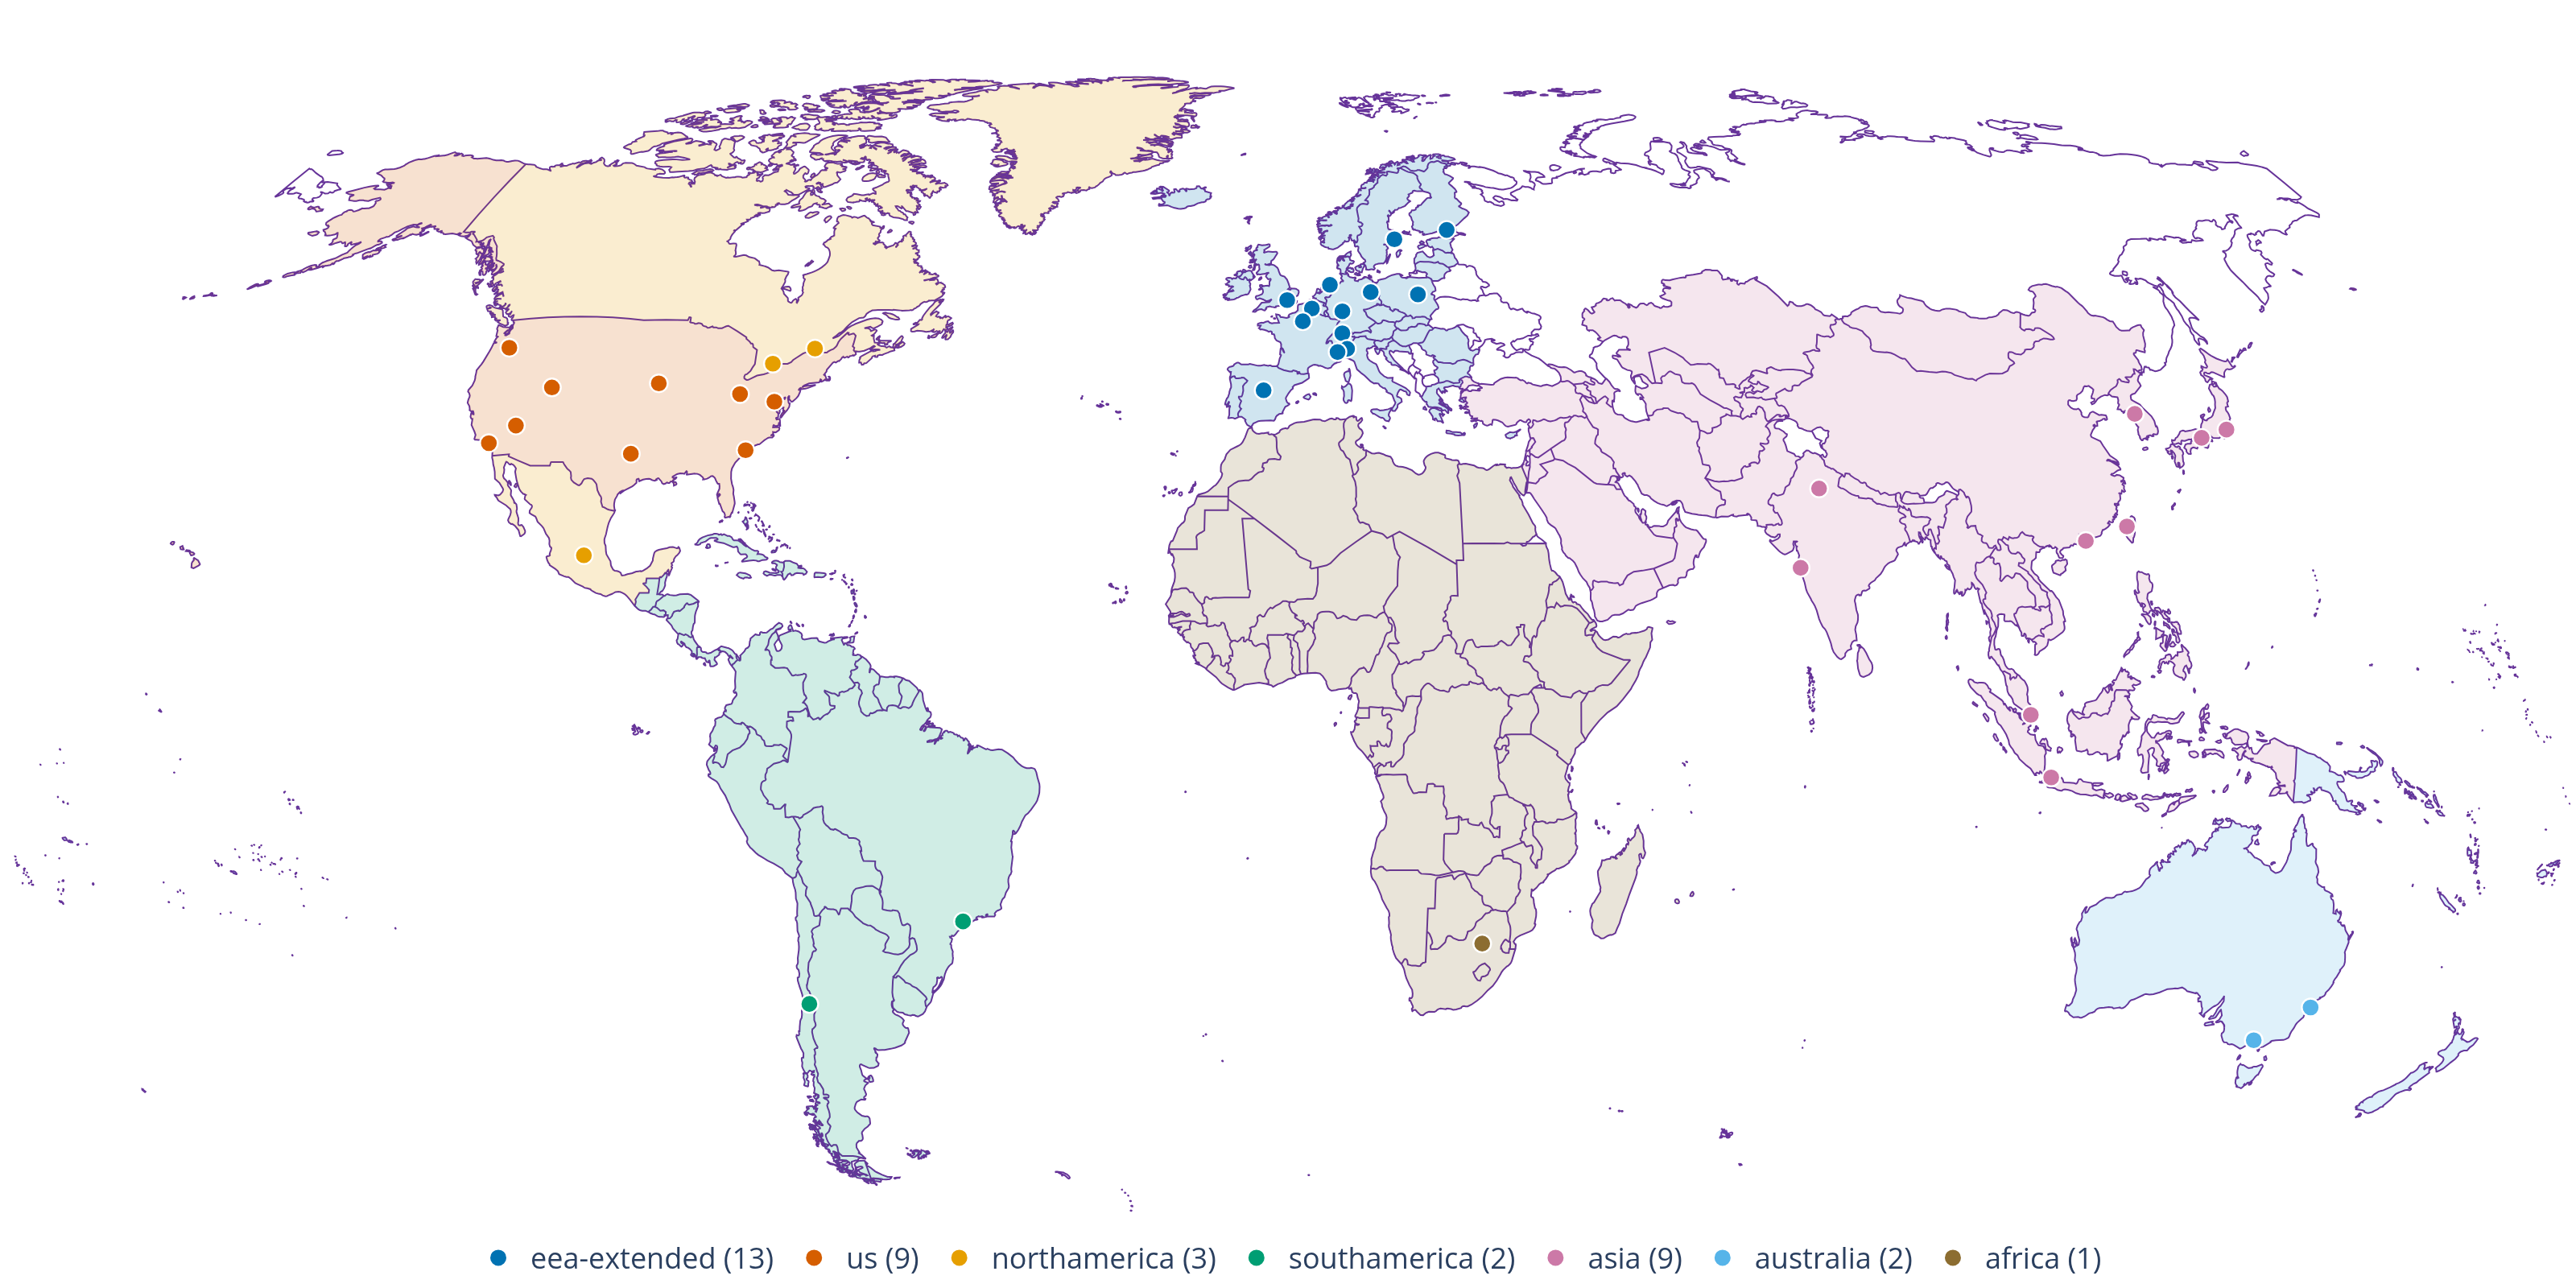
\includegraphics[width=\textwidth]{figures/images/rcadns_gc_locations_map.png}
    \caption{Google Cloud locations used in the RCA-DNS prototype, coloured according to the regional deployment to which they belong.}
    \label{fig:rcadns_gc_map}
\end{figure}

\subsection{Measurement Methodology}
\label{sc:rcadns_methodology}

Latency was measured with RIPE Atlas. Up to five probes were randomly selected in every country, subject to probe availability, so that both users inside and outside each region were represented. Figure~\ref{fig:rcadns_probes_map} shows the location of the probes that took part in the campaign. The measurements were conducted between 21 and 28 July 2026, that is, over eight consecutive days, at eight-hour intervals. In each round, every probe issued an HTTP request to the global name and to each of the seven regional names, and the round-trip time (RTT) of the HTTP transaction reported by RIPE Atlas was recorded. RTT was selected as the primary metric because it captures both network propagation delay and server responsiveness, and therefore reflects the latency perceived by an application. In total, the campaign involved 644 probes in 182 countries and produced 104,377 valid measurements after discarding failed requests.

Each probe was assigned to a region according to the country in which it is located. The names of the regional deployments follow the naming of the Google Cloud regions they group, but the set of countries whose probes are considered inside each region is necessarily broader, since every country must be assigned to the deployment intended to serve it. Countries were assigned following the geographic regions of the United Nations M49 standard \cite{UNSDMethodology}, except for the two regions defined by legal criteria, \texttt{eea-extended} (the EEA together with the United Kingdom and Switzerland) and \texttt{us}, and for Mexico, which was assigned to \texttt{northamerica} because its Google Cloud location belongs to that region. Table~\ref{tab:rcadns_probe_regions} summarises the resulting assignment. As a consequence, \texttt{australia} covers the whole of Oceania, \texttt{southamerica} covers Latin America and the Caribbean, and \texttt{asia} also includes Western Asia, whose probes are served from other Asian locations because the Google Cloud locations in the Middle East were not part of the deployment. The assignment is geographic rather than jurisdictional: for instance, the French outermost regions, which are part of the European Union, are assigned to the region in which they are geographically located. Probes in countries not covered by any region, mainly European countries outside the EEA-Extended region, only contribute to the measurements taken from outside the regions.

\begin{table}[ht]
    \centering
    \small
    \caption{Countries whose probes are considered inside each region in the evaluation.}
    \label{tab:rcadns_probe_regions}
    \begin{tabularx}{\textwidth}{>{\raggedright\arraybackslash}p{3.0cm} >{\raggedright\arraybackslash}X c}
        \toprule
        \textbf{Regional name} & \textbf{Probe countries} & \textbf{\#} \\
        \midrule
        \texttt{eea-extended} & EEA member states, United Kingdom, Switzerland, and Åland Islands & 33 \\
        \rowsep{3}
        \texttt{us} & United States & 1 \\
        \rowsep{3}
        \texttt{northamerica} & Canada, Mexico, Greenland, Bermuda, and Saint Pierre and Miquelon & 5 \\
        \rowsep{3}
        \texttt{southamerica} & Latin America and the Caribbean (M49), excluding Mexico & 49 \\
        \rowsep{3}
        \texttt{australia} & Oceania (M49) and United States Minor Outlying Islands & 28 \\
        \rowsep{3}
        \texttt{asia} & Asia (M49), including Western Asia & 50 \\
        \rowsep{3}
        \texttt{africa} & Africa (M49) & 59 \\
        \bottomrule
    \end{tabularx}
\end{table}

\begin{figure}[ht]
    \centering
    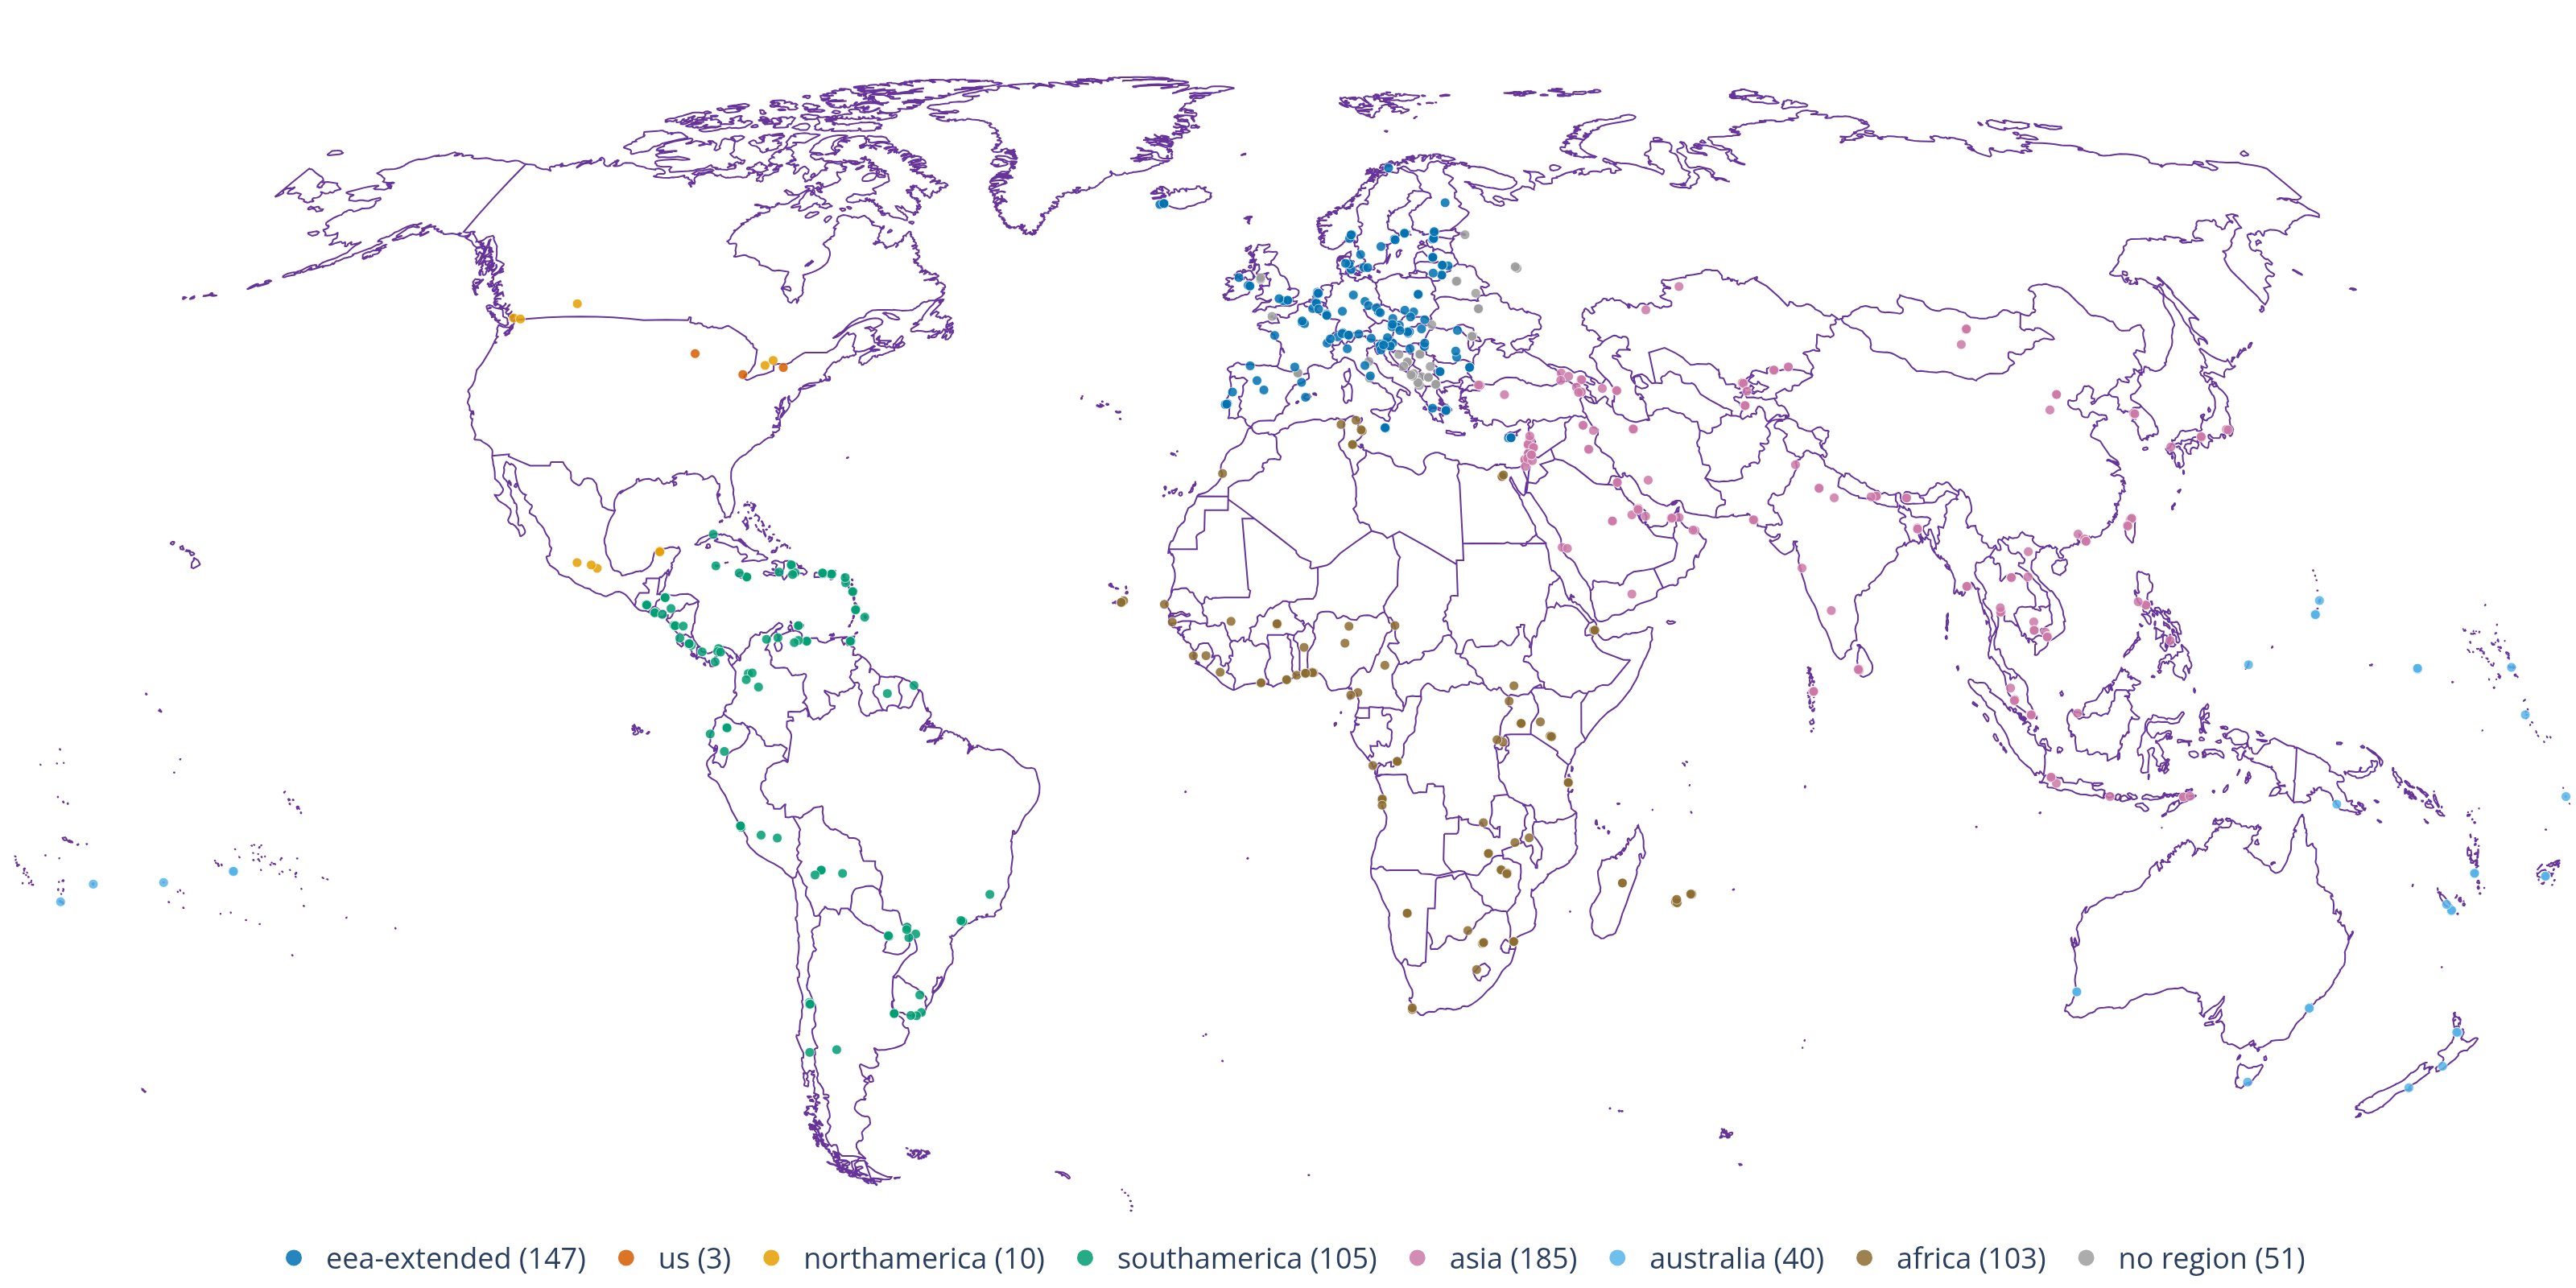
\includegraphics[width=\textwidth]{figures/images/rcadns_ripe_probes_map.png}
    \caption{Location of the RIPE Atlas probes used in the RCA-DNS evaluation.}
    \label{fig:rcadns_probes_map}
\end{figure}

\subsection{Results}
\label{sc:rcadns_results}

Table~\ref{tab:rcadns_median_rtt} compares, for each region, the median RTT observed by the probes located inside the region when accessing the service through its regional name and through the global name. The relative change is computed as $(\mathrm{RTT}_{\mathrm{global}} - \mathrm{RTT}_{\mathrm{regional}})/\mathrm{RTT}_{\mathrm{global}}$, so that positive values indicate that the regional deployment is faster and negative values that it is slower. Table~\ref{tab:rcadns_rtt_stats} complements the medians with the full distribution of the measurements.

\begin{table}[ht]
    \centering
    \small
    \caption{Median RTT observed by probes located inside each protected region when accessing the regional and the global deployments. Positive changes indicate that the regional deployment is faster.}
    \label{tab:rcadns_median_rtt}
    \begin{tabular}{lcccc}
        \toprule
        \textbf{Regional name} & \textbf{Locations} & \textbf{Regional RTT (ms)} & \textbf{Global RTT (ms)} & \textbf{Change} \\
        \midrule
        \texttt{eea-extended} & 13 & 47.98  & 51.03  & $+5.99\%$ \\
        \texttt{us}           &  9 & 153.05 & 145.31 & $-5.32\%$ \\
        \texttt{australia}    &  2 & 125.27 & 121.00 & $-3.53\%$ \\
        \texttt{northamerica} &  3 & 104.77 & 50.38  & $-107.94\%$ \\
        \texttt{africa}       &  1 & 369.87 & 143.34 & $-158.04\%$ \\
        \texttt{asia}         &  9 & 339.25 & 128.51 & $-163.99\%$ \\
        \texttt{southamerica} &  2 & 772.05 & 118.97 & $-548.92\%$ \\
        \bottomrule
    \end{tabular}
\end{table}

\begin{table}[ht]
    \centering
    \footnotesize
    \setlength{\tabcolsep}{4pt}
    \caption{Distribution of the RTT (ms) observed by probes located inside each region, for the regional (R) and global (G) names. $n$: number of valid measurements; $\leq$100~ms: percentage of measurements with an RTT of at most 100~ms.}
    \label{tab:rcadns_rtt_stats}
    \begin{tabular}{llrrrrrrrr}
        \toprule
        \textbf{Region} & & $n$ & \textbf{Min} & \textbf{P25} & \textbf{Median} & \textbf{P75} & \textbf{P95} & \textbf{Mean} & \textbf{$\leq$100 ms} \\
        \midrule
        \texttt{eea-extended}   & R & 3{,}026 & 10.44 & 33.44 & 47.98 & 69.84 & 111.25 & 61.60 & 93.2\% \\
                                & G & 3{,}019 & 11.01 & 35.17 & 51.03 & 80.33 & 1{,}252.37 & 197.59 & 86.8\% \\
        \rowsep{10}
        \texttt{us}             & R & 63 & 46.86 & 50.79 & 153.05 & 1{,}988.12 & 4{,}624.58 & 1{,}150.78 & 34.9\% \\
                                & G & 62 & 54.72 & 97.02 & 145.31 & 170.01 & 1{,}263.27 & 329.71 & 30.6\% \\
        \rowsep{10}
        \texttt{australia}      & R & 813 & 15.96 & 89.15 & 125.27 & 732.48 & 945.85 & 341.65 & 34.2\% \\
                                & G & 816 & 17.11 & 90.26 & 121.00 & 257.57 & 346.25 & 204.62 & 33.6\% \\
        \rowsep{10}
        \texttt{northamerica}   & R & 204 & 11.89 & 49.77 & 104.77 & 297.44 & 2{,}203.68 & 371.96 & 49.5\% \\
                                & G & 199 & 12.78 & 41.09 & 50.38 & 86.02 & 1{,}511.40 & 213.09 & 77.4\% \\
        \rowsep{10}
        \texttt{africa}         & R & 2{,}036 & 11.86 & 124.34 & 369.87 & 761.04 & 919.34 & 454.31 & 19.3\% \\
                                & G & 2{,}034 & 11.49 & 99.18 & 143.34 & 222.46 & 444.91 & 191.82 & 25.8\% \\
        \rowsep{10}
        \texttt{asia}           & R & 3{,}703 & 10.01 & 80.37 & 339.25 & 806.51 & 1{,}360.97 & 507.95 & 31.7\% \\
                                & G & 3{,}697 & 9.97 & 78.57 & 128.51 & 218.69 & 503.01 & 224.36 & 34.4\% \\
        \rowsep{10}
        \texttt{southamerica}   & R & 2{,}134 & 9.55 & 93.41 & 772.05 & 821.09 & 884.86 & 586.87 & 26.1\% \\
                                & G & 2{,}135 & 10.73 & 84.81 & 118.97 & 148.16 & 216.10 & 156.75 & 34.5\% \\
        \bottomrule
    \end{tabular}
\end{table}

\paragraph{Well-provisioned regions.} The results show that the performance impact of RCA-DNS is not uniform but depends primarily on the infrastructure available inside each region. EEA-Extended, with thirteen locations, is representative of a well-provisioned jurisdiction. Figure~\ref{fig:rcadns_cdf_eea} shows the cumulative distribution of the RTT observed by EEA-Extended probes for both names. The regional deployment not only preserves performance but improves it: the median RTT decreases by 5.99\% (47.98~ms versus 51.03~ms), and the mean decreases by 68.83\% (61.60~ms versus 197.59~ms). The 95th percentile makes this effect explicit: it remains at 111.25~ms for the regional deployment, whereas it reaches 1{,}252.37~ms for the global one. The large difference between the two means indicates that the global deployment produces a heavier tail of high-latency requests, which disappears when backend selection is restricted to the region. In other words, constraining traffic to the region eliminates detours that occur under the global deployment while maintaining the responsiveness expected from modern Internet services. The United States, with nine locations, and Australia, with two locations close to most of the population, show modest median increases of 5.32\% and 3.54\%, respectively. The results for the United States should, however, be interpreted with caution. Since probes were selected with the same criterion in every country (up to five per country), regions composed of many countries aggregate measurements from a large number of probes, whereas the US region, which corresponds to a single country, is represented by far fewer. As a result, it accumulates only 63 valid measurements, compared with several hundred or thousands in the other regions, and its upper percentiles are dominated by a few high-latency measurements (the 75th percentile reaches 1{,}988.12~ms for the regional name).

\begin{figure}[ht]
    \centering
    \begin{subfigure}{0.48\textwidth}
        \centering
        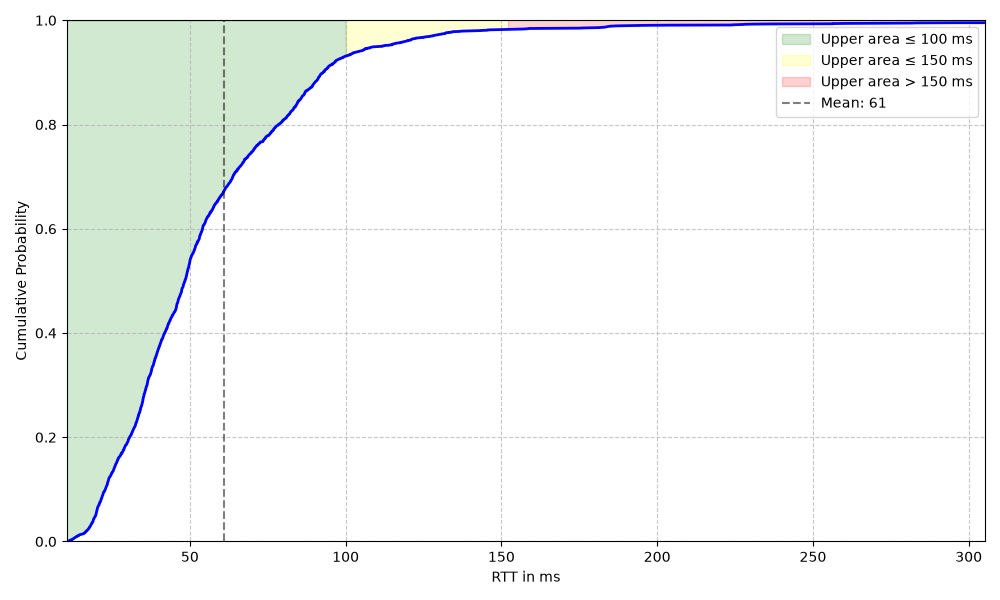
\includegraphics[width=\textwidth]{figures/images/figure_cdf_rtts_from_eea-extended_to_eea-extended.anycastprivacy.org.png}
        \caption{Regional (\texttt{eea-extended.anycastprivacy.org}).}
        \label{fig:rcadns_cdf_eea_regional}
    \end{subfigure}
    \hfill
    \begin{subfigure}{0.48\textwidth}
        \centering
        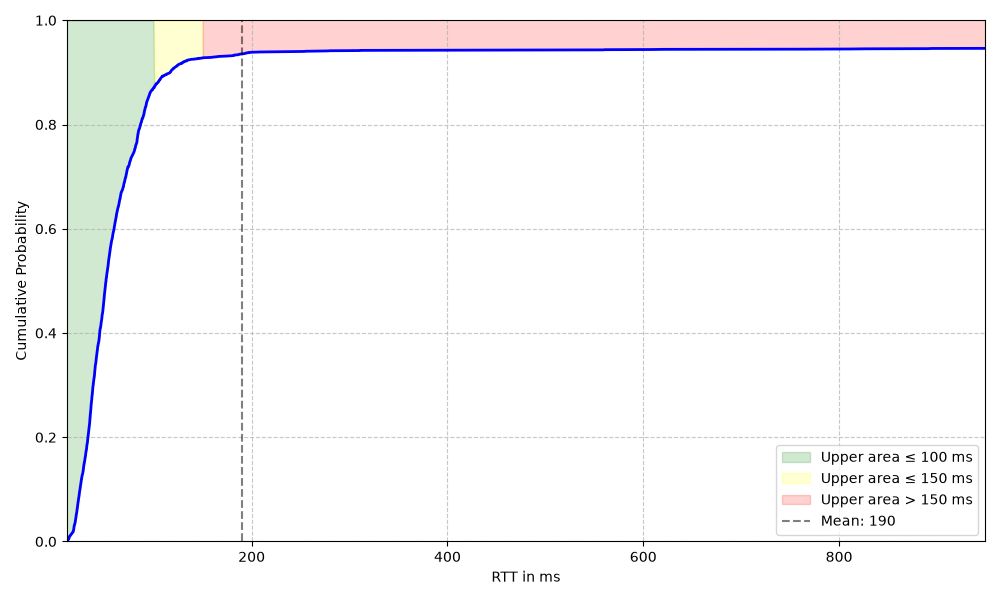
\includegraphics[width=\textwidth]{figures/images/figure_cdf_rtts_from_eea-extended_to_global.anycastprivacy.org.png}
        \caption{Global (\texttt{global.anycastprivacy.org}).}
        \label{fig:rcadns_cdf_eea_global}
    \end{subfigure}
    \caption{Cumulative distribution of the RTT observed by probes located in EEA-Extended countries when accessing the service through the regional deployment and through the conventional global deployment.}
    \label{fig:rcadns_cdf_eea}
\end{figure}

\paragraph{Sparsely provisioned regions.} Africa, South America, and Asia incur substantially larger penalties. In Africa and South America, the reason is the limited number of locations: all African probes must be served from Johannesburg, and all South American probes from São Paulo or Santiago, whereas the global deployment can serve many of them from closer locations in Europe or North America, or through better-connected routes. In South America, the median regional RTT (772.05~ms) is higher than the mean (586.87~ms) because the distribution is bimodal: a minority of measurements, mostly from probes close to the São Paulo and Santiago locations, achieve low latencies (the 25th percentile is 93.41~ms), while the majority concentrate around 800~ms (the 75th percentile is 821.09~ms). Asia illustrates a different effect. Although it has nine locations, the region spans a very large area, and the paths from many Asian countries to locations within the region are longer than the paths that the global deployment can use towards locations in other regions. North America (Canada and Mexico) is a similar case, since a large fraction of its users is closer to locations in the United States than to Toronto, Montreal, or Mexico. 

These results show that the latency cost of jurisdictional confinement is determined by the availability and distribution of infrastructure within the protected region rather than by the RCA-DNS mechanism itself. Where providers offer dense regional footprints, confinement is obtained at no cost or even with a performance gain; where they do not, the cost is the price of not being able to use infrastructure located in other jurisdictions. This trade-off is inherent to any form of data localisation, but RCA-DNS makes it explicit and allows each service to decide, region by region, whether to accept it.

\paragraph{Users outside the protected region.} Users located outside a region who are nevertheless assigned to it, such as a European resident travelling abroad, bear the cost of confinement. For instance, probes located outside the EEA-Extended region observed a median RTT of 348.94~ms when accessing \texttt{eea-extended.anycastprivacy.org}, compared with 47.98~ms for probes inside the region. This cost is inherent to the policy rather than to the mechanism: if a service requires that the communications of a user be processed in the EEA, they must reach EEA infrastructure wherever the user is.

% ============================================================
\section{Discussion and Limitations}
\label{sc:rcadns_discussion}
% ============================================================

\subsection{Regulatory Implications}
\label{sc:rcadns_discussion_regulatory}

RCA-DNS addresses the central problem identified in this thesis: conventional anycast deployments offer no explicit control over the jurisdictions in which communications are processed. By turning the region into an explicit parameter of each communication, RCA-DNS allows a service provider to know, and to demonstrate, where personal data is processed. This supports both the transparency obligations discussed in Chapter~\ref{ch:experiments}, since the jurisdictions disclosed in a privacy policy can now be enforced rather than merely estimated, and the accountability principle of the GDPR, under which controllers must be able to demonstrate compliance.

From a GDPR perspective, RCA-DNS is an instance of \textit{data protection by design and by default} (Article~25) \cite{REGULATIONSRelevance, GuidelinesBoard}. Article~25 requires controllers to implement appropriate technical measures, both when determining the means of processing and at the time of the processing itself, that effectively implement data protection principles. RCA-DNS is such a measure: it embeds the geographic restriction in the architecture of the service instead of relying on organisational commitments, it does not introduce new processing of personal data (the region can be derived from information the service already holds), and, with the default configuration of a region-restricted name, it ensures that communications are not transferred outside the region unless the service explicitly decides otherwise. The fail-closed behaviour described in Section~\ref{sc:rcadns_operations} is a direct expression of protection by default.

\subsection{Requirements Revisited}
\label{sc:rcadns_discussion_requirements}

Once a region is selected, the location-independent mapping of names to addresses and the restriction of each address to in-region infrastructure make confinement deterministic (R1), with the strength of the guarantee determined by the enforcement level discussed in Section~\ref{sc:rcadns_enforcement}. The architecture only uses DNS records and anycast deployments that are standard on all the analysed platforms (R2), and each service can adopt it on its own (R3). Load distribution, failover, and the selection of nearby replicas continue to be performed by anycast within each region (R4), with the latency results of Section~\ref{sc:rcadns_results} showing that the benefits are preserved wherever the regional footprint is adequate. The deployment is managed with the standard tools of the provider (R5), and regions can be defined as arbitrary sets of locations while the selection rule remains under the control of the service (R6).

\subsection{Limitations}
\label{sc:rcadns_discussion_limitations}

\paragraph{Dependence on regional infrastructure.} The protection and performance offered by RCA-DNS in a region are bounded by the number and distribution of locations available there. As discussed in Section~\ref{sc:rcadns_feasibility_footprint}, this is a real constraint for regions such as Africa or South America on Google Cloud, but not for the EEA, the United States, or Asia, where providers already offer many locations. It can be mitigated by combining providers or by using CDNs with denser regional footprints.

\paragraph{Network path versus processing location.} RCA-DNS controls where communications are terminated and processed, not the physical path that packets follow across the Internet, which remains determined by inter-domain routing. As argued in Section~\ref{sc:rcadns_enforcement}, this residual exposure is addressed by HTTPS when TLS is only terminated inside the region, a situation that European data protection authorities consider an effective safeguard for data merely transiting third countries \cite{RecommendationsBoard}. Deployments that rely on edge proxies terminating TLS outside the region, as in enforcement level (a), should either restrict TLS termination to the region or carefully assess whether the edge provider's access to the data is acceptable.

\paragraph{Correctness of region determination.} RCA-DNS guarantees that the selected region is respected, but not that the right region is selected. However, RCA-DNS is not immune (as anyway expected) to providers' errors or misconfigurations e.g. if selecting an incorrect policy or relying on inaccurate users' geolocation. Such cases would result in a communication being confined to the wrong region. Since region determination is the responsibility of the service, it remains part of the compliance assessment that each service must carry out, and its study is left outside the scope of this thesis.

\paragraph{Experimental scope.} The design of the evaluation involves several decisions that limit its scope. Each of them is described below, together with the reasons that motivated it, its impact on the results, and the way in which it could be addressed.

\begin{itemize}
    \item \textbf{Single provider and enforcement level (a).} The prototype was deployed on a single provider, Google Cloud, using global layer-7 load balancers, which correspond to enforcement level (a) and therefore do not offer the strongest geographic guarantees. This choice was made because the objective of the evaluation is to quantify the latency impact of restricting backend selection to a region, and Google Cloud allowed building the regional and the global deployments on exactly the same edge network, backends, and software, so that any difference between them can be attributed to the geographic constraint alone. For users located inside the protected region, who are the focus of the evaluation, the results are also representative of levels (b) and (c): the closest point of presence is generally already inside the region, and in all three levels the request must reach a regional backend. For users outside the region, levels (b) and (c) would add latency, since the connection would be established with an endpoint inside the region rather than at the nearest edge, so the results of level (a) constitute a lower bound for them. Evaluating deployments at levels (b) and (c) on other providers would confirm these results with stronger guarantees and is part of the future work outlined in Chapter~\ref{ch:conclusion}.

    \item \textbf{Use of plain HTTP.} The measurements used plain HTTP instead of HTTPS for two reasons. First, the HTTP measurements of RIPE Atlas do not support HTTPS. Second, avoiding encryption keeps the service lightweight and prevents the cryptographic processing time from adding variability to the measured latency. This decision does not affect the comparison: with HTTPS, the TLS handshake would add the same number of round trips to both the regional and the global deployments, which terminate connections at the same edge in level (a). Measuring with HTTPS would require a measurement platform other than RIPE Atlas, at the cost of losing its geographic coverage.

    \item \textbf{Duration and probe coverage.} The campaign lasted eight days, and the probes were selected at random among those available in each country. The coverage of RIPE Atlas is uneven, so regions with few probes are less represented. RIPE Atlas was nevertheless chosen because it is the platform with the widest geographic distribution of vantage points available to researchers, which is essential to compare users located inside and outside each region. The duration was sufficient to capture daily variations, since each probe performed measurements at different times of the day throughout the campaign. Longer campaigns and complementary measurement platforms would increase the representativeness of the results in regions with few probes.

    \item \textbf{Uneven sample sizes across regions.} Selecting the same number of probes in every country yields uneven sample sizes across regions: single-country regions such as the United States are represented by far fewer measurements than regions spanning many countries, which limits the statistical robustness of their results. This criterion was adopted so that every country was represented under the same conditions, which is appropriate for analysing users located outside each region, but it penalises single-country regions. The results for the United States are therefore interpreted with caution in Section~\ref{sc:rcadns_results}. A selection proportional to the population or to the number of available probes in each region would provide more balanced samples in future campaigns.

    \item \textbf{Absence of production conditions.} The prototype was not subjected to production traffic, failures, or attacks, since the evaluation focused on the latency cost of confinement under normal operating conditions. Within each region, failover and attack absorption are handled by the same anycast mechanisms as in a conventional deployment, so RCA-DNS is not expected to alter them, but the reduced number of replicas in sparsely provisioned regions could limit them. Evaluating the behaviour of RCA-DNS under failures and high load is part of the future work outlined in Chapter~\ref{ch:conclusion}.
\end{itemize}

% ============================================================
\section{Summary and Next Steps}
\label{sc:rcadns_summary}
% ============================================================

This chapter has presented RCA-DNS, an architecture that \DIFdelbegin \DIFdel{introduces deterministic geographic control into anycast services }\DIFdelend \DIFaddbegin \DIFadd{allows anycast services to confine communications to selected regions }\DIFaddend by exposing one DNS name and one anycast address per region and by letting only in-region infrastructure serve each address. The region is selected by the service before DNS resolution, according to its own policy, while \DIFdelbegin \DIFdel{delivery }\DIFdelend \DIFaddbegin \DIFadd{traffic }\DIFaddend within the region \DIFdelbegin \DIFdel{remains in the hands of }\DIFdelend \DIFaddbegin \DIFadd{continues to follow }\DIFaddend conventional anycast routing. The \DIFaddbegin \DIFadd{strength of this confinement depends on the enforcement level at which it is implemented, which in turn depends on where each platform terminates TLS. The }\DIFaddend analysis of existing approaches has shown that none of \DIFdelbegin \DIFdel{them }\DIFdelend \DIFaddbegin \DIFadd{those reviewed }\DIFaddend combines deterministic confinement, the benefits of anycast, and service-defined policies\DIFdelbegin \DIFdel{. The }\DIFdelend \DIFaddbegin \DIFadd{, and the }\DIFaddend feasibility analysis has shown that the architecture can be implemented \DIFdelbegin \DIFdel{today }\DIFdelend on the main cloud and CDN platforms\DIFdelbegin \DIFdel{, with different levels of enforcement depending on where each platform terminates TLS}\DIFdelend . Finally, the evaluation of a prototype deployed in 39 Google Cloud locations \DIFdelbegin \DIFdel{has shown }\DIFdelend \DIFaddbegin \DIFadd{showed }\DIFaddend that, where regional infrastructure is dense, as in the EEA, confinement \DIFdelbegin \DIFdel{comes at no latency cost and even removes }\DIFdelend \DIFaddbegin \DIFadd{did not increase the median latency and substantially reduced }\DIFaddend the high-latency tail \DIFdelbegin \DIFdel{produced by global anycast}\DIFdelend \DIFaddbegin \DIFadd{observed with the global deployment}\DIFaddend , whereas in sparsely provisioned regions the \DIFdelbegin \DIFdel{cost reflects }\DIFdelend \DIFaddbegin \DIFadd{latency penalty is mainly explained by }\DIFaddend the lack of local infrastructure\DIFdelbegin \DIFdel{rather than the mechanism itself}\DIFdelend .

Taken together, these results answer RQ4: geographic control and anycast are not inherently incompatible. The tension between them arises from deployments that leave geographic constraints implicit, and it can be resolved by making the region an explicit, service-controlled parameter of each communication without modifying the routing infrastructure of the Internet. The contents of this chapter have been submitted for publication in the article \textit{Where does your data really go? Rethinking Geographic Control in Anycast systems}, which is under review at the moment of writing this document.

With RCA-DNS, the thesis completes the transition from observing the geographic behaviour of anycast communications to controlling it. Chapter~\ref{ch:conclusion} brings together the results of the three contribution chapters, discusses how they address the research questions, and outlines the limitations of this work and the lines of research that remain open, including the evaluation of RCA-DNS on other providers and its combination with Hunter to independently audit regional deployments. \newpage 
 \newpage \chapter{Conclusions}
\label{ch:conclusion}

This thesis investigated the implications of anycast routing for data sovereignty, international data transfers, and geographic control over Internet communications. The results demonstrate that anycast infrastructures introduce important challenges for transparency and geographic predictability, particularly in regulatory environments where the jurisdiction of personal data destination is a relevant consideration. At the same time, the thesis shows that these challenges can be measured, analysed, and addressed through appropriate measurement and architectural mechanisms.

This chapter summarises the main contributions of the thesis, evaluates the fulfilment of the research objectives, discusses the principal limitations of the conducted work, and outlines several directions for future research.

% ============================================================
\section{Research Objectives and Main Findings}
\label{sc:conclusion_objectives}
% ============================================================

Anycast routing plays a fundamental role in modern Internet infrastructures, yet its implications for data sovereignty, international data transfers, and geographic control have received comparatively limited attention. The research presented in this thesis addresses this gap by studying the geographic behaviour of anycast communications and its consequences for transparency, regulatory compliance, and jurisdictional exposure.

To address this gap, the first objective of the thesis was to determine whether the actual destination country of communications towards anycast infrastructures can be inferred with sufficient accuracy. The results presented in Chapter~\ref{ch:hunter} demonstrate that this objective was achieved successfully through the design and validation of Hunter, a methodology capable of estimating the geographic destination of anycast communications using active network measurements and routing analysis techniques.

The second objective was to quantify the impact of anycast on privacy and regulatory compliance. The large-scale analysis presented in Chapter~\ref{ch:experiments} identified 195,786 communications containing personal data and targeting anycast IP addresses, corresponding to 80.74\% of the communications containing personal data observed during the dynamic analysis. These communications frequently reached destinations outside the EEA: 195 of the 200 anycast IP addresses identified (97.5\%) were associated with at least one non-EEA destination (Section~\ref{sc:anycast_experiments_non_eea}). However, 98.65\% of the analysed applications did not explicitly disclose these destinations in their privacy policies (Section~\ref{sc:anycast_experiments_undisclosed}), revealing a substantial gap between the \DIFdelbegin \DIFdel{transfers declared }\DIFdelend \DIFaddbegin \DIFadd{destinations disclosed }\DIFaddend to users and those \DIFdelbegin \DIFdel{actually observed}\DIFdelend \DIFaddbegin \DIFadd{observed, which points to potential transparency gaps rather than established non-compliance}\DIFaddend . The global measurement campaign showed that this exposure is not limited to the Android ecosystem or to Europe, but is a common property of operational anycast deployments: 58.36\% of the valid routing tracks terminated in a country different from the one in which they originated, and 99.49\% of the analysed anycast addresses exhibited at least one cross-border routing event (Section~\ref{sc:anycast_experiments_global_anycast}).

The third objective was to analyse the role of software ecosystems and external dependencies in international data transfers. The analysis of TPLs presented in Section~\ref{sc:anycast_experiments_tpls} identified 20 TPLs that triggered 61,443 communications containing personal data towards anycast infrastructures, corresponding to 31.38\% of the analysed communications. These libraries were embedded in 606 of the 960 applications that generated such communications (63.13\%), which shows that a large share of the \DIFdelbegin \DIFdel{international transfers }\DIFdelend \DIFaddbegin \DIFadd{cross-border personal-data communications }\DIFaddend observed originate from components that application developers integrate but do not control. Moreover, although all the identified TPLs \DIFdelbegin \DIFdel{were involved in transfers }\DIFdelend \DIFaddbegin \DIFadd{generated communications }\DIFaddend that could reach destinations outside the EEA, 90\% of them \DIFdelbegin \DIFdel{potentially failed to }\DIFdelend \DIFaddbegin \DIFadd{did not }\DIFaddend disclose the destination countries, so the transparency gap identified for applications extends to the software supply chain on which they depend.

Finally, the thesis sought to determine whether geographic control could be achieved without abandoning the operational benefits of anycast. The RCA-DNS architecture presented in Chapter~\ref{ch:rcadns} demonstrated that making the region an explicit parameter of each communication, selected by the service before DNS resolution, deterministically restricts anycast communications to the infrastructure of the selected region, while load distribution and failover within the region continue to be handled by anycast. The evaluation of a prototype deployed in 39 Google Cloud locations showed that, where regional infrastructure is dense, as in the EEA, confinement \DIFdelbegin \DIFdel{comes at no latencycost}\DIFdelend \DIFaddbegin \DIFadd{did not increase latency}\DIFaddend : the median RTT decreased by 5.99\% and the 95th percentile dropped from 1{,}252.37~ms to 111.25~ms compared with a global deployment on the same infrastructure. In sparsely provisioned regions, the latency penalty \DIFdelbegin \DIFdel{reflects }\DIFdelend \DIFaddbegin \DIFadd{is mainly explained by }\DIFaddend the lack of local infrastructure\DIFdelbegin \DIFdel{rather than the mechanism itself}\DIFdelend .

The results obtained throughout this research demonstrate that the geographic destination should not be regarded as a static property of anycast communications. Instead, it emerges as a dynamic characteristic influenced by routing decisions, network conditions, and infrastructure deployment strategies. Consequently, any meaningful assessment of data sovereignty and international transfers in anycast environments requires both visibility into routing behaviour and mechanisms capable of influencing geographic service selection.

% ============================================================
\section{Scientific Contributions}
\label{sc:conclusion_contributions}
% ============================================================

The research presented in this thesis contributes to the study of anycast infrastructures, geographic control, and data sovereignty through three complementary lines of work that span measurement, empirical analysis, and system design.

The first contribution is Hunter, a methodology for inferring the geographic destinations reached by communications towards anycast infrastructures. Hunter combines traceroute analysis, last-hop identification, latency-based multilateration, and geographic inference techniques to estimate the destination country associated with operational anycast deployments. The validation results \DIFdelbegin \DIFdel{demonstrate }\DIFdelend \DIFaddbegin \DIFadd{show }\DIFaddend that the proposed methodology achieves \DIFdelbegin \DIFdel{high levels of accuracy }\DIFdelend \DIFaddbegin \DIFadd{a high precision }\DIFaddend while remaining applicable at Internet scale. By providing visibility into the geographic behaviour of anycast communications, Hunter enables systematic analysis of geographic destinations that would otherwise be difficult to observe.

The second contribution consists of a large-scale empirical analysis of \DIFdelbegin \DIFdel{international personal data transfers }\DIFdelend \DIFaddbegin \DIFadd{cross-border personal-data communications }\DIFaddend involving anycast infrastructures in Android applications. By combining dynamic traffic analysis, privacy policy inspection, and anycast destination inference, the study provides empirical evidence of the geographic exposure associated with anycast communications carrying personal data. The analysis also characterises the discrepancy between the jurisdictions reached in practice and those disclosed to users, and examines the role of TPLs in these communications. In particular, the results show that jurisdictional exposure extends across multiple applications, services, and TPLs, providing an empirical basis for analysing the implications of anycast routing for transparency and data sovereignty.

The third contribution is the design and experimental evaluation of Region-Constrained Anycast over DNS (RCA-DNS), a practical architecture for introducing geographic constraints into anycast service deployments. The proposed approach combines DNS-based service selection with geographically scoped anycast infrastructures, allowing service providers to enforce geographic constraints on the jurisdictions reached by user communications while preserving the operational benefits of anycast. The experimental evaluation showed that \DIFdelbegin \DIFdel{geographic confinement can be achieved while maintaining latency levels compatible with modern Internet services, demonstrating the practical feasibility of jurisdiction-aware anycast deployments}\DIFdelend \DIFaddbegin \DIFadd{the latency cost of confinement depends on the infrastructure available in each region: it is negligible, or even negative, in well-provisioned regions such as the EEA, and significant in regions with few locations}\DIFaddend .

Taken together, these contributions establish a research framework that connects the measurement of geographic routing behaviour with the empirical analysis of its consequences and the design of mechanisms capable of enforcing geographic constraints. The thesis therefore moves from observing and characterising jurisdictional exposure to providing an architectural approach for controlling it. This perspective extends the traditional understanding of anycast by treating geographic destination as an operational property that can be measured, analysed, and, under appropriate architectural constraints, controlled.

% ============================================================
\section{Impact of the Research}
\label{sc:conclusion_impact}
% ============================================================

The research conducted throughout this thesis has also contributed to a broader set of scientific activities, including research collaborations, scientific publications, international research activities, and the supervision of student projects. These activities have provided opportunities to disseminate the results of the thesis, apply the knowledge developed to related research problems, and contribute to the training of other researchers.

\subsection{Research Projects and Collaborations}
\label{sc:conclusion_projects}

The work developed during this thesis has been carried out within the context of several national and European research projects. These collaborations provided opportunities to apply the concepts and techniques developed in this thesis to related problems involving data protection, distributed infrastructures, data spaces, and digital services.

The research activities were conducted in collaboration with the projects \emph{AutoGDPR -- Evaluación automática del cumplimiento del Reglamento General de Protección de Datos} (TED2021-130455A-I00), funded by the Spanish Ministry of Science and Innovation through the State Research Agency and the European Union NextGenerationEU programme; \emph{Re-InitS} project, funded by the Plan Estatal de Investigación Científica y Técnica y de Innovación 2024-2027 (Ministerio de Ciencia e Investigación (Spain) - MCIN/AEI/10.13039/501100011033) under grant agreement PID2024-155230OB-C43.; \emph{ACES -- Autopoietic Cognitive Edge-Cloud Services} (HORIZON-CL4-2022-DATA-01, project 101093126), funded by the European Union through the European Commission; \emph{CEDAR -- Common European Data Spaces and Robust AI for Transparent Public Governance} (HORIZON-CL4-2023-DATA-01, project 101135577), funded by the European Union through the European Commission; and \emph{EDACCIT -- Espacio de Datos de Cambio Climático en Infraestructuras de Transporte} (TSI-100123-2024-0007), funded by the Spanish Ministry for Digital Transformation and Public Administration.

The participation in these projects contributed to extending the scope of the research beyond the specific problems addressed in this thesis and facilitated collaboration with researchers working on related challenges in privacy, data governance, distributed infrastructures, and data spaces.

\subsection{Scientific Dissemination}
\label{sc:conclusion_dissemination}

The research presented in this thesis has resulted in two scientific publications that address the main contributions developed throughout the work. The research on the geographic inference of anycast communications resulted in the publication \emph{Hunter: Tracing anycast communications to uncover cross-border personal data transfers} \cite{Pascual2024Hunter:Transfers}, published in \emph{Computers \& Security} in June 2024. The journal is ranked 42nd out of 258 journals in the 2024 Journal Impact Factor (JIF) ranking and is classified in Q1. The analysis of the relationship between anycast infrastructures, TPLs, and privacy resulted in the publication \emph{Anycast and Third-party Libraries: A Recipe for a Privacy Disaster?} \cite{Pascual2025AnycastDisaster}, published in \emph{IEEE Communications Magazine} in March 2025. The journal is ranked 14th out of 127 journals in the 2025 Journal Impact Factor (JIF) ranking and is classified in Q1. Together, these publications disseminated the main methodologies, analyses, and empirical findings developed throughout this thesis to the research community. In addition, the RCA-DNS architecture presented in Chapter~\ref{ch:rcadns} is described in the manuscript \emph{Where does your data really go? Rethinking Geographic Control in Anycast systems}, which, at the time of writing, is under review at a Q1 journal.

The research presented in this thesis has also been disseminated through several international scientific events. In August 2023, the work was presented at the 18th International IFIP Summer School on Privacy and Identity Management in Oslo, Norway, including participation in an interdisciplinary workshop. In September 2024, the research contributed to the organisation of the 19th International IFIP Summer School on Privacy and Identity Management in Madrid, Spain. In July 2025, the research was presented under the title ``Is anycast a threat to privacy?'' at the Next Generation Networking, Multi-Service Networks Workshop in Abingdon, United Kingdom. The research activities were further complemented by attendance in NetUK2 in London, United Kingdom, and the 123rd IETF meeting in Madrid, Spain.

The dissemination activities were complemented by participation in the peer-review process of the scientific community. In particular, I served as a reviewer for the Smart Cities and Critical Infrastructures (SCCI) track of the 40th ACM Symposium on Applied Computing (SAC 2025), held in Catania, Italy.

\subsection{International Research Activities}
\label{sc:conclusion_internationalisation}

As part of the internationalisation of the research developed during this thesis, an international research stay was conducted at Queen Mary University of London from 6 May to 13 August of 2025. The stay provided an opportunity to collaborate with researchers in an international academic environment and to extend the research developed throughout the thesis to related problems. The research conducted during this period resulted in the design of the RCA-DNS architecture presented in Chapter~\ref{ch:rcadns}, which is described in a manuscript that, at the time of writing, is under review at a Q1 journal.

\subsection{Supervised Student Projects}
\label{sc:conclusion_student_projects}

The research activities developed during the thesis also provided a basis for supervising student projects related to the broader research topics addressed in this work. One example is the Bachelor's Thesis ``Identity Control in Heterogeneous Systems'', which investigated the integration of centralised identity and access management mechanisms in distributed infrastructures. The project evaluated open-source technologies for identity management, authentication, access policies, auditing, and Single Sign-On, and considered their deployment in a containerised environment with requirements for scalability, availability, and resilience.

Although this project addresses a specific problem different from the main research questions in this thesis, it is related to the broader themes of distributed infrastructure management, security, and controlled access to digital services. Its development also provided an opportunity to transfer the knowledge and methodologies developed during the research to the supervision and training of undergraduate students.

% ============================================================
\section{Limitations}
\label{sc:conclusion_limitations}
% ============================================================

The destination inference methodology developed in this thesis relies on active network measurements and geolocation information. As discussed throughout Chapter~\ref{ch:hunter}, although Hunter achieved high accuracy and precision during its validation, destination inference remains inherently dependent on the quality of the underlying measurement data and geolocation sources. Internet routing dynamics, incomplete measurement visibility, and inaccuracies in public geolocation databases may affect individual inferences. Nevertheless, the large-scale nature of the experiments and the repeated measurements performed throughout the study mitigate the impact of isolated errors on the overall conclusions.

\DIFaddbegin \DIFadd{Moreover, Hunter infers the country of the last element of the IP-level connection, which, when the service relies on a cloud or CDN provider, may not coincide with the place where its content is decrypted or processed. In layer-7 infrastructures, the inferred country is the first location where the content is available in clear, and therefore a lower bound of the jurisdictions involved; in layer-4 infrastructures, it may be a location where only connection metadata are handled. Since the configuration of each service is not visible from outside, this distinction cannot be resolved for individual services. Finally, the measurements presented in this thesis provide the technical evidence on which the legal assessment of each communication can be built: where communications terminate and whether these destinations are disclosed to users. Completing that assessment, that is, determining whether a specific communication constitutes an international transfer and which safeguards apply to it, additionally requires information about the entities involved that controllers hold and network measurements cannot provide. Both perspectives are therefore complementary, and the methods developed in this thesis allow controllers, auditors, and authorities to contrast declared data flows with the actual behaviour of the network.
}

\DIFaddend The large-scale analysis of Android applications was based on dynamic execution techniques. As with any dynamic analysis methodology, complete behavioural coverage cannot be guaranteed. Certain application functionalities may only be triggered under specific user interactions, authentication requirements, geographic conditions, or runtime contexts that were not reproduced during the experiments. Consequently, the observed communications should be interpreted as a lower bound of the actual \DIFdelbegin \DIFdel{data transfers }\DIFdelend \DIFaddbegin \DIFadd{communications }\DIFaddend performed by the analysed applications and TPLs.

The privacy policy analysis focused on identifying the jurisdictions disclosed as possible destinations for international transfers. While the methodology enabled a systematic comparison between declared and observed destinations, privacy policies often contain ambiguous language, generic statements, or references to external providers that complicate automated interpretation. Furthermore, privacy documentation may evolve over time, potentially introducing changes after the measurements were conducted.

The global measurements performed using Hunter were necessarily constrained by the availability and geographic distribution of measurement vantage points. Although RIPE Atlas provided broad coverage across the studied regions, certain countries and networks remain under-represented. Consequently, the observed routing behaviours may not capture every possible destination reachable through a given anycast deployment.

The evaluation of RCA-DNS was conducted on a single provider, Google Cloud, using a deployment that confines processing to the selected region but terminates connections at the provider's global edge, which corresponds to the weakest of the enforcement levels discussed in Chapter~\ref{ch:rcadns}. Although the prototype covered 39 locations grouped into seven regions, the protection and performance it offers in each region are bounded by the infrastructure available there, which remains limited in regions such as Africa or South America. The measurement campaign lasted eight days, used plain HTTP, and selected the same number of probes in every country, which yields uneven sample sizes across regions and limits the robustness of the results for single-country regions such as the United States. Moreover, the evaluation concentrated on latency, leaving aspects such as resilience under failures, behaviour under production traffic, and resistance to attacks outside the scope of the study. Finally, RCA-DNS guarantees that the selected region is respected but not that the right region is selected, since region determination is left to each service.

Despite these limitations, the methodologies, measurements, and analyses presented throughout this thesis consistently reveal a previously underexplored relationship between anycast routing, \DIFdelbegin \DIFdel{international datatransfers}\DIFdelend \DIFaddbegin \DIFadd{cross-border communications of personal data}\DIFaddend , and geographic control. Although the exact magnitude of the observed phenomena may vary under different experimental conditions, the results obtained across multiple datasets, measurement campaigns, and methodological approaches provide consistent evidence supporting the main conclusions of this thesis. Taken together, these findings provide strong evidence that geographic destination is a dynamic property of anycast communications and that routing behaviour must be considered when analysing data sovereignty and jurisdictional exposure in modern Internet infrastructures.

% ============================================================
\section{Future Research Directions}
\label{sc:conclusion_future}
% ============================================================

The destination inference methodology developed in this thesis can be extended in several directions. Although Hunter demonstrated high accuracy in identifying the destination countries of anycast communications, additional improvements could be achieved by incorporating new measurement sources, routing datasets, or geolocation techniques. Future work could also investigate mechanisms for continuously monitoring anycast deployments and automatically detecting changes in their geographic footprint over time. Such capabilities would be particularly valuable for organisations seeking to assess jurisdictional exposure in dynamic network environments.

The large-scale analysis presented in this thesis focused on the Android ecosystem due to its widespread adoption and extensive reliance on cloud-based services and TPLs. However, the same methodology could be applied to other environments, including web applications, Internet of Things platforms, content delivery systems, and cloud-native services. Extending the analysis to these domains would provide a broader understanding of how anycast infrastructures influence cross-border communications across the Internet.

The transparency challenges identified throughout Chapter~\ref{ch:experiments} also motivate further research into mechanisms capable of communicating geographic processing locations and jurisdictional exposure more effectively. Current privacy policies typically describe international transfers through static and high-level statements that are poorly suited to the dynamic nature of anycast routing. New approaches capable of representing destination variability and routing-induced geographic changes could improve the information available to users and organisations.

The relationship between anycast infrastructures and emerging regulatory requirements related to data sovereignty constitutes another promising area for future work. The results obtained throughout this thesis suggest that geographic destination should be considered a dynamic operational property rather than a fixed characteristic of a service. Consequently, compliance assessment methodologies, auditing processes, and regulatory frameworks may need to evolve in order to account for routing-induced geographic variability.

The RCA-DNS architecture presented in Chapter~\ref{ch:rcadns} represents an initial step towards jurisdiction-aware anycast deployments. Future evaluations should cover additional providers and, in particular, deployments that terminate TLS only inside the region or that confine the announcement of each regional prefix, which offer stronger guarantees than the prototype evaluated in this thesis. Evaluating the architecture under failure conditions, production traffic, and longer observation periods, with probe selections proportional to the population or to the probes available in each region, would provide a more complete understanding of the trade-offs between geographic confinement, performance, and availability.

Two aspects deliberately left outside the scope of RCA-DNS also deserve further research. The first is region determination: although regions defined by countries, adequacy decisions, or contractual criteria are already supported by the architecture, the mechanisms that assign each communication to a region, and the way they can be automated, audited, and kept up to date as contractual or regulatory conditions change, remain to be studied. The second is verification: destination inference techniques such as Hunter could be used to audit RCA-DNS deployments independently, checking from the outside that the communications directed to a regional name are actually terminated within the declared region. Combining both lines of work would close the loop between observing and controlling the geographic behaviour of anycast services.

Alternative approaches to geographic control also deserve further investigation. Integrating geographic awareness directly into routing decisions, traffic engineering policies, cloud orchestration platforms, or service deployment strategies may provide additional levels of control over the jurisdictions reached by Internet communications. Exploring these approaches could contribute to the development of Internet infrastructures capable of simultaneously satisfying performance, resilience, and geographic governance requirements.

More broadly, the results of this thesis suggest that geographic awareness is likely to become an increasingly important design consideration for distributed Internet services. As global infrastructures continue to expand and regulatory requirements surrounding data sovereignty evolve, understanding and controlling the geographic behaviour of networked systems will remain an important and challenging area of research.

% ============================================================
\section{Reproducibility and Open Science}
\label{sc:conclusion_reproducibility}
% ============================================================

Reproducibility and open science have been considered throughout the development of this thesis as part of the research methodology. In accordance with the Design Science Research approach adopted in this work and described in Section~\ref{sc:introduction_methodology}, the research process includes the development and evaluation of reusable artefacts that can support independent verification and further research. Consequently, whenever permitted by ethical, legal, and licensing constraints, the software, datasets, and experimental artefacts developed throughout this thesis have been made publicly available.

The availability of these resources facilitates independent verification of the results presented and enables other researchers to reuse the developed methodologies, extend the experiments to new scenarios, and investigate related problems involving anycast infrastructures, geographic control, and data sovereignty.

\subsection{Research Artefacts}
\label{sc:conclusion_research_artefacts}

Several software components, datasets, and experimental artefacts were developed throughout this thesis. The software developed as part of this work has been released as open-source software, while the datasets and other experimental artefacts have been made publicly available whenever permitted by the applicable conditions.

The first artefact is Hunter, the methodology and software implementation presented in Chapter~\ref{ch:hunter}. Hunter combines traceroute analysis, last-hop identification, latency-based multilateration, and geographic inference techniques to determine the destination country associated with communications towards anycast infrastructures. The implementation includes the algorithms used throughout the validation and experimental campaigns.

The second set of artefacts corresponds to the experimental deployment and evaluation of the RCA-DNS architecture presented in Chapter~\ref{ch:rcadns}. These artefacts include the deployment configuration, measurement procedures, scripts, and experimental data used to assess the feasibility and performance implications of geographically constrained anycast deployments.

Additional artefacts include the software developed to collect and process RIPE Atlas measurements, the analysis tools used throughout the Android traffic studies, and the software employed to correlate network measurements, destination inference results, and privacy policy information.

Several datasets generated during this work have also been preserved and released. These include the data collected during the Hunter validation, the measurement campaigns used to study jurisdictional exposure in operational anycast infrastructures, and the datasets associated with the Android traffic analysis experiments.

The complete source code of this dissertation, including the \LaTeX{} sources and the figures used throughout the manuscript, has also been maintained under version control in a public repository to facilitate transparency and long-term preservation.

\begin{table}[ht]
    \centering
    \small
    \caption{Publicly available artefacts associated with this thesis.}
    \label{tab:research_artefacts}
    \begin{tabularx}{\textwidth}{>{\raggedright\arraybackslash}p{6.2cm} >{\raggedright\arraybackslash}X}
        \toprule
        \textbf{Artefact} & \textbf{Repository / reference} \\
        \midrule
        Hunter source code & \url{https://github.com/STRAST-UPM/Hunter} \\
        \rowsep{2}
        Hunter validation analysis source code & \url{https://github.com/STRAST-UPM/hunter_cose_data} \\
        \rowsep{2}
        Hunter validation dataset & \url{https://doi.org/10.17632/ggnfwf5gw8.1} \\
        \rowsep{2}
        Europe anycast cross-border experiment source code & \url{https://github.com/STRAST-UPM/hunter_experiment_anycast_europe} \\
        \rowsep{2}
        Europe anycast cross-border experiment datasets & \url{https://doi.org/10.17632/7y627xjdzd.2} \\
        \rowsep{2}
        Global anycast cross-border experiment source code & \url{https://github.com/STRAST-UPM/experiments_hunter} \\
        \rowsep{2}
        Global anycast cross-border experiment datasets & \url{https://doi.org/10.17632/n93r278vzy.1} \\
        \rowsep{2}
        RCA-DNS deployment and evaluation source code & \url{https://github.com/STRAST-UPM/RCA-DNS} \\
        \rowsep{2}
        RCA-DNS evaluation datasets & \url{https://doi.org/10.17632/ntys787cys.1} \\
        \rowsep{2}
        Thesis source code & \url{https://github.com/hugopascual/anycast_privacy_thesis} \\
        \bottomrule
    \end{tabularx}
\end{table}

\subsection{Reproducibility Considerations}
\label{sc:conclusion_reproducibility_considerations}

The experiments presented throughout this thesis were designed to facilitate independent reproduction using publicly accessible infrastructures, open datasets, and standard measurement tools whenever possible. In particular, RIPE Atlas was used as the main measurement platform for Hunter's validation and for large-scale measurement campaigns, providing a publicly accessible infrastructure through which comparable measurements can be conducted.

The availability of the developed software and datasets enables the reproduction of the processing pipelines used in this work, from the analysis of raw measurements to the generation of the reported results and figures. These resources also allow the experiments to be extended to new measurement sources, geographic regions, or datasets.

Nevertheless, reproducibility in experiments on the Internet presents inherent challenges. Routing dynamics, changes in cloud deployments, modifications in RIPE Atlas probe availability, and the continuous evolution of Android applications mean that repeating an experiment at a different point in time may produce results that differ from those reported in this thesis. Such differences are an inherent characteristic of the dynamic Internet environment.

Therefore, reproducibility in this context should not be understood as obtaining identical measurements but rather as enabling independent researchers to execute the same methodologies, analyse comparable data, and assess whether the conclusions remain consistent under equivalent experimental conditions. The public availability of the software artefacts, datasets, and experimental procedures developed throughout this thesis provides a foundation for such independent verification and future research.

% ============================================================
\section{Closing Remarks}
\label{sc:conclusion_closing}
% ============================================================

Anycast has become a fundamental building block of modern Internet infrastructure. Its ability to improve performance, scalability, and resilience has led to its widespread adoption by cloud providers, content delivery networks, security services, and countless online platforms. However, as this thesis has shown, the geographic consequences of anycast routing extend beyond traditional networking concerns and directly influence where communications are processed and, ultimately, under which jurisdictions data may be exposed. In the current geopolitical context, data sovereignty has become an increasingly important strategic and legal concern, as control over the jurisdictions in which data is processed is closely linked to national autonomy, regulatory compliance, and the protection of sensitive information.

The development of Hunter demonstrated that the geographic destinations reached by anycast communications can be systematically inferred and analysed. The large-scale measurements conducted throughout this thesis revealed that cross-border routing and jurisdictional variability are common characteristics of operational anycast deployments, affecting communications generated by mobile applications and their embedded TPLs. The results further showed that these geographic dynamics frequently remain invisible to users and are often insufficiently reflected in existing transparency mechanisms.

These findings suggest that geographic location should not be regarded as a static attribute of Internet services. Instead, it emerges from the interaction between infrastructure deployment, routing decisions, and service architectures. As regulatory requirements related to data sovereignty and international data transfers continue to evolve, understanding these interactions will become increasingly important for service providers, regulators, and researchers alike.

The RCA-DNS architecture presented in this thesis illustrates that the challenges introduced by anycast are not necessarily incompatible with geographic control. By introducing geographic constraints into the service selection process, the architecture can enforce a defined geographic scope for anycast communications, preventing communications from being directed towards replicas located outside the permitted jurisdictions when the corresponding constraints are correctly configured and enforced. At the same time, the architecture preserves the operational properties that motivate the use of anycast infrastructures.

More broadly, this thesis highlights that Internet routing decisions can have direct implications for transparency, data sovereignty, and regulatory compliance. Geographic destination is not simply a property of where infrastructure is deployed but also of how communications are routed through that infrastructure. Recognising this relationship is essential for understanding the real geographic behaviour of distributed services and for designing future Internet infrastructures capable of balancing performance, resilience, and geographic governance requirements.
 \newpage 

 \newpage \chapter{Annex I: Detailed Results of the Android Application Analysis}
\label{ch:appendix_android_analysis}

This appendix provides detailed results from the analysis of personal-data communications towards anycast infrastructures described in Section~\ref{sc:anycast_experiments_observed_pii_anycast_communications}. The first table presents the distribution of the 960 Android applications generating such communications across application categories. The second table provides a detailed breakdown of the personal data types identified in these communications for each application category. These tables complement the aggregate results presented in the main body of the thesis.

The category ``Other categories'' aggregates the application categories with fewer than 10 applications in the analysed dataset; their individual distributions are provided in the detailed table in this appendix.

\begin{table}[ht]
    \centering
    \small
    \caption{Android applications generating personal-data communications towards anycast infrastructures by application category. Categories with fewer than 10 applications are aggregated under ``Other categories'' and detailed in Table~\ref{tab:anycast_pii_apps_by_category_less_ten_repetitions}.}
    \label{tab:anycast_pii_apps_by_category}
    \begin{tabular}{lr}
        \toprule
        \textbf{Application category} & \textbf{Applications} \\
        \midrule
        Entertainment & 82 \\
        Tools & 75 \\
        Education & 59 \\
        Puzzle & 56 \\
        No category & 43 \\
        Travel \& Local & 39 \\
        Personalization & 37 \\
        Productivity & 35 \\
        Social & 33 \\
        Lifestyle & 33 \\
        Shopping & 32 \\
        Finance & 31 \\
        Music \& Audio & 30 \\
        Books \& Reference & 28 \\
        Simulation & 27 \\
        Action & 27 \\
        News \& Magazines & 23 \\
        Casual & 23 \\
        Photography & 21 \\
        Video Players \& Editors & 20 \\
        Health \& Fitness & 20 \\
        Business & 19 \\
        Communication & 19 \\
        Sports & 18 \\
        Food \& Drink & 17 \\
        Maps \& Navigation & 12 \\
        Word & 10 \\
        Board & 10 \\
        Other categories & 81 \\
        \midrule
        \textbf{Total} & \textbf{960} \\
        \bottomrule
    \end{tabular}
\end{table}

\begin{table}[ht]
    \centering
    \small
    \caption{Breakdown of the ``Other categories'' in Table~\ref{tab:anycast_pii_apps_by_category}: application categories with fewer than 10 applications generating personal-data communications towards anycast infrastructures.}
    \label{tab:anycast_pii_apps_by_category_less_ten_repetitions}
    \begin{tabular}{lr}
        \toprule
        \textbf{Application category} & \textbf{Applications} \\
        \midrule
        Card & 9 \\
        Arcade & 8 \\
        Trivia & 8 \\
        Beauty & 7 \\
        Casino & 6 \\
        Medical & 6 \\
        Auto \& Vehicles & 5 \\
        Role Playing & 4 \\
        Educational & 4 \\
        Art \& Design & 4 \\
        House \& Home & 4 \\
        Music & 4 \\
        Parenting & 3 \\
        Racing & 3 \\
        Adventure & 2 \\
        Dating & 2 \\
        Strategy & 1 \\
        Weather & 1 \\
        \midrule
        \textbf{Total} & \textbf{81} \\
        \bottomrule
    \end{tabular}
\end{table}

\begin{table}[p]
    \centering
    \scriptsize
    \setlength{\tabcolsep}{2.8pt}
    \caption{Personal-data communications towards anycast infrastructures by Android application category and personal data type. Column totals match Table~\ref{tab:anycast_pii_communications_type}.}
    \label{tab:anycast_pii_communications_category_type}
    \begin{tabular}{lrrrrrrrrrr}
        \toprule
        \textbf{Category} & \textbf{Build} & \textbf{Device} & \textbf{Location} & \begin{tabular}[b]{@{}r@{}}\textbf{Coarse}\\\textbf{location}\end{tabular} & \begin{tabular}[b]{@{}r@{}}\textbf{Finger-}\\\textbf{print}\end{tabular} & \begin{tabular}[b]{@{}r@{}}\textbf{Google}\\\textbf{Ad ID}\end{tabular} & \textbf{Kernel} & \textbf{BSSID} & \begin{tabular}[b]{@{}r@{}}\textbf{BSSID}\\\textbf{(close)}\end{tabular} & \textbf{MAC} \\
        \midrule
        Action & 4,862 & 5,288 & 0 & 0 & 0 & 4,880 & 0 & 0 & 0 & 0 \\
        Adventure & 42 & 99 & 0 & 0 & 0 & 184 & 0 & 2 & 0 & 0 \\
        Arcade & 2,670 & 2,886 & 0 & 0 & 0 & 256 & 0 & 0 & 0 & 0 \\
        Art \& Design & 16 & 71 & 0 & 0 & 0 & 28 & 0 & 4 & 0 & 0 \\
        Auto \& Vehicles & 4 & 32 & 0 & 0 & 0 & 16 & 0 & 0 & 0 & 0 \\
        Beauty & 48 & 146 & 0 & 0 & 0 & 72 & 0 & 0 & 0 & 0 \\
        Board & 201 & 515 & 0 & 0 & 0 & 452 & 0 & 0 & 0 & 0 \\
        Books \& Reference & 1,276 & 2,096 & 0 & 0 & 0 & 3,658 & 2,066 & 0 & 0 & 0 \\
        Business & 61 & 227 & 0 & 0 & 0 & 248 & 0 & 0 & 0 & 0 \\
        Card & 2,321 & 2,524 & 0 & 0 & 0 & 4,464 & 0 & 3 & 0 & 0 \\
        Casino & 104 & 280 & 0 & 0 & 0 & 230 & 0 & 0 & 0 & 0 \\
        Casual & 291 & 628 & 0 & 0 & 0 & 614 & 0 & 1 & 0 & 0 \\
        Communication & 30 & 292 & 0 & 0 & 0 & 140 & 0 & 0 & 0 & 0 \\
        Dating & 60 & 89 & 0 & 0 & 0 & 100 & 0 & 0 & 0 & 0 \\
        Education & 910 & 1,872 & 0 & 0 & 0 & 1,900 & 1,114 & 14 & 0 & 0 \\
        Educational & 233 & 309 & 0 & 0 & 0 & 0 & 0 & 1 & 0 & 0 \\
        Entertainment & 1,148 & 2,876 & 0 & 0 & 0 & 33,842 & 804 & 18,712 & 1,176 & 1,176 \\
        Finance & 192 & 525 & 0 & 0 & 0 & 4,028 & 24 & 0 & 0 & 0 \\
        Food \& Drink & 133 & 298 & 0 & 0 & 5 & 92 & 0 & 0 & 0 & 0 \\
        Health \& Fitness & 43 & 129 & 0 & 0 & 0 & 72 & 8 & 0 & 0 & 0 \\
        House \& Home & 124 & 209 & 0 & 0 & 0 & 194 & 0 & 0 & 0 & 0 \\
        Lifestyle & 156 & 508 & 0 & 0 & 0 & 432 & 16 & 0 & 0 & 0 \\
        Maps \& Navigation & 44 & 186 & 0 & 0 & 0 & 122 & 0 & 10 & 0 & 0 \\
        Medical & 0 & 52 & 0 & 0 & 0 & 0 & 0 & 0 & 0 & 0 \\
        Music & 77 & 158 & 0 & 0 & 0 & 154 & 0 & 0 & 0 & 0 \\
        Music \& Audio & 560 & 741 & 0 & 0 & 0 & 1,136 & 0 & 0 & 0 & 0 \\
        News \& Magazines & 18 & 328 & 312 & 312 & 0 & 10 & 8 & 0 & 0 & 0 \\
        No category & 407 & 1,079 & 0 & 0 & 0 & 664 & 16 & 3 & 0 & 0 \\
        Parenting & 80 & 91 & 0 & 0 & 0 & 38 & 0 & 0 & 0 & 0 \\
        Personalization & 2,078 & 6,115 & 0 & 0 & 0 & 3,380 & 0 & 2 & 0 & 0 \\
        Photography & 27 & 183 & 0 & 0 & 0 & 70 & 8 & 0 & 0 & 0 \\
        Productivity & 197 & 601 & 0 & 0 & 0 & 398 & 16 & 6 & 0 & 0 \\
        Puzzle & 6,821 & 8,338 & 0 & 0 & 0 & 3,334 & 0 & 4 & 0 & 0 \\
        Racing & 2,604 & 2,618 & 0 & 0 & 0 & 14 & 0 & 0 & 0 & 0 \\
        Role Playing & 8 & 71 & 0 & 0 & 0 & 32 & 0 & 0 & 0 & 0 \\
        Shopping & 148 & 593 & 0 & 0 & 0 & 718 & 24 & 0 & 0 & 0 \\
        Simulation & 6,381 & 10,220 & 0 & 0 & 0 & 2,366 & 0 & 23 & 0 & 0 \\
        Social & 133 & 555 & 0 & 0 & 0 & 568 & 16 & 0 & 0 & 0 \\
        Sports & 284 & 449 & 0 & 0 & 0 & 592 & 0 & 0 & 0 & 0 \\
        Strategy & 0 & 15 & 0 & 0 & 0 & 0 & 0 & 0 & 0 & 0 \\
        Tools & 1,253 & 2,173 & 0 & 0 & 0 & 2,608 & 0 & 5 & 0 & 0 \\
        Travel \& Local & 108 & 525 & 0 & 0 & 0 & 242 & 32 & 0 & 0 & 0 \\
        Trivia & 61 & 217 & 0 & 0 & 0 & 240 & 0 & 0 & 0 & 0 \\
        Video Players \& Editors & 592 & 1,094 & 0 & 0 & 0 & 1,106 & 0 & 0 & 0 & 0 \\
        Weather & 0 & 1 & 0 & 0 & 0 & 0 & 0 & 0 & 0 & 0 \\
        Word & 154 & 439 & 0 & 0 & 0 & 468 & 0 & 0 & 0 & 0 \\
        \midrule
        \textbf{Total} & \textbf{36,960} & \textbf{58,741} & \textbf{312} & \textbf{312} & \textbf{5} & \textbf{74,162} & \textbf{4,152} & \textbf{18,790} & \textbf{1,176} & \textbf{1,176} \\
        \bottomrule
    \end{tabular}
\end{table}
 \newpage 

%\include{mainmatter/test}

\cleardoublepage

% --------------------------
% Back matter
% --------------------------
\backmatter
\printbibliography[title=References, heading=bibintoc]

\appendix
%\chapter{Annexes}  

% **************************************************
% End of document
% **************************************************
\end{document}
